% 独自のコマンド

% ■ アブストラクト
%  \begin{jabstract} 〜 \end{jabstract}  :日本語のアブストラクト
%  \begin{eabstract} 〜 \end{eabstract}  :英語のアブストラクト

% ■ 謝辞
%  \begin{acknowledgment} 〜 \end{acknowledgment}

% ■ 文献リスト
%  \begin{bib}[100] 〜 \end{bib}


\newif\ifjapanese

\japanesetrue  % 論文全体を日本語で書く(英語で書くならコメントアウト)

\ifjapanese
  %\documentclass[a4j,twoside,openright,11pt]{jreport} % 両面印刷の場合。余白を綴じ側に作って右起こし。
  \documentclass[a4j,11pt]{jreport}                  % 片面印刷の場合。
  \renewcommand{\bibname}{参考文献}
  \newcommand{\acknowledgmentname}{謝辞}
\else
  \documentclass[a4paper,11pt]{report}
  \newcommand{\acknowledgmentname}{Acknowledgment}
\fi
\usepackage{thesis}
\usepackage{ascmac}
\usepackage{graphicx}
\usepackage{multirow}
\usepackage{url}

\usepackage{listings}
\usepackage{dirtree}
\usepackage{color}

\lstset{
    basicstyle={\ttfamily\small}, %書体の指定
    frame=tRBl, %フレームの指定
    framesep=10pt, %フレームと中身(コード)の間隔
    %breaklines=true, %行が長くなった場合の改行
    linewidth=12cm, %フレームの横幅
    lineskip=-0.5ex, %行間の調整
    tabsize=2 %Tabを何文字幅にするかの指定
}
\setlength\floatsep{0pt} %dblfloatsep


%\bibliographystyle{jplain}
\bibliographystyle{unsrt}

\bindermode  % バインダー用余白設定

% 日本語情報(必要なら)
\jclass  {卒業論文}                             % 論文種別
\jtitle    {自身の笑顔の作り方と表情ベースによる\\嗜好判断分析}    % タイトル。改行する場合は\\を入れる
\juniv    {慶應義塾大学}                  % 大学名
\jfaculty  {環境情報学部 環境情報学科}               % 学部、学科
\jauthor  {鶴岡 雅能}                       % 著者
\jadvisorcaption {指導教員}
\jadvisor {中澤 仁\\村井 純\\楠本 博之\\中村 修\\Rodney D. Van Meter\\植原 啓介\\三次 仁\\手塚 悟\\高汐 一紀\\武田 圭史\\大越 匡\\} %指導教員
\jhyear  {1}                                   % 平成○年度
\jsyear  {2019}                                 % 西暦○年度
\jkeyword  {表情分析,表情検出,笑顔,表情,人間関係,嗜好分析,データ処理,画像処理,動画処理}     % 論文のキーワード
\jproject{DSFSA(Delta Smile Facial Survey Analyzer)} %プロジェクト名
\mail{massaman@ht.sfc.keio.ac.jp}


% 英語情報(必要なら)
\eclass  {Graduation Thesis}                            % 論文種別
\etitle    {Analysis of taste judgment based on how to make one's smile}      % タイトル。改行する場合は\\を入れる
\euniv  {Keio University}                             % 大学名
\efaculty  {Bachelor of Arts in Environment and Information Studies}  % 学部、学科
\eauthor  {Masayoshi Tsuruoka}                           % 著者
\eyear  {2020}                                        % 西暦○年度
\ekeyword  {facial expression analysis, facial expression detection, smile, facial expression, humnan relationships, preference analysis, data processing, image processing, video processing}          % 論文のキーワード
\eproject{DSFSA(Delta Smile Facial Survey Analyzer)}                 %プロジェクト名
\edate{January 2020}


\begin{document}
% 仮綴提出のときは表紙類を外す タイトル, アブストラクト
\ifjapanese
  \jmaketitle    % 表紙(日本語)
\else
  \emaketitle    % 表紙(英語)
\fi

% ■ アブストラクトの出力 ■
%	◆書式:
%		begin{jabstract}〜end{jabstract}	:日本語のアブストラクト
%		begin{eabstract}〜end{eabstract}	:英語のアブストラクト
%		※ 不要ならばコマンドごと消せば出力されない。



% 日本語のアブストラクト
\begin{jabstract}
人が暮らす社会は人と人との繋がりで構成されている.人間関係を構築する際には
コミュニケーションが必要であり, その中でも表情などの非言語コミュニケーション,
特に笑顔は大きく影響を及ぼす.
人との繋がり形成の場が多様化し,入り口が広くなった分情報量が多くなり,整理がうまく行えていない現状がある.若者がテキストベースのやりとりを行った後, 実際に会った際には相手にがっかりするケースが非常に多くなっている.
本研究の目的は笑顔の作り方からお互いを分析し, 人と人との繋がりを助長するシステムの構築をである.
自身の笑い方と, 魅力を感じる笑い方にはどのような関係性があるのかを考察し, 嗜好傾向を分析する.
データに基づく分析を行うことで, より最適な相手をユーザーに表示し, よりよい出会いの機会提供を助長することを目指す.
%<位置変更>
本研究ではユーザーの中立の表情から,笑顔になる過程を画像処理し,数値化するシステムを作成する.
表情の特徴点を示した動画に対してユーザーに順位づけをさせ, ユーザー自身の笑顔の作り方と表情ベースにおけるユーザーごと,全ユーザーに共通した嗜好傾向の分析を行った.

慶應義塾大学湘南藤沢キャンパス主催のOpen Reserch Forumにてデモンストレーションおよび評価実験を行い, 41人の来場者のデータを取得した. 破損データを除く36個の笑顔動画データからCambridge大学が開発したOpenFaceに含まれる,Facial Action Units(FAU)の値を算出しユーザーごとに嗜好傾向分析を行った.
分析の結果, 人は一度顔の筋肉を弛緩してから笑顔になるユーザーに嗜好傾向があることが判明した.

%<変更>
今後の展望として, 本システムはより多くのデータを収集, ユーザーの内面状態を組み込むことで
仕事または結婚時のパートナー選択に有益な情報を提供することが可能である.
情報過多になっている現代社会において, ユーザーにとって適切なデータ提供を行い,
より良い人間関係の構築をする機会を提供することが可能になると考えられる.
本研究が, 人と人との良縁を結ぶ役割を担うようなシステムになることを期待する.

\end{jabstract}

% 英語のアブストラクト
\begin{eabstract}


  The society we live in is constructed from the connections between the people.
  In order to establish this relationship, communication is crucial, especially non-verbal communication,
  and factors such as smiling can have significant influences.
  The way in which people connect have become diverse, and with this, more information is available;
  however this information has still yet to be organized.
  In the younger generations,
  many may often be disappointed when actually meeting the people that they had previously “met” online via text.
  The purpose of this research is to build a system that promotes the connection between people based on analyzing each other based on their smiles.
  This system finds a correlation between one’s smile and the smile that they prefer, and analyzes the inclination.
  By performing data-based analysis, I aim to make connect the most optimal partners to users, and encourage better encounters.

  In this research we create a system that digitizes the process in which the users smile from a neutral expression, via image processing.
  Based on the calculated values,
  the system displays videos from the database of the process in which people smile.
  These videos show the featured points in place of the person’s face.
  The users then rank the videos, after which the analysis is conducted on each user,
  and the users as a group, on how the users smile, and on their smile preferences.

  I conducted demonstrations and evaluation experiments at the Open Research Forum hosted by Keio University Shonan Fujisawa Campus,
  and obtained datasets from 41 visitors.
  I got the value of Facial Action Units (FAU) included in OpenFace developed by Cambridge University from 36 smile video data excluding damaged data,
  and analyzed the inclination tendency for each users.
  As a result of the analysis, it was found that people tend to prefer people who relax their facial muscles before smiling.

In the future,
it will be possible to provide beneficial information on partner selection at work or marriage,
when the system will collect more data and consider users' insides.
In today's information overload society, this system provides users with appropriate data,
It will be possible to provide an opportunity to build better human relationships.
I expect that this system will play a critical role in connecting people.

\end{eabstract}

\begin{comment}
<修正前>
本研究ではユーザーの中立の表情から,笑顔になる過程を画像処理し,数値化するシステムを作成する.
算出した値を元にデータベースにある笑顔動画データをユーザーに人物が特定できないように, 表情の特徴68点の動きのみを5人分表示する.
選ばれた特徴点を示した動画に対してユーザーに順位づけをさせ, ユーザー自身の笑顔の作り方と表情ベースにおけるユーザーごと,
全ユーザーに共通した嗜好傾向の分析を行った.
人が暮らす社会は人と人との繋がりで構成されている.人間関係を構築する際には
コミュニケーションが必要であり, その中でも表情などの非言語コミュニケーション,
特に笑顔は大きく影響を及ぼす.
人との繋がり形成の場が多様化し,入り口が広くなった分情報量が多くなり,整理がうまく行えていない現状がある.若者がテキストベースのやりとりを行った後, 実際に会った際には相手にがっかりするケースが非常に多くなっている.
本研究の目的は笑顔の作り方からお互いを分析し, 人と人との繋がりを助長するシステムの構築をである.
自身の笑い方と, 魅力を感じる笑い方にはどのような関係性があるのかを考察し, 嗜好傾向を分析する.
データに基づく分析を行うことで, より最適な相手をユーザーに表示し, よりよい出会いの機会提供を助長することを目指す.
慶應義塾大学湘南藤沢キャンパス主催のOpen Reserch Forumにてデモンストレーションおよび評価実験を行い, 41人の来場者のデータを取得した. 破損データを除く36個の笑顔動画データからCambridge大学が開発したOpenFaceに含まれる,Facial Action Units(FAU)の値を算出しユーザーごとに嗜好傾向分析を行った.
分析の結果, 人は一度顔の筋肉を弛緩してから笑顔になるユーザーに嗜好傾向があることが判明した.
今後の展望として, 中澤研究室が関与する健康情報コンソーシアムのTeamSmileで作成したSmileMeterに本システムのモジュールを組み込むことでより幅広く多くのデータの取得を可能にし,
人と人を繋ぐ役割を担うようなシステムになることを期待する.
\end{comment}

\begin{comment}
In this research we create a system that digitizes the process in which the users smile from a neutral expression, via image processing.
Based on the calculated values,
the system displays five videos from the database of the process in which people smile.
These five videos show the 68 featured points in place of the person’s face
so that the users’ cannot identify the person from the video.
The users then rank the videos, after which the analysis is conducted on each user,
and the users as a group, on how the users smile, and on their smile preferences.
The society we live in is constructed from the connections between the people.
In order to establish this relationship, communication is crucial, especially non-verbal communication,
and factors such as smiling can have significant influences.
The way in which people connect have become diverse, and with this, more information is available;
however this information has still yet to be organized.
In the younger generations,
many may often be disappointed when actually meeting the people that they had previously “met” online via text.
The purpose of this research is to build a system that promotes the connection between people based on analyzing each other based on their smiles.
This system finds a correlation between one’s smile and the smile that they prefer, and analyzes the inclination.
By performing data-based analysis, I aim to make connect the most optimal partners to users, and encourage better encounters.
I conducted demonstrations and evaluation experiments at the Open Research Forum hosted by Keio University Shonan Fujisawa Campus,
and obtained datasets from 41 visitors.
I got the value of Facial Action Units (FAU) included in OpenFace developed by Cambridge University from 36 smile video data excluding damaged data,
and analyzed the inclination tendency for each users.
As a result of the analysis, it was found that people tend to prefer people who relax their facial muscles before smiling.
In the future, TeamSmile in health information consortium related with Nakazawa Laboratory,
will incorporate the module of this system into the SmileMeter to enable the acquisition of more and more data.
I expect that this system will play a critical role in connecting people.

\end{comment}
  % アブストラクト。要独自コマンド、include先参照のこと

\tableofcontents  % 目次
\listoffigures    % 表目次
\listoftables    % 図目次

\pagenumbering{arabic}

\chapter{序論}
\label{chap:introduction}

本章では, はじめに本研究における背景を述べる.ついで, 問題意識を踏まえた上での目的, 製作者の仮説を述べる. 最後に本論文の構成を示す.

\section{背景}
本節では, 本研究の背景としと人と人との繋がりで構成されている現代社会について述べる. ついで人との繋がり形成におけるコミュニケーション上での表情の重要性を述べ, 最後に現代社会における人との関係性を構築する手段が多様化している様子を述べる.

%\begin{quotation}
%\end{quotation} 引用をする際にはこれを使用する

\subsection{人と人との繋がりで構成されている社会}
ヒトは誕生から現代にかけて社会を形成し,その中で集団を作って生活を送ってきた. 社会性をもつ生き物として, 交友関係を広げ, 協力をして日々を生きている. 職場, 学校, 近所, そして家族など人との繋がりは必要不可欠な要素である. 日本人の平均寿命はWHOの調査で84.2歳\cite{WHO_reserch}と言われ,1日1人と出会ったとしても30733人と出会うことになり, 人と関わることなしに生活することは不可能である.
\subsection{コミュニケーションにおける表情の重要性}
人との関係構築をする際にはコミュニケーションが必要不可欠である. コミュニケーションにおいて非言語コミュニケーションがもっとも重要とAlbert Mehrabian\cite{rule_of_Mehrabian}は述べており, 会話中の相手の受け取る情報量は非言語コミュニケーションが93\% を占め, その中でも視覚情報は55\% を占めると言われている. その中でも,人の表情はその人の内面を表しており相手のことを判断するときに重要な判断材料となる.
%表情,笑顔が重要な理由を出す
\begin{figure}[htbp]
    \begin{center}
       \fbox{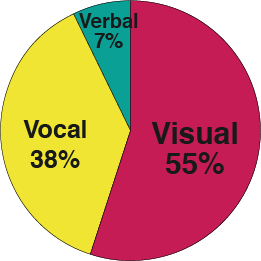
\includegraphics[width=50mm,bb=0 0 261 261]{mehrabian.jpg}}
    \end{center}
    \caption{メラビアンの法則}
    \label{fig:mehrabian}
\end{figure}


\subsection{人との繋がり形成の多様化}
人との繋がりについて書く

\section{本文書の構成}

第1章の最後は、文書全体の構成を大まかに書くとよいらしい。

第\ref{chap:introduction}章では本テンプレートの概要みたいなものを書いた。第\ref{chap:howto}章では、本テンプレートの使い方を説明する。第\ref{chap:latex}章で図表や数式の挿入など代表的な\LaTeX コマンドを解説する。第\ref{chap:conclusion}章では、『序論』で始めたら『結論』で終われと書いた手前書かざるを得ないので、なにか結論らしいことを書く。付録として、テンプレートのサンプルになるように無理矢理ゴミを添付する。
  % 序論
%\chapter{本テンプレートの使い方}
\label{chap:howto}

本章では、本テンプレートの具体的な使用方法を解説する。基本的には、{\tt main.tex} を上から順に修正していけばよいだけ。


\section{テンプレートの構成}

このテンプレートは、表\ref{tb:files}のファイルで構成されている。

\begin{table}[htbp]
  \caption{構成ファイル}
  \label{tb:files}
  \begin{center}\begin{tabular}{c|l}
    \hline
    ファイル名&用途\\\hline\hline
    {\tt main.tex}&メインのファイル。これを編集していく\\\hline
    {\tt thesis.sty}&論文のスタイルを定義したファイル。基本的には手は加えない\\\hline
    {\tt *.tex}&{\tt main.tex}に{\tt include}されるファイル群\\\hline
    {\tt *.eps}&画像ファイル\\\hline
    {\tt main.bib}&参考文献用のBibTeXファイル\\\hline
    {\tt Makefile}&Makefile。次節以降で説明\\\hline
    {\tt .gitignore}&Git用設定ファイル\\\hline
  \end{tabular}\end{center}
\end{table}

\section{コンパイル}
このテンプレートの\LaTeX ファイルをコンパイルしてPDFファイルを生成するには、ターミナルを開いて以下のようにする。

\begin{itembox}[l]{コマンド実行例}
\begin{verbatim}
% make
\end{verbatim}
\end{itembox}

こうすることで、\verb|platex|コマンド、\verb|pbibtex|コマンド、\verb|platex|コマンド2回、\verb|dvipdfmx|コマンドが全て実行され、{\tt main.pdf}が生成される。

コンパイルによって生成されたファイルを全て消すには、以下のようにする。

\begin{itembox}[l]{コマンド実行例}
\begin{verbatim}
% make clean
\end{verbatim}
\end{itembox}

\section{設定}

以下、{\tt main.tex}に対して行うべき設定を、このファイルの中に書いてある順に沿って説明する。

\subsection{論文全体の言語の設定}
\label{sec:lang}

\begin{itembox}[l]{{\tt main.tex}}
\begin{verbatim}
\japanesetrue	% 論文全体を日本語で書く(英語で書くならコメントアウト)
\end{verbatim}
\end{itembox}

ここでは論文全体の言語を設定する。日本語に設定すれば、『章』『目次』『謝辞』などが日本語で出力されて、行頭のインデントなども日本語の仕様になる。英語にした場合は、これらはそれぞれ『Chapter』『Table of Contents』『Acknowledgment』な体裁になる。インデントも行間も、英語用の設定が適用される。

\verb|\japanesetrue| をコメントアウトしなければ日本語に、コメントアウトすれば英語に設定される。


\subsection{余白の設定}

\begin{itembox}[l]{{\tt main.tex}}
\begin{verbatim}
\bindermode	% バインダ用余白設定
\end{verbatim}
\end{itembox}

このテンプレートの出力はA4用紙。ここではこれの四辺の余白を設定する。

最終的にバインダーで綴じて提出する場合、余白を左右対称にしてしまうと、見かけ上のバランスがとても悪くなる。これを解消するため、あらかじめ左側の余白を大きく取っておく。

\verb|\bindermode| をコメントアウトしなければ左綴じ用の余白に、コメントアウトすれば左右対称の余白に設定される。

両面印刷の場合、偶数ページと奇数ページで余白を広くとるべき側が違うので、\verb|documentclass| でこれを設定する。

\begin{itembox}[l]{{\tt main.tex}}
\begin{verbatim}
% 両面印刷の場合。余白を綴じ側に作って右起こし。
\documentclass[a4j,twoside,openright,11pt]{jreport}
% 片面印刷の場合。
%\documentclass[a4j,11pt]{jreport}
\end{verbatim}
\end{itembox}

両面印刷の場合は \verb|twoside| を使用する。\verb|openright| を使うと章のはじまりが必ず右側のページに来るようになる。

\subsection{論文情報の設定}
\label{sec:meta}

\begin{itembox}[l]{{\tt main.tex}}
\begin{verbatim}
% 日本語情報(必要なら)
\jclass  {修士論文}                             % 論文種別
\jtitle    {修士論文用 \LaTeX\ テンプレート}    % タイトル。改行する場合は\\を入れる
\juniv    {慶應義塾大学大学院}                  % 大学名
\jfaculty  {政策・メディア研究科}               % 学部、学科
\jauthor  {ほげ山 ふう助}                       % 著者
\jhyear  {24}                                   % 平成○年度
\jsyear  {2012}                                 % 西暦○年度
\jkeyword  {\LaTeX、テンプレート、修士論文}     % 論文のキーワード
\jproject{インタラクションデザインプロジェクト} %プロジェクト名
\jdate{2013年1月}

% 英語情報(必要なら)
\eclass  {Master's Thesis}                            % 論文種別
\etitle    {A \LaTeX Template for Master Thesis}      % タイトル。改行する場合は\\を入れる
\euniv  {Keio University}                             % 大学名
\efaculty  {Graduate School of Media and Governance}  % 学部、学科
\eauthor  {Fusuke Hogeyama}                           % 著者
\eyear  {2012}                                        % 西暦○年度
\ekeyword  {\LaTeX, Templete, Master Thesis}          % 論文のキーワード
\eproject{Interaction Design Project}                 %プロジェクト名
\edate{January 2013}
\end{verbatim}
\end{itembox}

ここでは論文のタイトルや著者の氏名などのメタデータを記述する。ここで書いたデータは、表紙とアブストラクトのページに使われる。必ずしも日本語と英語の両方を設定しなければいけないわけではなくて、自分が必要とする方だけ記述すればよい。

タイトルが長過ぎる場合は、表紙やアブストラクトのページでは自動で折り返して出力される。もし改行位置を自分で指定したい場合は、その場所に \verb|\\| を入力する。


\section{出力}

\verb|\begin{document}| から \verb|\end{document}| に記述した部分が、実際に{\tt DVI}(最終的には{\tt PDF})ファイルとして出力される。

\subsection{外部ファイルの読み込み({\tt include})}

出力部分の具体的な説明の前に、外部ファイルを読み込む方法を説明する。

\verb|\begin{document}| から \verb|\end{document}| の間では、\verb|\include| コマンドを使うことで、別の {\tt *.tex} ファイルを読み込ませられる。

\begin{itembox}[l]{{\tt include}しない場合}
\begin{itembox}[l]{{\tt main.tex}}
\begin{verbatim}
\begin{document}
  \begin{jabstract}
  ほげほげ
  \end{jabstract}
\end{document}
\end{verbatim}
\end{itembox}
\end{itembox}

\begin{itembox}[l]{{\tt include}する場合}
\begin{minipage}{0.5\hsize}
\begin{itembox}[l]{{\tt main.tex}}
\begin{verbatim}
\begin{document}
\chapter{序論}
\label{chap:introduction}

本章では, はじめに本研究における背景を述べる.ついで, 問題意識を踏まえた上での目的, 製作者の仮説を述べる. 最後に本論文の構成を示す.

\section{背景}
本節では, 本研究の背景としと人と人との繋がりで構成されている現代社会について述べる. ついで人との繋がり形成におけるコミュニケーション上での表情の重要性を述べ, 最後に現代社会における人との関係性を構築する手段が多様化している様子を述べる.

%\begin{quotation}
%\end{quotation} 引用をする際にはこれを使用する

\subsection{人と人との繋がりで構成されている社会}
ヒトは誕生から現代にかけて社会を形成し,その中で集団を作って生活を送ってきた. 社会性をもつ生き物として, 交友関係を広げ, 協力をして日々を生きている. 職場, 学校, 近所, そして家族など人との繋がりは必要不可欠な要素である. 日本人の平均寿命はWHOの調査で84.2歳\cite{WHO_reserch}と言われ,1日1人と出会ったとしても30733人と出会うことになり, 人と関わることなしに生活することは不可能である.
\subsection{コミュニケーションにおける表情の重要性}
人との関係構築をする際にはコミュニケーションが必要不可欠である. コミュニケーションにおいて非言語コミュニケーションがもっとも重要とAlbert Mehrabian\cite{rule_of_Mehrabian}は述べており, 会話中の相手の受け取る情報量は非言語コミュニケーションが93\% を占め, その中でも視覚情報は55\% を占めると言われている. その中でも,人の表情はその人の内面を表しており相手のことを判断するときに重要な判断材料となる.
%表情,笑顔が重要な理由を出す
\begin{figure}[htbp]
    \begin{center}
       \fbox{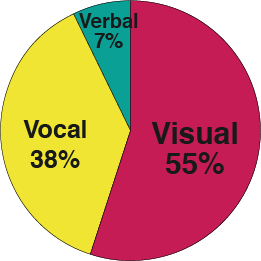
\includegraphics[width=50mm,bb=0 0 261 261]{mehrabian.jpg}}
    \end{center}
    \caption{メラビアンの法則}
    \label{fig:mehrabian}
\end{figure}


\subsection{人との繋がり形成の多様化}
人との繋がりについて書く

\section{本文書の構成}

第1章の最後は、文書全体の構成を大まかに書くとよいらしい。

第\ref{chap:introduction}章では本テンプレートの概要みたいなものを書いた。第\ref{chap:howto}章では、本テンプレートの使い方を説明する。第\ref{chap:latex}章で図表や数式の挿入など代表的な\LaTeX コマンドを解説する。第\ref{chap:conclusion}章では、『序論』で始めたら『結論』で終われと書いた手前書かざるを得ないので、なにか結論らしいことを書く。付録として、テンプレートのサンプルになるように無理矢理ゴミを添付する。
 % 01.texをinclude
\end{document}
\end{verbatim}
\end{itembox}
\end{minipage}
\begin{minipage}{0.5\hsize}
\begin{itembox}[l]{{\tt 01.tex}}
\begin{verbatim}
\begin{jabstract}
ほげほげ
\end{jabstract}
\end{verbatim}
\end{itembox}
\end{minipage}
\end{itembox}

{\tt include}しない場合とする場合を比較するとこのとおり。どちらも出力結果は一緒。{\tt include}する場合は、読み込ませたい箇所に、読み込ませたい{\tt *.tex}ファイルの名前を、拡張子を除いて \verb|\include| コマンドで書けばよい。

\verb|\include| コマンドを用いるか用いないかは、たぶん文書量や個人の好みに依る。例えば章ごとに別のファイルにしておけば、修正箇所を探すときの手間が多少は省けるかもしれない。Gitで人と共有しつつ校正を頼むときにもファイルが分かれていたほうがコンフリクトを起こしにくい。


\subsection{表紙の出力}

\begin{itembox}[l]{{\tt main.tex}}
\begin{verbatim}
\ifjapanese
  \jmaketitle    % 表紙(日本語)
\else
  \emaketitle    % 表紙(英語)
\fi
\end{verbatim}
\end{itembox}

最初に、表紙を出力する。

\verb|\jmaketitle| が実行されると日本語の表紙が、\verb|\emaketitle| が実行されると英語の表紙がそれぞれ出力される。日本語の表紙には、第\ref{sec:meta}節で設定したうちの日本語の情報が、英語の表紙には同節で設定したうち英語の情報が、それぞれ参照されて、表記される。

デフォルトでは第\ref{sec:lang}説で設定した言語の表紙のみが出力されるようになっている。

\subsection{アブストラクトの出力}

\begin{itembox}[l]{{\tt main.tex}}
\begin{verbatim}
% ■ アブストラクトの出力 ■
%	◆書式:
%		begin{jabstract}〜end{jabstract}	:日本語のアブストラクト
%		begin{eabstract}〜end{eabstract}	:英語のアブストラクト
%		※ 不要ならばコマンドごと消せば出力されない。



% 日本語のアブストラクト
\begin{jabstract}
人が暮らす社会は人と人との繋がりで構成されている.人間関係を構築する際には
コミュニケーションが必要であり, その中でも表情などの非言語コミュニケーション,
特に笑顔は大きく影響を及ぼす.
人との繋がり形成の場が多様化し,入り口が広くなった分情報量が多くなり,整理がうまく行えていない現状がある.若者がテキストベースのやりとりを行った後, 実際に会った際には相手にがっかりするケースが非常に多くなっている.
本研究の目的は笑顔の作り方からお互いを分析し, 人と人との繋がりを助長するシステムの構築をである.
自身の笑い方と, 魅力を感じる笑い方にはどのような関係性があるのかを考察し, 嗜好傾向を分析する.
データに基づく分析を行うことで, より最適な相手をユーザーに表示し, よりよい出会いの機会提供を助長することを目指す.
%<位置変更>
本研究ではユーザーの中立の表情から,笑顔になる過程を画像処理し,数値化するシステムを作成する.
表情の特徴点を示した動画に対してユーザーに順位づけをさせ, ユーザー自身の笑顔の作り方と表情ベースにおけるユーザーごと,全ユーザーに共通した嗜好傾向の分析を行った.

慶應義塾大学湘南藤沢キャンパス主催のOpen Reserch Forumにてデモンストレーションおよび評価実験を行い, 41人の来場者のデータを取得した. 破損データを除く36個の笑顔動画データからCambridge大学が開発したOpenFaceに含まれる,Facial Action Units(FAU)の値を算出しユーザーごとに嗜好傾向分析を行った.
分析の結果, 人は一度顔の筋肉を弛緩してから笑顔になるユーザーに嗜好傾向があることが判明した.

%<変更>
今後の展望として, 本システムはより多くのデータを収集, ユーザーの内面状態を組み込むことで
仕事または結婚時のパートナー選択に有益な情報を提供することが可能である.
情報過多になっている現代社会において, ユーザーにとって適切なデータ提供を行い,
より良い人間関係の構築をする機会を提供することが可能になると考えられる.
本研究が, 人と人との良縁を結ぶ役割を担うようなシステムになることを期待する.

\end{jabstract}

% 英語のアブストラクト
\begin{eabstract}


  The society we live in is constructed from the connections between the people.
  In order to establish this relationship, communication is crucial, especially non-verbal communication,
  and factors such as smiling can have significant influences.
  The way in which people connect have become diverse, and with this, more information is available;
  however this information has still yet to be organized.
  In the younger generations,
  many may often be disappointed when actually meeting the people that they had previously “met” online via text.
  The purpose of this research is to build a system that promotes the connection between people based on analyzing each other based on their smiles.
  This system finds a correlation between one’s smile and the smile that they prefer, and analyzes the inclination.
  By performing data-based analysis, I aim to make connect the most optimal partners to users, and encourage better encounters.

  In this research we create a system that digitizes the process in which the users smile from a neutral expression, via image processing.
  Based on the calculated values,
  the system displays videos from the database of the process in which people smile.
  These videos show the featured points in place of the person’s face.
  The users then rank the videos, after which the analysis is conducted on each user,
  and the users as a group, on how the users smile, and on their smile preferences.

  I conducted demonstrations and evaluation experiments at the Open Research Forum hosted by Keio University Shonan Fujisawa Campus,
  and obtained datasets from 41 visitors.
  I got the value of Facial Action Units (FAU) included in OpenFace developed by Cambridge University from 36 smile video data excluding damaged data,
  and analyzed the inclination tendency for each users.
  As a result of the analysis, it was found that people tend to prefer people who relax their facial muscles before smiling.

In the future,
it will be possible to provide beneficial information on partner selection at work or marriage,
when the system will collect more data and consider users' insides.
In today's information overload society, this system provides users with appropriate data,
It will be possible to provide an opportunity to build better human relationships.
I expect that this system will play a critical role in connecting people.

\end{eabstract}

\begin{comment}
<修正前>
本研究ではユーザーの中立の表情から,笑顔になる過程を画像処理し,数値化するシステムを作成する.
算出した値を元にデータベースにある笑顔動画データをユーザーに人物が特定できないように, 表情の特徴68点の動きのみを5人分表示する.
選ばれた特徴点を示した動画に対してユーザーに順位づけをさせ, ユーザー自身の笑顔の作り方と表情ベースにおけるユーザーごと,
全ユーザーに共通した嗜好傾向の分析を行った.
人が暮らす社会は人と人との繋がりで構成されている.人間関係を構築する際には
コミュニケーションが必要であり, その中でも表情などの非言語コミュニケーション,
特に笑顔は大きく影響を及ぼす.
人との繋がり形成の場が多様化し,入り口が広くなった分情報量が多くなり,整理がうまく行えていない現状がある.若者がテキストベースのやりとりを行った後, 実際に会った際には相手にがっかりするケースが非常に多くなっている.
本研究の目的は笑顔の作り方からお互いを分析し, 人と人との繋がりを助長するシステムの構築をである.
自身の笑い方と, 魅力を感じる笑い方にはどのような関係性があるのかを考察し, 嗜好傾向を分析する.
データに基づく分析を行うことで, より最適な相手をユーザーに表示し, よりよい出会いの機会提供を助長することを目指す.
慶應義塾大学湘南藤沢キャンパス主催のOpen Reserch Forumにてデモンストレーションおよび評価実験を行い, 41人の来場者のデータを取得した. 破損データを除く36個の笑顔動画データからCambridge大学が開発したOpenFaceに含まれる,Facial Action Units(FAU)の値を算出しユーザーごとに嗜好傾向分析を行った.
分析の結果, 人は一度顔の筋肉を弛緩してから笑顔になるユーザーに嗜好傾向があることが判明した.
今後の展望として, 中澤研究室が関与する健康情報コンソーシアムのTeamSmileで作成したSmileMeterに本システムのモジュールを組み込むことでより幅広く多くのデータの取得を可能にし,
人と人を繋ぐ役割を担うようなシステムになることを期待する.
\end{comment}

\begin{comment}
In this research we create a system that digitizes the process in which the users smile from a neutral expression, via image processing.
Based on the calculated values,
the system displays five videos from the database of the process in which people smile.
These five videos show the 68 featured points in place of the person’s face
so that the users’ cannot identify the person from the video.
The users then rank the videos, after which the analysis is conducted on each user,
and the users as a group, on how the users smile, and on their smile preferences.
The society we live in is constructed from the connections between the people.
In order to establish this relationship, communication is crucial, especially non-verbal communication,
and factors such as smiling can have significant influences.
The way in which people connect have become diverse, and with this, more information is available;
however this information has still yet to be organized.
In the younger generations,
many may often be disappointed when actually meeting the people that they had previously “met” online via text.
The purpose of this research is to build a system that promotes the connection between people based on analyzing each other based on their smiles.
This system finds a correlation between one’s smile and the smile that they prefer, and analyzes the inclination.
By performing data-based analysis, I aim to make connect the most optimal partners to users, and encourage better encounters.
I conducted demonstrations and evaluation experiments at the Open Research Forum hosted by Keio University Shonan Fujisawa Campus,
and obtained datasets from 41 visitors.
I got the value of Facial Action Units (FAU) included in OpenFace developed by Cambridge University from 36 smile video data excluding damaged data,
and analyzed the inclination tendency for each users.
As a result of the analysis, it was found that people tend to prefer people who relax their facial muscles before smiling.
In the future, TeamSmile in health information consortium related with Nakazawa Laboratory,
will incorporate the module of this system into the SmileMeter to enable the acquisition of more and more data.
I expect that this system will play a critical role in connecting people.

\end{comment}
	% アブストラクト。要独自コマンド、include先参照のこと
\end{verbatim}
\end{itembox}

表紙の次は、アブストラクト。

アブストラクトを出力するには、出力したい位置に、指定のコマンドを用いて文章を書き下せばよい。{\tt main.tex}に直接書いてもよいし、先述した \verb|\include| コマンドを利用して{\tt include}してもよい。

\verb|\begin{jabstract}| から \verb|\end{jabstract}| の間に書いた文章が日本語のアブストラクトとして、\verb|\begin{eabstract}| から \verb|\end{eabstract}| の間に書いた文章が英語のアブストラクトとして、それぞれ独立したページに出力される。

アブストラクトのページには、論文のタイトルやキーワードなどが、第\ref{sec:meta}節で設定した情報をもとにして自動で表記される。

日本語か英語のどちらか一方のみでよい場合は、不要な言語の方のコマンドを削除すればよい。これは、\verb|\begin| と \verb|\end| というコマンド自身も含めて削除する、ということで、\verb|\begin| と \verb|\end| の間を空っぽにするという意味ではないので注意。



\subsection{目次類の出力}
\label{sec:toc}

\begin{itembox}[l]{{\tt main.tex}}
\begin{verbatim}
\tableofcontents	% 目次
\listoffigures		% 表目次
\listoftables		% 図目次
\end{verbatim}
\end{itembox}

アブストラクトの次に、目次。文書の目次、図の目次、表の目次の三種類。

目次類を出力するには、出力したい位置に指定のコマンドを書けばよい。

これらのコマンドは、コンパイル時点での一時ファイル\footnote{{\tt *.toc}、{\tt *.lof}、{\tt *.lot}}の情報を、目次として体裁を整えて出力するもの。一時ファイルは、\verb|\begin{document}| から \verb|\end{document}| の間の章や節、図や表をコンパイルするときに、ついでに情報を取得しておいて生成される。

つまり気をつけなければいけないのは、コンパイルを一回しただけでは、一時ファイルが最新の状態に更新されるだけで、肝心の目次は正しい情報では出力されないということ。目次類を正しい情報で出力するには、最低二回のコンパイルが必要。一回目のコンパイルで一時ファイルが最新の情報に更新されて、二回目のコンパイルで初めて、その最新の一時ファイルの情報をもとに目次が出力される。

だから、文書に何らかの修正をして保存したあとは、最低でも二回、連続してコンパイルしないといけないことに注意する。

図や表を一つも使用していない場合は、目次名のみが書かれた空白のページが出力される。もしこれが不要な場合は、該当するコマンドをコメントアウトすればよい。


\subsection{本文の出力}

\begin{itembox}[l]{{\tt main.tex}}
\begin{verbatim}
\chapter{序論}
\label{chap:introduction}

本章では, はじめに本研究における背景を述べる.ついで, 問題意識を踏まえた上での目的, 製作者の仮説を述べる. 最後に本論文の構成を示す.

\section{背景}
本節では, 本研究の背景としと人と人との繋がりで構成されている現代社会について述べる. ついで人との繋がり形成におけるコミュニケーション上での表情の重要性を述べ, 最後に現代社会における人との関係性を構築する手段が多様化している様子を述べる.

%\begin{quotation}
%\end{quotation} 引用をする際にはこれを使用する

\subsection{人と人との繋がりで構成されている社会}
ヒトは誕生から現代にかけて社会を形成し,その中で集団を作って生活を送ってきた. 社会性をもつ生き物として, 交友関係を広げ, 協力をして日々を生きている. 職場, 学校, 近所, そして家族など人との繋がりは必要不可欠な要素である. 日本人の平均寿命はWHOの調査で84.2歳\cite{WHO_reserch}と言われ,1日1人と出会ったとしても30733人と出会うことになり, 人と関わることなしに生活することは不可能である.
\subsection{コミュニケーションにおける表情の重要性}
人との関係構築をする際にはコミュニケーションが必要不可欠である. コミュニケーションにおいて非言語コミュニケーションがもっとも重要とAlbert Mehrabian\cite{rule_of_Mehrabian}は述べており, 会話中の相手の受け取る情報量は非言語コミュニケーションが93\% を占め, その中でも視覚情報は55\% を占めると言われている. その中でも,人の表情はその人の内面を表しており相手のことを判断するときに重要な判断材料となる.
%表情,笑顔が重要な理由を出す
\begin{figure}[htbp]
    \begin{center}
       \fbox{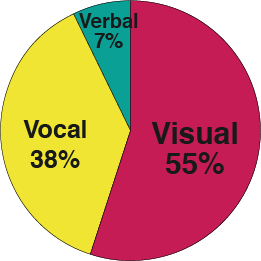
\includegraphics[width=50mm,bb=0 0 261 261]{mehrabian.jpg}}
    \end{center}
    \caption{メラビアンの法則}
    \label{fig:mehrabian}
\end{figure}


\subsection{人との繋がり形成の多様化}
人との繋がりについて書く

\section{本文書の構成}

第1章の最後は、文書全体の構成を大まかに書くとよいらしい。

第\ref{chap:introduction}章では本テンプレートの概要みたいなものを書いた。第\ref{chap:howto}章では、本テンプレートの使い方を説明する。第\ref{chap:latex}章で図表や数式の挿入など代表的な\LaTeX コマンドを解説する。第\ref{chap:conclusion}章では、『序論』で始めたら『結論』で終われと書いた手前書かざるを得ないので、なにか結論らしいことを書く。付録として、テンプレートのサンプルになるように無理矢理ゴミを添付する。
	% 本文1
\chapter{本テンプレートの使い方}
\label{chap:howto}

本章では、本テンプレートの具体的な使用方法を解説する。基本的には、{\tt main.tex} を上から順に修正していけばよいだけ。


\section{テンプレートの構成}

このテンプレートは、表\ref{tb:files}のファイルで構成されている。

\begin{table}[htbp]
  \caption{構成ファイル}
  \label{tb:files}
  \begin{center}\begin{tabular}{c|l}
    \hline
    ファイル名&用途\\\hline\hline
    {\tt main.tex}&メインのファイル。これを編集していく\\\hline
    {\tt thesis.sty}&論文のスタイルを定義したファイル。基本的には手は加えない\\\hline
    {\tt *.tex}&{\tt main.tex}に{\tt include}されるファイル群\\\hline
    {\tt *.eps}&画像ファイル\\\hline
    {\tt main.bib}&参考文献用のBibTeXファイル\\\hline
    {\tt Makefile}&Makefile。次節以降で説明\\\hline
    {\tt .gitignore}&Git用設定ファイル\\\hline
  \end{tabular}\end{center}
\end{table}

\section{コンパイル}
このテンプレートの\LaTeX ファイルをコンパイルしてPDFファイルを生成するには、ターミナルを開いて以下のようにする。

\begin{itembox}[l]{コマンド実行例}
\begin{verbatim}
% make
\end{verbatim}
\end{itembox}

こうすることで、\verb|platex|コマンド、\verb|pbibtex|コマンド、\verb|platex|コマンド2回、\verb|dvipdfmx|コマンドが全て実行され、{\tt main.pdf}が生成される。

コンパイルによって生成されたファイルを全て消すには、以下のようにする。

\begin{itembox}[l]{コマンド実行例}
\begin{verbatim}
% make clean
\end{verbatim}
\end{itembox}

\section{設定}

以下、{\tt main.tex}に対して行うべき設定を、このファイルの中に書いてある順に沿って説明する。

\subsection{論文全体の言語の設定}
\label{sec:lang}

\begin{itembox}[l]{{\tt main.tex}}
\begin{verbatim}
\japanesetrue	% 論文全体を日本語で書く(英語で書くならコメントアウト)
\end{verbatim}
\end{itembox}

ここでは論文全体の言語を設定する。日本語に設定すれば、『章』『目次』『謝辞』などが日本語で出力されて、行頭のインデントなども日本語の仕様になる。英語にした場合は、これらはそれぞれ『Chapter』『Table of Contents』『Acknowledgment』な体裁になる。インデントも行間も、英語用の設定が適用される。

\verb|\japanesetrue| をコメントアウトしなければ日本語に、コメントアウトすれば英語に設定される。


\subsection{余白の設定}

\begin{itembox}[l]{{\tt main.tex}}
\begin{verbatim}
\bindermode	% バインダ用余白設定
\end{verbatim}
\end{itembox}

このテンプレートの出力はA4用紙。ここではこれの四辺の余白を設定する。

最終的にバインダーで綴じて提出する場合、余白を左右対称にしてしまうと、見かけ上のバランスがとても悪くなる。これを解消するため、あらかじめ左側の余白を大きく取っておく。

\verb|\bindermode| をコメントアウトしなければ左綴じ用の余白に、コメントアウトすれば左右対称の余白に設定される。

両面印刷の場合、偶数ページと奇数ページで余白を広くとるべき側が違うので、\verb|documentclass| でこれを設定する。

\begin{itembox}[l]{{\tt main.tex}}
\begin{verbatim}
% 両面印刷の場合。余白を綴じ側に作って右起こし。
\documentclass[a4j,twoside,openright,11pt]{jreport}
% 片面印刷の場合。
%\documentclass[a4j,11pt]{jreport}
\end{verbatim}
\end{itembox}

両面印刷の場合は \verb|twoside| を使用する。\verb|openright| を使うと章のはじまりが必ず右側のページに来るようになる。

\subsection{論文情報の設定}
\label{sec:meta}

\begin{itembox}[l]{{\tt main.tex}}
\begin{verbatim}
% 日本語情報(必要なら)
\jclass  {修士論文}                             % 論文種別
\jtitle    {修士論文用 \LaTeX\ テンプレート}    % タイトル。改行する場合は\\を入れる
\juniv    {慶應義塾大学大学院}                  % 大学名
\jfaculty  {政策・メディア研究科}               % 学部、学科
\jauthor  {ほげ山 ふう助}                       % 著者
\jhyear  {24}                                   % 平成○年度
\jsyear  {2012}                                 % 西暦○年度
\jkeyword  {\LaTeX、テンプレート、修士論文}     % 論文のキーワード
\jproject{インタラクションデザインプロジェクト} %プロジェクト名
\jdate{2013年1月}

% 英語情報(必要なら)
\eclass  {Master's Thesis}                            % 論文種別
\etitle    {A \LaTeX Template for Master Thesis}      % タイトル。改行する場合は\\を入れる
\euniv  {Keio University}                             % 大学名
\efaculty  {Graduate School of Media and Governance}  % 学部、学科
\eauthor  {Fusuke Hogeyama}                           % 著者
\eyear  {2012}                                        % 西暦○年度
\ekeyword  {\LaTeX, Templete, Master Thesis}          % 論文のキーワード
\eproject{Interaction Design Project}                 %プロジェクト名
\edate{January 2013}
\end{verbatim}
\end{itembox}

ここでは論文のタイトルや著者の氏名などのメタデータを記述する。ここで書いたデータは、表紙とアブストラクトのページに使われる。必ずしも日本語と英語の両方を設定しなければいけないわけではなくて、自分が必要とする方だけ記述すればよい。

タイトルが長過ぎる場合は、表紙やアブストラクトのページでは自動で折り返して出力される。もし改行位置を自分で指定したい場合は、その場所に \verb|\\| を入力する。


\section{出力}

\verb|\begin{document}| から \verb|\end{document}| に記述した部分が、実際に{\tt DVI}(最終的には{\tt PDF})ファイルとして出力される。

\subsection{外部ファイルの読み込み({\tt include})}

出力部分の具体的な説明の前に、外部ファイルを読み込む方法を説明する。

\verb|\begin{document}| から \verb|\end{document}| の間では、\verb|\include| コマンドを使うことで、別の {\tt *.tex} ファイルを読み込ませられる。

\begin{itembox}[l]{{\tt include}しない場合}
\begin{itembox}[l]{{\tt main.tex}}
\begin{verbatim}
\begin{document}
  \begin{jabstract}
  ほげほげ
  \end{jabstract}
\end{document}
\end{verbatim}
\end{itembox}
\end{itembox}

\begin{itembox}[l]{{\tt include}する場合}
\begin{minipage}{0.5\hsize}
\begin{itembox}[l]{{\tt main.tex}}
\begin{verbatim}
\begin{document}
\chapter{序論}
\label{chap:introduction}

本章では, はじめに本研究における背景を述べる.ついで, 問題意識を踏まえた上での目的, 製作者の仮説を述べる. 最後に本論文の構成を示す.

\section{背景}
本節では, 本研究の背景としと人と人との繋がりで構成されている現代社会について述べる. ついで人との繋がり形成におけるコミュニケーション上での表情の重要性を述べ, 最後に現代社会における人との関係性を構築する手段が多様化している様子を述べる.

%\begin{quotation}
%\end{quotation} 引用をする際にはこれを使用する

\subsection{人と人との繋がりで構成されている社会}
ヒトは誕生から現代にかけて社会を形成し,その中で集団を作って生活を送ってきた. 社会性をもつ生き物として, 交友関係を広げ, 協力をして日々を生きている. 職場, 学校, 近所, そして家族など人との繋がりは必要不可欠な要素である. 日本人の平均寿命はWHOの調査で84.2歳\cite{WHO_reserch}と言われ,1日1人と出会ったとしても30733人と出会うことになり, 人と関わることなしに生活することは不可能である.
\subsection{コミュニケーションにおける表情の重要性}
人との関係構築をする際にはコミュニケーションが必要不可欠である. コミュニケーションにおいて非言語コミュニケーションがもっとも重要とAlbert Mehrabian\cite{rule_of_Mehrabian}は述べており, 会話中の相手の受け取る情報量は非言語コミュニケーションが93\% を占め, その中でも視覚情報は55\% を占めると言われている. その中でも,人の表情はその人の内面を表しており相手のことを判断するときに重要な判断材料となる.
%表情,笑顔が重要な理由を出す
\begin{figure}[htbp]
    \begin{center}
       \fbox{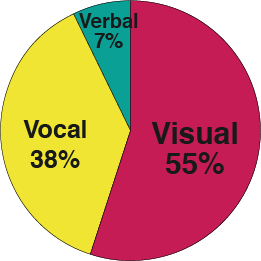
\includegraphics[width=50mm,bb=0 0 261 261]{mehrabian.jpg}}
    \end{center}
    \caption{メラビアンの法則}
    \label{fig:mehrabian}
\end{figure}


\subsection{人との繋がり形成の多様化}
人との繋がりについて書く

\section{本文書の構成}

第1章の最後は、文書全体の構成を大まかに書くとよいらしい。

第\ref{chap:introduction}章では本テンプレートの概要みたいなものを書いた。第\ref{chap:howto}章では、本テンプレートの使い方を説明する。第\ref{chap:latex}章で図表や数式の挿入など代表的な\LaTeX コマンドを解説する。第\ref{chap:conclusion}章では、『序論』で始めたら『結論』で終われと書いた手前書かざるを得ないので、なにか結論らしいことを書く。付録として、テンプレートのサンプルになるように無理矢理ゴミを添付する。
 % 01.texをinclude
\end{document}
\end{verbatim}
\end{itembox}
\end{minipage}
\begin{minipage}{0.5\hsize}
\begin{itembox}[l]{{\tt 01.tex}}
\begin{verbatim}
\begin{jabstract}
ほげほげ
\end{jabstract}
\end{verbatim}
\end{itembox}
\end{minipage}
\end{itembox}

{\tt include}しない場合とする場合を比較するとこのとおり。どちらも出力結果は一緒。{\tt include}する場合は、読み込ませたい箇所に、読み込ませたい{\tt *.tex}ファイルの名前を、拡張子を除いて \verb|\include| コマンドで書けばよい。

\verb|\include| コマンドを用いるか用いないかは、たぶん文書量や個人の好みに依る。例えば章ごとに別のファイルにしておけば、修正箇所を探すときの手間が多少は省けるかもしれない。Gitで人と共有しつつ校正を頼むときにもファイルが分かれていたほうがコンフリクトを起こしにくい。


\subsection{表紙の出力}

\begin{itembox}[l]{{\tt main.tex}}
\begin{verbatim}
\ifjapanese
  \jmaketitle    % 表紙(日本語)
\else
  \emaketitle    % 表紙(英語)
\fi
\end{verbatim}
\end{itembox}

最初に、表紙を出力する。

\verb|\jmaketitle| が実行されると日本語の表紙が、\verb|\emaketitle| が実行されると英語の表紙がそれぞれ出力される。日本語の表紙には、第\ref{sec:meta}節で設定したうちの日本語の情報が、英語の表紙には同節で設定したうち英語の情報が、それぞれ参照されて、表記される。

デフォルトでは第\ref{sec:lang}説で設定した言語の表紙のみが出力されるようになっている。

\subsection{アブストラクトの出力}

\begin{itembox}[l]{{\tt main.tex}}
\begin{verbatim}
% ■ アブストラクトの出力 ■
%	◆書式:
%		begin{jabstract}〜end{jabstract}	:日本語のアブストラクト
%		begin{eabstract}〜end{eabstract}	:英語のアブストラクト
%		※ 不要ならばコマンドごと消せば出力されない。



% 日本語のアブストラクト
\begin{jabstract}
人が暮らす社会は人と人との繋がりで構成されている.人間関係を構築する際には
コミュニケーションが必要であり, その中でも表情などの非言語コミュニケーション,
特に笑顔は大きく影響を及ぼす.
人との繋がり形成の場が多様化し,入り口が広くなった分情報量が多くなり,整理がうまく行えていない現状がある.若者がテキストベースのやりとりを行った後, 実際に会った際には相手にがっかりするケースが非常に多くなっている.
本研究の目的は笑顔の作り方からお互いを分析し, 人と人との繋がりを助長するシステムの構築をである.
自身の笑い方と, 魅力を感じる笑い方にはどのような関係性があるのかを考察し, 嗜好傾向を分析する.
データに基づく分析を行うことで, より最適な相手をユーザーに表示し, よりよい出会いの機会提供を助長することを目指す.
%<位置変更>
本研究ではユーザーの中立の表情から,笑顔になる過程を画像処理し,数値化するシステムを作成する.
表情の特徴点を示した動画に対してユーザーに順位づけをさせ, ユーザー自身の笑顔の作り方と表情ベースにおけるユーザーごと,全ユーザーに共通した嗜好傾向の分析を行った.

慶應義塾大学湘南藤沢キャンパス主催のOpen Reserch Forumにてデモンストレーションおよび評価実験を行い, 41人の来場者のデータを取得した. 破損データを除く36個の笑顔動画データからCambridge大学が開発したOpenFaceに含まれる,Facial Action Units(FAU)の値を算出しユーザーごとに嗜好傾向分析を行った.
分析の結果, 人は一度顔の筋肉を弛緩してから笑顔になるユーザーに嗜好傾向があることが判明した.

%<変更>
今後の展望として, 本システムはより多くのデータを収集, ユーザーの内面状態を組み込むことで
仕事または結婚時のパートナー選択に有益な情報を提供することが可能である.
情報過多になっている現代社会において, ユーザーにとって適切なデータ提供を行い,
より良い人間関係の構築をする機会を提供することが可能になると考えられる.
本研究が, 人と人との良縁を結ぶ役割を担うようなシステムになることを期待する.

\end{jabstract}

% 英語のアブストラクト
\begin{eabstract}


  The society we live in is constructed from the connections between the people.
  In order to establish this relationship, communication is crucial, especially non-verbal communication,
  and factors such as smiling can have significant influences.
  The way in which people connect have become diverse, and with this, more information is available;
  however this information has still yet to be organized.
  In the younger generations,
  many may often be disappointed when actually meeting the people that they had previously “met” online via text.
  The purpose of this research is to build a system that promotes the connection between people based on analyzing each other based on their smiles.
  This system finds a correlation between one’s smile and the smile that they prefer, and analyzes the inclination.
  By performing data-based analysis, I aim to make connect the most optimal partners to users, and encourage better encounters.

  In this research we create a system that digitizes the process in which the users smile from a neutral expression, via image processing.
  Based on the calculated values,
  the system displays videos from the database of the process in which people smile.
  These videos show the featured points in place of the person’s face.
  The users then rank the videos, after which the analysis is conducted on each user,
  and the users as a group, on how the users smile, and on their smile preferences.

  I conducted demonstrations and evaluation experiments at the Open Research Forum hosted by Keio University Shonan Fujisawa Campus,
  and obtained datasets from 41 visitors.
  I got the value of Facial Action Units (FAU) included in OpenFace developed by Cambridge University from 36 smile video data excluding damaged data,
  and analyzed the inclination tendency for each users.
  As a result of the analysis, it was found that people tend to prefer people who relax their facial muscles before smiling.

In the future,
it will be possible to provide beneficial information on partner selection at work or marriage,
when the system will collect more data and consider users' insides.
In today's information overload society, this system provides users with appropriate data,
It will be possible to provide an opportunity to build better human relationships.
I expect that this system will play a critical role in connecting people.

\end{eabstract}

\begin{comment}
<修正前>
本研究ではユーザーの中立の表情から,笑顔になる過程を画像処理し,数値化するシステムを作成する.
算出した値を元にデータベースにある笑顔動画データをユーザーに人物が特定できないように, 表情の特徴68点の動きのみを5人分表示する.
選ばれた特徴点を示した動画に対してユーザーに順位づけをさせ, ユーザー自身の笑顔の作り方と表情ベースにおけるユーザーごと,
全ユーザーに共通した嗜好傾向の分析を行った.
人が暮らす社会は人と人との繋がりで構成されている.人間関係を構築する際には
コミュニケーションが必要であり, その中でも表情などの非言語コミュニケーション,
特に笑顔は大きく影響を及ぼす.
人との繋がり形成の場が多様化し,入り口が広くなった分情報量が多くなり,整理がうまく行えていない現状がある.若者がテキストベースのやりとりを行った後, 実際に会った際には相手にがっかりするケースが非常に多くなっている.
本研究の目的は笑顔の作り方からお互いを分析し, 人と人との繋がりを助長するシステムの構築をである.
自身の笑い方と, 魅力を感じる笑い方にはどのような関係性があるのかを考察し, 嗜好傾向を分析する.
データに基づく分析を行うことで, より最適な相手をユーザーに表示し, よりよい出会いの機会提供を助長することを目指す.
慶應義塾大学湘南藤沢キャンパス主催のOpen Reserch Forumにてデモンストレーションおよび評価実験を行い, 41人の来場者のデータを取得した. 破損データを除く36個の笑顔動画データからCambridge大学が開発したOpenFaceに含まれる,Facial Action Units(FAU)の値を算出しユーザーごとに嗜好傾向分析を行った.
分析の結果, 人は一度顔の筋肉を弛緩してから笑顔になるユーザーに嗜好傾向があることが判明した.
今後の展望として, 中澤研究室が関与する健康情報コンソーシアムのTeamSmileで作成したSmileMeterに本システムのモジュールを組み込むことでより幅広く多くのデータの取得を可能にし,
人と人を繋ぐ役割を担うようなシステムになることを期待する.
\end{comment}

\begin{comment}
In this research we create a system that digitizes the process in which the users smile from a neutral expression, via image processing.
Based on the calculated values,
the system displays five videos from the database of the process in which people smile.
These five videos show the 68 featured points in place of the person’s face
so that the users’ cannot identify the person from the video.
The users then rank the videos, after which the analysis is conducted on each user,
and the users as a group, on how the users smile, and on their smile preferences.
The society we live in is constructed from the connections between the people.
In order to establish this relationship, communication is crucial, especially non-verbal communication,
and factors such as smiling can have significant influences.
The way in which people connect have become diverse, and with this, more information is available;
however this information has still yet to be organized.
In the younger generations,
many may often be disappointed when actually meeting the people that they had previously “met” online via text.
The purpose of this research is to build a system that promotes the connection between people based on analyzing each other based on their smiles.
This system finds a correlation between one’s smile and the smile that they prefer, and analyzes the inclination.
By performing data-based analysis, I aim to make connect the most optimal partners to users, and encourage better encounters.
I conducted demonstrations and evaluation experiments at the Open Research Forum hosted by Keio University Shonan Fujisawa Campus,
and obtained datasets from 41 visitors.
I got the value of Facial Action Units (FAU) included in OpenFace developed by Cambridge University from 36 smile video data excluding damaged data,
and analyzed the inclination tendency for each users.
As a result of the analysis, it was found that people tend to prefer people who relax their facial muscles before smiling.
In the future, TeamSmile in health information consortium related with Nakazawa Laboratory,
will incorporate the module of this system into the SmileMeter to enable the acquisition of more and more data.
I expect that this system will play a critical role in connecting people.

\end{comment}
	% アブストラクト。要独自コマンド、include先参照のこと
\end{verbatim}
\end{itembox}

表紙の次は、アブストラクト。

アブストラクトを出力するには、出力したい位置に、指定のコマンドを用いて文章を書き下せばよい。{\tt main.tex}に直接書いてもよいし、先述した \verb|\include| コマンドを利用して{\tt include}してもよい。

\verb|\begin{jabstract}| から \verb|\end{jabstract}| の間に書いた文章が日本語のアブストラクトとして、\verb|\begin{eabstract}| から \verb|\end{eabstract}| の間に書いた文章が英語のアブストラクトとして、それぞれ独立したページに出力される。

アブストラクトのページには、論文のタイトルやキーワードなどが、第\ref{sec:meta}節で設定した情報をもとにして自動で表記される。

日本語か英語のどちらか一方のみでよい場合は、不要な言語の方のコマンドを削除すればよい。これは、\verb|\begin| と \verb|\end| というコマンド自身も含めて削除する、ということで、\verb|\begin| と \verb|\end| の間を空っぽにするという意味ではないので注意。



\subsection{目次類の出力}
\label{sec:toc}

\begin{itembox}[l]{{\tt main.tex}}
\begin{verbatim}
\tableofcontents	% 目次
\listoffigures		% 表目次
\listoftables		% 図目次
\end{verbatim}
\end{itembox}

アブストラクトの次に、目次。文書の目次、図の目次、表の目次の三種類。

目次類を出力するには、出力したい位置に指定のコマンドを書けばよい。

これらのコマンドは、コンパイル時点での一時ファイル\footnote{{\tt *.toc}、{\tt *.lof}、{\tt *.lot}}の情報を、目次として体裁を整えて出力するもの。一時ファイルは、\verb|\begin{document}| から \verb|\end{document}| の間の章や節、図や表をコンパイルするときに、ついでに情報を取得しておいて生成される。

つまり気をつけなければいけないのは、コンパイルを一回しただけでは、一時ファイルが最新の状態に更新されるだけで、肝心の目次は正しい情報では出力されないということ。目次類を正しい情報で出力するには、最低二回のコンパイルが必要。一回目のコンパイルで一時ファイルが最新の情報に更新されて、二回目のコンパイルで初めて、その最新の一時ファイルの情報をもとに目次が出力される。

だから、文書に何らかの修正をして保存したあとは、最低でも二回、連続してコンパイルしないといけないことに注意する。

図や表を一つも使用していない場合は、目次名のみが書かれた空白のページが出力される。もしこれが不要な場合は、該当するコマンドをコメントアウトすればよい。


\subsection{本文の出力}

\begin{itembox}[l]{{\tt main.tex}}
\begin{verbatim}
\chapter{序論}
\label{chap:introduction}

本章では, はじめに本研究における背景を述べる.ついで, 問題意識を踏まえた上での目的, 製作者の仮説を述べる. 最後に本論文の構成を示す.

\section{背景}
本節では, 本研究の背景としと人と人との繋がりで構成されている現代社会について述べる. ついで人との繋がり形成におけるコミュニケーション上での表情の重要性を述べ, 最後に現代社会における人との関係性を構築する手段が多様化している様子を述べる.

%\begin{quotation}
%\end{quotation} 引用をする際にはこれを使用する

\subsection{人と人との繋がりで構成されている社会}
ヒトは誕生から現代にかけて社会を形成し,その中で集団を作って生活を送ってきた. 社会性をもつ生き物として, 交友関係を広げ, 協力をして日々を生きている. 職場, 学校, 近所, そして家族など人との繋がりは必要不可欠な要素である. 日本人の平均寿命はWHOの調査で84.2歳\cite{WHO_reserch}と言われ,1日1人と出会ったとしても30733人と出会うことになり, 人と関わることなしに生活することは不可能である.
\subsection{コミュニケーションにおける表情の重要性}
人との関係構築をする際にはコミュニケーションが必要不可欠である. コミュニケーションにおいて非言語コミュニケーションがもっとも重要とAlbert Mehrabian\cite{rule_of_Mehrabian}は述べており, 会話中の相手の受け取る情報量は非言語コミュニケーションが93\% を占め, その中でも視覚情報は55\% を占めると言われている. その中でも,人の表情はその人の内面を表しており相手のことを判断するときに重要な判断材料となる.
%表情,笑顔が重要な理由を出す
\begin{figure}[htbp]
    \begin{center}
       \fbox{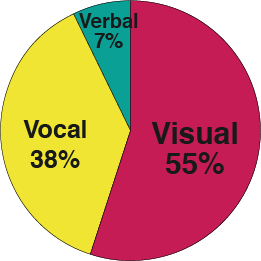
\includegraphics[width=50mm,bb=0 0 261 261]{mehrabian.jpg}}
    \end{center}
    \caption{メラビアンの法則}
    \label{fig:mehrabian}
\end{figure}


\subsection{人との繋がり形成の多様化}
人との繋がりについて書く

\section{本文書の構成}

第1章の最後は、文書全体の構成を大まかに書くとよいらしい。

第\ref{chap:introduction}章では本テンプレートの概要みたいなものを書いた。第\ref{chap:howto}章では、本テンプレートの使い方を説明する。第\ref{chap:latex}章で図表や数式の挿入など代表的な\LaTeX コマンドを解説する。第\ref{chap:conclusion}章では、『序論』で始めたら『結論』で終われと書いた手前書かざるを得ないので、なにか結論らしいことを書く。付録として、テンプレートのサンプルになるように無理矢理ゴミを添付する。
	% 本文1
\chapter{本テンプレートの使い方}
\label{chap:howto}

本章では、本テンプレートの具体的な使用方法を解説する。基本的には、{\tt main.tex} を上から順に修正していけばよいだけ。


\section{テンプレートの構成}

このテンプレートは、表\ref{tb:files}のファイルで構成されている。

\begin{table}[htbp]
  \caption{構成ファイル}
  \label{tb:files}
  \begin{center}\begin{tabular}{c|l}
    \hline
    ファイル名&用途\\\hline\hline
    {\tt main.tex}&メインのファイル。これを編集していく\\\hline
    {\tt thesis.sty}&論文のスタイルを定義したファイル。基本的には手は加えない\\\hline
    {\tt *.tex}&{\tt main.tex}に{\tt include}されるファイル群\\\hline
    {\tt *.eps}&画像ファイル\\\hline
    {\tt main.bib}&参考文献用のBibTeXファイル\\\hline
    {\tt Makefile}&Makefile。次節以降で説明\\\hline
    {\tt .gitignore}&Git用設定ファイル\\\hline
  \end{tabular}\end{center}
\end{table}

\section{コンパイル}
このテンプレートの\LaTeX ファイルをコンパイルしてPDFファイルを生成するには、ターミナルを開いて以下のようにする。

\begin{itembox}[l]{コマンド実行例}
\begin{verbatim}
% make
\end{verbatim}
\end{itembox}

こうすることで、\verb|platex|コマンド、\verb|pbibtex|コマンド、\verb|platex|コマンド2回、\verb|dvipdfmx|コマンドが全て実行され、{\tt main.pdf}が生成される。

コンパイルによって生成されたファイルを全て消すには、以下のようにする。

\begin{itembox}[l]{コマンド実行例}
\begin{verbatim}
% make clean
\end{verbatim}
\end{itembox}

\section{設定}

以下、{\tt main.tex}に対して行うべき設定を、このファイルの中に書いてある順に沿って説明する。

\subsection{論文全体の言語の設定}
\label{sec:lang}

\begin{itembox}[l]{{\tt main.tex}}
\begin{verbatim}
\japanesetrue	% 論文全体を日本語で書く(英語で書くならコメントアウト)
\end{verbatim}
\end{itembox}

ここでは論文全体の言語を設定する。日本語に設定すれば、『章』『目次』『謝辞』などが日本語で出力されて、行頭のインデントなども日本語の仕様になる。英語にした場合は、これらはそれぞれ『Chapter』『Table of Contents』『Acknowledgment』な体裁になる。インデントも行間も、英語用の設定が適用される。

\verb|\japanesetrue| をコメントアウトしなければ日本語に、コメントアウトすれば英語に設定される。


\subsection{余白の設定}

\begin{itembox}[l]{{\tt main.tex}}
\begin{verbatim}
\bindermode	% バインダ用余白設定
\end{verbatim}
\end{itembox}

このテンプレートの出力はA4用紙。ここではこれの四辺の余白を設定する。

最終的にバインダーで綴じて提出する場合、余白を左右対称にしてしまうと、見かけ上のバランスがとても悪くなる。これを解消するため、あらかじめ左側の余白を大きく取っておく。

\verb|\bindermode| をコメントアウトしなければ左綴じ用の余白に、コメントアウトすれば左右対称の余白に設定される。

両面印刷の場合、偶数ページと奇数ページで余白を広くとるべき側が違うので、\verb|documentclass| でこれを設定する。

\begin{itembox}[l]{{\tt main.tex}}
\begin{verbatim}
% 両面印刷の場合。余白を綴じ側に作って右起こし。
\documentclass[a4j,twoside,openright,11pt]{jreport}
% 片面印刷の場合。
%\documentclass[a4j,11pt]{jreport}
\end{verbatim}
\end{itembox}

両面印刷の場合は \verb|twoside| を使用する。\verb|openright| を使うと章のはじまりが必ず右側のページに来るようになる。

\subsection{論文情報の設定}
\label{sec:meta}

\begin{itembox}[l]{{\tt main.tex}}
\begin{verbatim}
% 日本語情報(必要なら)
\jclass  {修士論文}                             % 論文種別
\jtitle    {修士論文用 \LaTeX\ テンプレート}    % タイトル。改行する場合は\\を入れる
\juniv    {慶應義塾大学大学院}                  % 大学名
\jfaculty  {政策・メディア研究科}               % 学部、学科
\jauthor  {ほげ山 ふう助}                       % 著者
\jhyear  {24}                                   % 平成○年度
\jsyear  {2012}                                 % 西暦○年度
\jkeyword  {\LaTeX、テンプレート、修士論文}     % 論文のキーワード
\jproject{インタラクションデザインプロジェクト} %プロジェクト名
\jdate{2013年1月}

% 英語情報(必要なら)
\eclass  {Master's Thesis}                            % 論文種別
\etitle    {A \LaTeX Template for Master Thesis}      % タイトル。改行する場合は\\を入れる
\euniv  {Keio University}                             % 大学名
\efaculty  {Graduate School of Media and Governance}  % 学部、学科
\eauthor  {Fusuke Hogeyama}                           % 著者
\eyear  {2012}                                        % 西暦○年度
\ekeyword  {\LaTeX, Templete, Master Thesis}          % 論文のキーワード
\eproject{Interaction Design Project}                 %プロジェクト名
\edate{January 2013}
\end{verbatim}
\end{itembox}

ここでは論文のタイトルや著者の氏名などのメタデータを記述する。ここで書いたデータは、表紙とアブストラクトのページに使われる。必ずしも日本語と英語の両方を設定しなければいけないわけではなくて、自分が必要とする方だけ記述すればよい。

タイトルが長過ぎる場合は、表紙やアブストラクトのページでは自動で折り返して出力される。もし改行位置を自分で指定したい場合は、その場所に \verb|\\| を入力する。


\section{出力}

\verb|\begin{document}| から \verb|\end{document}| に記述した部分が、実際に{\tt DVI}(最終的には{\tt PDF})ファイルとして出力される。

\subsection{外部ファイルの読み込み({\tt include})}

出力部分の具体的な説明の前に、外部ファイルを読み込む方法を説明する。

\verb|\begin{document}| から \verb|\end{document}| の間では、\verb|\include| コマンドを使うことで、別の {\tt *.tex} ファイルを読み込ませられる。

\begin{itembox}[l]{{\tt include}しない場合}
\begin{itembox}[l]{{\tt main.tex}}
\begin{verbatim}
\begin{document}
  \begin{jabstract}
  ほげほげ
  \end{jabstract}
\end{document}
\end{verbatim}
\end{itembox}
\end{itembox}

\begin{itembox}[l]{{\tt include}する場合}
\begin{minipage}{0.5\hsize}
\begin{itembox}[l]{{\tt main.tex}}
\begin{verbatim}
\begin{document}
\include{01} % 01.texをinclude
\end{document}
\end{verbatim}
\end{itembox}
\end{minipage}
\begin{minipage}{0.5\hsize}
\begin{itembox}[l]{{\tt 01.tex}}
\begin{verbatim}
\begin{jabstract}
ほげほげ
\end{jabstract}
\end{verbatim}
\end{itembox}
\end{minipage}
\end{itembox}

{\tt include}しない場合とする場合を比較するとこのとおり。どちらも出力結果は一緒。{\tt include}する場合は、読み込ませたい箇所に、読み込ませたい{\tt *.tex}ファイルの名前を、拡張子を除いて \verb|\include| コマンドで書けばよい。

\verb|\include| コマンドを用いるか用いないかは、たぶん文書量や個人の好みに依る。例えば章ごとに別のファイルにしておけば、修正箇所を探すときの手間が多少は省けるかもしれない。Gitで人と共有しつつ校正を頼むときにもファイルが分かれていたほうがコンフリクトを起こしにくい。


\subsection{表紙の出力}

\begin{itembox}[l]{{\tt main.tex}}
\begin{verbatim}
\ifjapanese
  \jmaketitle    % 表紙(日本語)
\else
  \emaketitle    % 表紙(英語)
\fi
\end{verbatim}
\end{itembox}

最初に、表紙を出力する。

\verb|\jmaketitle| が実行されると日本語の表紙が、\verb|\emaketitle| が実行されると英語の表紙がそれぞれ出力される。日本語の表紙には、第\ref{sec:meta}節で設定したうちの日本語の情報が、英語の表紙には同節で設定したうち英語の情報が、それぞれ参照されて、表記される。

デフォルトでは第\ref{sec:lang}説で設定した言語の表紙のみが出力されるようになっている。

\subsection{アブストラクトの出力}

\begin{itembox}[l]{{\tt main.tex}}
\begin{verbatim}
\include{00_abstract}	% アブストラクト。要独自コマンド、include先参照のこと
\end{verbatim}
\end{itembox}

表紙の次は、アブストラクト。

アブストラクトを出力するには、出力したい位置に、指定のコマンドを用いて文章を書き下せばよい。{\tt main.tex}に直接書いてもよいし、先述した \verb|\include| コマンドを利用して{\tt include}してもよい。

\verb|\begin{jabstract}| から \verb|\end{jabstract}| の間に書いた文章が日本語のアブストラクトとして、\verb|\begin{eabstract}| から \verb|\end{eabstract}| の間に書いた文章が英語のアブストラクトとして、それぞれ独立したページに出力される。

アブストラクトのページには、論文のタイトルやキーワードなどが、第\ref{sec:meta}節で設定した情報をもとにして自動で表記される。

日本語か英語のどちらか一方のみでよい場合は、不要な言語の方のコマンドを削除すればよい。これは、\verb|\begin| と \verb|\end| というコマンド自身も含めて削除する、ということで、\verb|\begin| と \verb|\end| の間を空っぽにするという意味ではないので注意。



\subsection{目次類の出力}
\label{sec:toc}

\begin{itembox}[l]{{\tt main.tex}}
\begin{verbatim}
\tableofcontents	% 目次
\listoffigures		% 表目次
\listoftables		% 図目次
\end{verbatim}
\end{itembox}

アブストラクトの次に、目次。文書の目次、図の目次、表の目次の三種類。

目次類を出力するには、出力したい位置に指定のコマンドを書けばよい。

これらのコマンドは、コンパイル時点での一時ファイル\footnote{{\tt *.toc}、{\tt *.lof}、{\tt *.lot}}の情報を、目次として体裁を整えて出力するもの。一時ファイルは、\verb|\begin{document}| から \verb|\end{document}| の間の章や節、図や表をコンパイルするときに、ついでに情報を取得しておいて生成される。

つまり気をつけなければいけないのは、コンパイルを一回しただけでは、一時ファイルが最新の状態に更新されるだけで、肝心の目次は正しい情報では出力されないということ。目次類を正しい情報で出力するには、最低二回のコンパイルが必要。一回目のコンパイルで一時ファイルが最新の情報に更新されて、二回目のコンパイルで初めて、その最新の一時ファイルの情報をもとに目次が出力される。

だから、文書に何らかの修正をして保存したあとは、最低でも二回、連続してコンパイルしないといけないことに注意する。

図や表を一つも使用していない場合は、目次名のみが書かれた空白のページが出力される。もしこれが不要な場合は、該当するコマンドをコメントアウトすればよい。


\subsection{本文の出力}

\begin{itembox}[l]{{\tt main.tex}}
\begin{verbatim}
\include{01}	% 本文1
\include{02}	% 本文2
\include{03}	% 本文3
\include{04}	% 本文4
\end{verbatim}
\end{itembox}

目次に続いて、論文のメイン、本文を記述する。アブストラクトと同様で、{\tt main.tex}に直接書くか、\verb|\include| コマンドを利用して別に用意したファイルを{\tt include}する。

本文の書き方は、第\ref{chap:latex}章で詳しく説明する。


\subsection{謝辞の出力}

\begin{itembox}[l]{{\tt main.tex}}
\begin{verbatim}
\include{90_acknowledgment}	% 謝辞。要独自コマンド、include先参照のこと
\end{verbatim}
\end{itembox}

本文のあとには、謝辞を出力する。\verb|begin{acknowledgment}| から \verb|end{acknowledgment}| の間に書いた文章が、謝辞として独立したページに出力される。アブストラクトや本文と同じで、{\tt main.tex}に直接書いてもよいし、\verb|\include| コマンドを利用して{\tt include}してもよい。


\subsection{参考文献の出力}

\begin{itembox}[l]{{\tt main.tex}}
\begin{verbatim}
\include{91_bibliography}	% 参考文献。要独自コマンド、include先参照のこと
\end{verbatim}
\end{itembox}

謝辞に続いて、参考文献を出力する。

参考文献リストは、\verb|\begin{bib}| から \verb|\end{bib}| の間に、\verb|\bibitem| コマンドを使って書く。

BibTeXを使う場合は、以下のようにする。

\begin{itembox}[l]{{\tt 91\_bibliography.tex}}
\begin{verbatim}
\begin{bib}[100]
\bibliography{main}
\end{bib}
\end{verbatim}
\end{itembox}

こうすると、\verb|main.bib|から使用した参考文献のみを抽出して出力してくれる。\verb|main.bib|の中身は以下のようになっていて、気の利いた論文検索サイトであればBibTeXをコピペできるようになっているので簡単に作れるはず。


\begin{itembox}[l]{{\tt 91\_bibliography.tex}}
\begin{verbatim}
@article{hoge09,
    author  = "ほげ山太郎 and ほげ山次郎",
    yomi    = "ほげやまたろう",
    title   = "ほげほげ理論のHCI分野への応用",
    journal = "ほげほげ学会論文誌",
    volume  = "31",
    number  = "3",
    pages   = "194-201",
    year    = "2009",
}
@inproceedings{hoge08,
    author     = "Taro Hogeyama and Jiro Hogeyama",
    title      = "The Theory of Hoge",
    booktitle  = "The Proceedings of The Hoge Society",
    year       = "2008"
}
\end{verbatim}
\end{itembox}


以下は、BibTeXを使わないで手で書く例。

\begin{itembox}[l]{{\tt 91\_bibliography.tex}}
\begin{verbatim}
@article{hoge09,
    author  = "ほげ山太郎 and ほげ山次郎",
    yomi    = "ほげやまたろう",
    title   = "ほげほげ理論のHCI分野への応用",
    journal = "ほげほげ学会論文誌",
    volume  = "31",
    number  = "3",
    pages   = "194-201",
    year    = "2009",
}
@inproceedings{hoge08,
    author     = "Taro Hogeyama and Jiro Hogeyama",
    title      = "The Theory of Hoge",
    booktitle  = "The Proceedings of The Hoge Society",
    year       = "2008"
}
\end{verbatim}
\end{itembox}


英語の文献の場合、慣例的に書誌名をイタリック体にすることが多いらしい。

\begin{itembox}[l]{{\tt 91\_bibliography.tex}}
\begin{verbatim}
\begin{bib}[100]
\begin{thebibliography}{#1}
% \bibitem{参照用名称}
%   著者名:
%   \newblock 文献名,
%   \newblock 書誌情報,出版年.

\bibitem{hoge09}
  ほげ山太郎,ほげ山次郎:
  \newblock ほげほげ理論のHCI分野への応用,
  \newblock ほげほげ学会論文誌,Vol.31,No.3,pp.194-201,2009.

\bibitem{hoge08}
  Taro Hogeyama, Jiro Hogeyama:
  \newblock The Theory of Hoge,
  \newblock {\it The Proceedings of The Hoge Society}, 2008.
\end{thebibliography}
\end{bib}
\end{verbatim}
\end{itembox}

\verb|\bibitem| コマンド中、参照用名称は、本文から参考文献を参照するときに使うので、忘れずに書いておく。参照文献を本文中に参照するときには、\verb|\cite{参照用名称}| のように書けばよい。例えば、この文の末尾には \verb|\cite{hoge09}| と書いてあるので、自動で対応する番号が振られる\cite{hoge09}\cite{hoge08}。

参考文献リストの番号付けと、本文で参照したときの番号の挿入は、全部が自動で行われる。ただしこれも、第\ref{sec:toc}節で説明した目次の出力と同じで、一時ファイルを生成してからの挿入なので、正しく出力するには最低でも二回のコンパイルが必要。BibTeXを使用する場合は、\verb|platex|コマンドのあと\verb|pbibtex|コマンドを実行し、さらに2回\verb|platex|コマンドを実行するといいらしい。



\subsection{付録の出力}

\begin{itembox}[l]{{\tt main.tex}}
\begin{verbatim}
\appendix
\include{92_appendix}		% 付録
\end{verbatim}
\end{itembox}

必要であれば、論文の最後には付録を出力する。

\verb|\appendix| コマンド以降に書いたものは、すべて付録として扱われる。付録部分の書き方は通常の本文とまったく同じで、\verb|\appendix| コマンド以降に書くだけで勝手に付録用の体裁で出力される。
	% 本文2
\chapter{\LaTeX の書き方}
\label{chap:latex}

この章では、よく使う\LaTeX のコマンドを説明する。足りない部分はぐぐればだいたいわかると思う。最初に書いておくと、数式を書く方法は、ぼく自身使わなかったので書いていない。ぼくのいた研究室でごりごり数式をたくさん書く必要のあるひとは、研究の種類からするとあまり居ない気がする。

\section{主なコマンド}

\subsection{章と節}

文書構造を明確にする大事なもの。目次はこれらのコマンドをもとに作られる。例えば、この第\ref{chap:latex}章の冒頭部分はこのようなソースで書かれている。

\begin{itembox}[l]{{\tt 03.tex}}
\begin{verbatim}
\chapter{\LaTeX の書き方}
\label{chap:latex}

この章では、よく使う\LaTeX のコマンドを説明する。(略)

\section{主なコマンド}

\subsection{章と節}

文書構造を明確にする大事なもの。目次はこれらのコマンドをもとに作られる。例えば、この第\ref{chap:latex}章の冒頭部分はこのようなソースで書かれている。
\end{verbatim}
\end{itembox}

章は \verb|\chapter{見出し}|、節は \verb|\section{見出し}|、小節は \verb|\subsection{見出し}|、小々節は \verb|\subsubsection{見出し}| を使う。表\ref{tb:chap}に一覧する。

\begin{table}[htbp]
  \caption{章と節のコマンド}
  \label{tb:chap}
  \begin{center}\begin{tabular}{c|c}
    \hline
    コマンド&用途\\\hline\hline
    \verb|\chapter{見出し}|&章\\\hline
    \verb|\section{見出し}|&節\\\hline
    \verb|\subsection{見出し}|&小節\\\hline
    \verb|\subsubsection{見出し}|&小々節\\\hline
    \end{tabular}\end{center}
\end{table}

\subsubsection{小々節見出しサンプルその1}

小々節は上のように \verb|\subsubsection{タイトル}| で書けるけれど、あまり文書の階層構造が深いことは望ましくないので、多用しなければならないようなら文書構造を見直したほうがよいと思う。

\subsubsection{小々節見出しサンプルその2}

小々節は、章や節、小節のように {\tt N.N.N} といった番号ではなくて、括弧付きの番号で出力される。かつ、目次には出力されない。

\subsection{図}

図は次のように出力される(図\ref{fig:sample1})。

\begin{figure}[htbp]
    \begin{center}
       \fbox{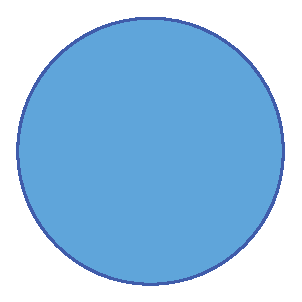
\includegraphics[width=50mm]{image.eps}}
    \end{center}
    \caption{図の例}
    \label{fig:sample1}
\end{figure}

ソースでは次のように記述している。

\begin{itembox}[l]{{\tt 03.tex}}
\begin{verbatim}
図は次のように出力される(図\ref{fig:sample1})。

\begin{figure}[htbp]
    \begin{center}
       \fbox{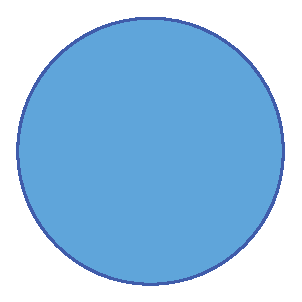
\includegraphics[width=40mm]{image.eps}}
    \end{center}
    \caption{図の例}
    \label{fig:sample1}
\end{figure}
\end{verbatim}
\end{itembox}

\verb|\begin{figure}[htbp]|  の{\tt htbp}は、表示位置の優先順位の設定。基本的に\LaTeX では、図の挿入位置は強制的には指定できない。いくつか候補を指定しておくと、候補のなかの優先度の高い順に、図を入れられるスペースがあるかどうかを調べて、入れられればそこに、入れられなければ次の候補のスペースを調べる、という処理が行われる。{\tt h}はこのコマンドを書いたその場所に、{\tt t}はページの一番上に、{\tt b}はページの一番下に、{\tt p}は画像だけ別ページに、それぞれ配置する。基本的には{\tt htbp}のように全部書いておけば問題ない。

\verb|\includegraphics| コマンドで、図のサイズと挿入するファイルを指定する。上の例ではサイズは {\tt width=50mm} として幅を指定したけれど、ここは他にも {\tt height=30mm} として高さを指定してもよいし、{\tt scale=0.5} として拡大率を指定してもよい。画像は最近の \LaTeX 環境であれば{\tt *.eps}以外でも使える。ただし、{\tt bb} (Bounding Box) として画像の大きさを指定する必要があることも多い。
以下はJPEG画像を使用する例。

\begin{itembox}[l]{{\tt 03.tex}}
\begin{verbatim}
\begin{figure}[htbp]
    \begin{center}
       \fbox{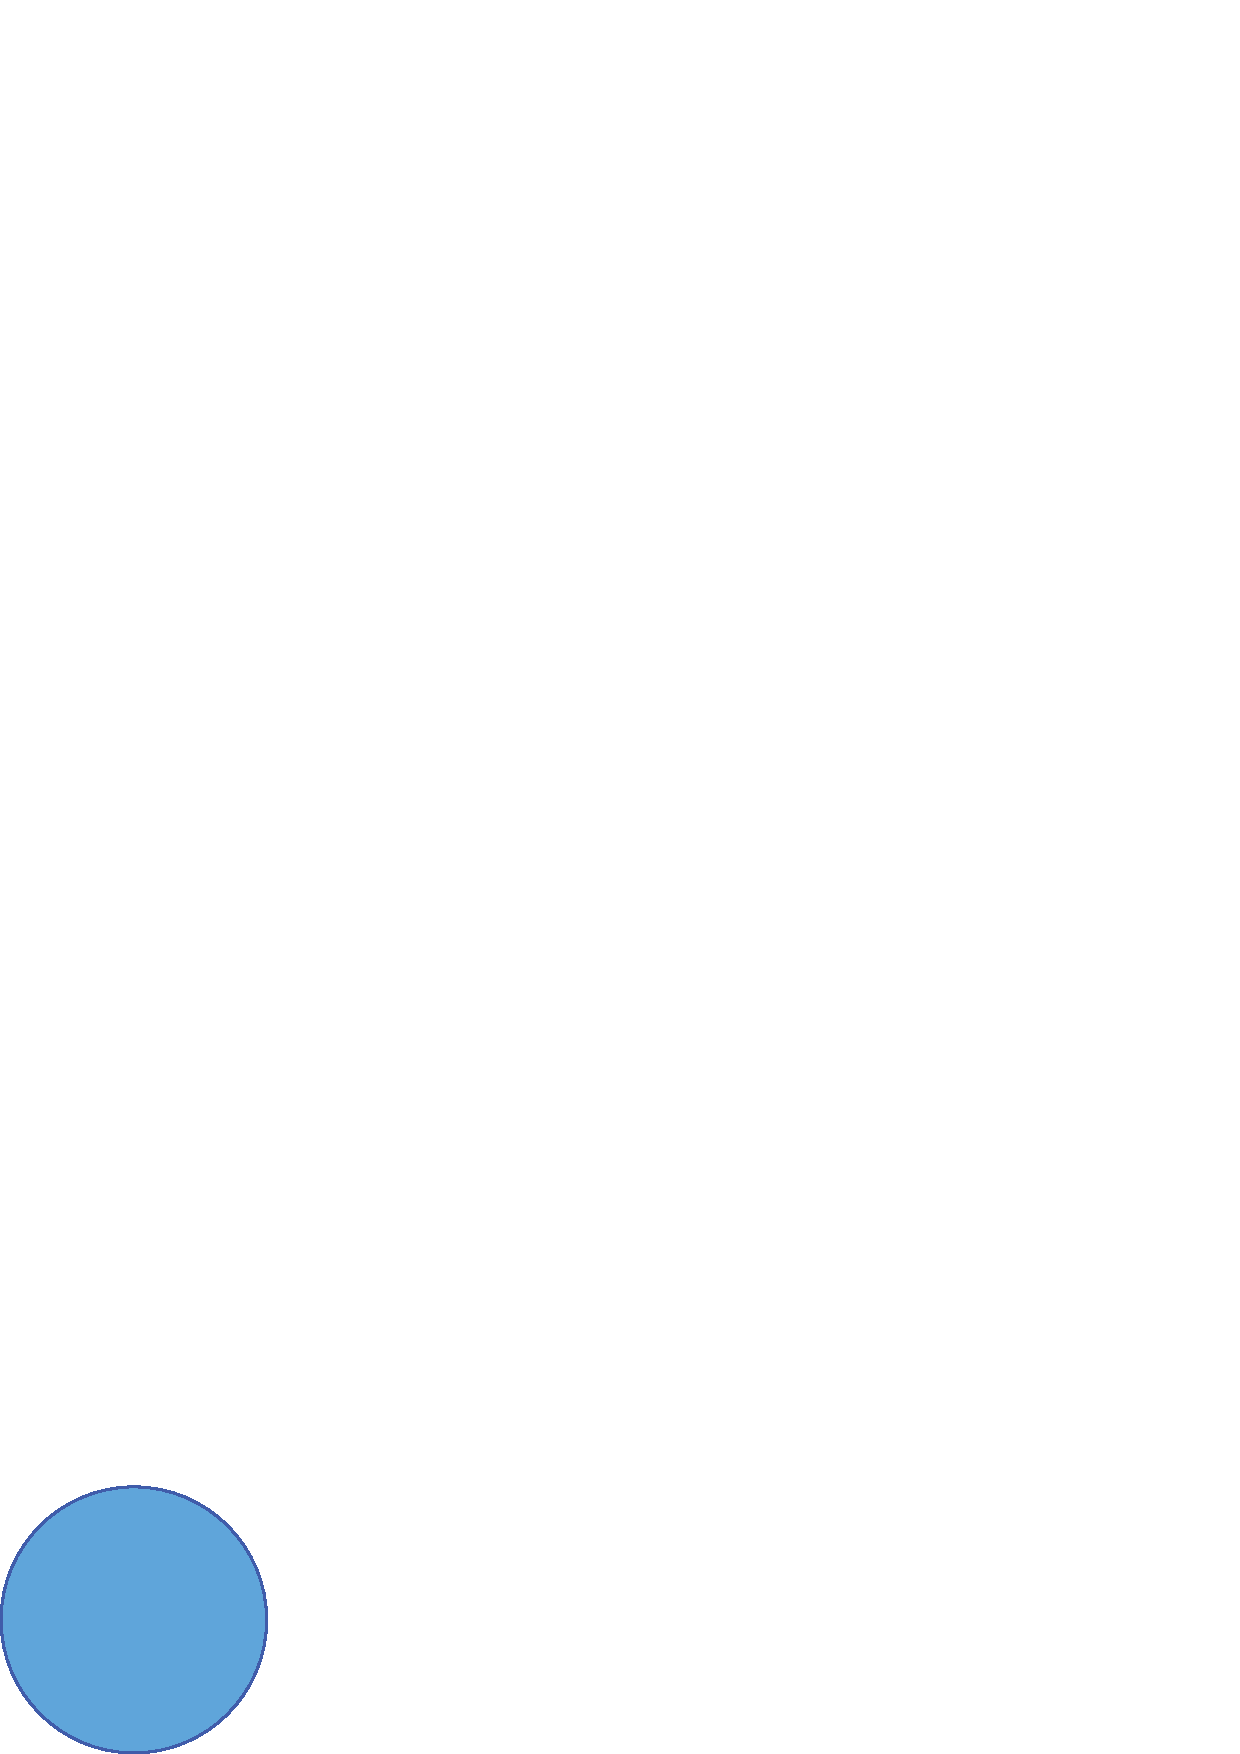
\includegraphics[width=40mm,bb=0 0 640 480]{image.jpg}}
    \end{center}
    \caption{図の例}
    \label{fig:sample1}
\end{figure}
\end{verbatim}
\end{itembox}

bbの指定は、上記のように{\tt *.tex} ファイルの中で指定してもいいが、
{\tt *.bb}ファイルを作っておく方法もある。
ターミナルで{\tt ebb}コマンドを使用すると{\tt *.bb}ファイルを簡単に作れる。


\begin{itembox}[l]{ebbコマンドの例}
\begin{verbatim}
% ebb image.jpg
\end{verbatim}
\end{itembox}


\verb|\includegraphics| を \verb|\fbox| に入れると、画像に枠を付けられる。

\verb|\caption| コマンドで図の見出しを指定できる。図の見出しは、図の下に表記するので注意。ここで指定した見出しが、図の目次に表示される。

\verb|\label| コマンドでは図の参照用ラベルを設定できる。本文中、\verb|\ref| コマンドで参照用ラベルを指定すると、対応した図の番号が自動的に挿入される。これも目次や参考文献と同様、最低二回のコンパイルが必要なので注意。

図を二つ横に並べたい場合は、次のように書く(図\ref{fig:sample2}、図\ref{fig:sample3})。

\begin{figure}[htbp]
  \begin{minipage}{0.5\hsize}
    \begin{center}
       \fbox{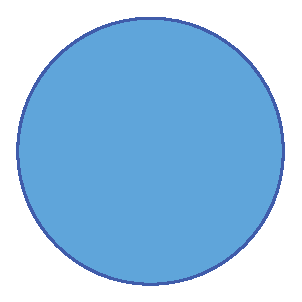
\includegraphics[width=40mm]{image.eps}}
    \end{center}
    \caption{図を並べる例1}
    \label{fig:sample2}
  \end{minipage}
  \begin{minipage}{0.5\hsize}
    \begin{center}
       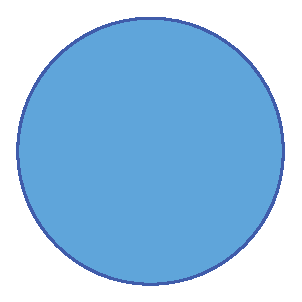
\includegraphics[width=40mm]{image.eps}
    \end{center}
    \caption{図を並べる例2、枠なし}
    \label{fig:sample3}
  \end{minipage}
\end{figure}

\begin{itembox}[l]{{\tt 03.tex}}
\begin{verbatim}
図を二つ横に並べたい場合は、次のように書く(図\ref{fig:sample2}、図\ref{fig:sample3})。

\begin{figure}[htbp]
  \begin{minipage}{0.5\hsize}
    \begin{center}
       \fbox{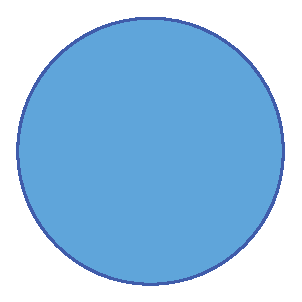
\includegraphics[width=40mm]{image.eps}}
    \end{center}
    \caption{図を並べる例1}
    \label{fig:sample2}
  \end{minipage}
  \begin{minipage}{0.5\hsize}
    \begin{center}
       \fbox{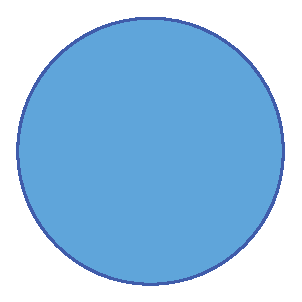
\includegraphics[width=40mm]{image.eps}}
    \end{center}
    \caption{図を並べる例2}
    \label{fig:sample3}
  \end{minipage}
\end{figure}
\end{verbatim}
\end{itembox}


\subsection{表}

表は次のように出力される(表\ref{tb:sample1})。

\begin{table}[htbp]
  \caption{表の例}
  \label{tb:sample1}
  \begin{center}
  \begin{tabular}{l|c|r}
    \hline
    種類	&味&評価\\\hline\hline
    ドラ焼き&甘い&好き\\\hline
    メロンパン&カリもふ&好き\\\hline
    クリームパン&神&すごく好き\\\hline
  \end{tabular}\end{center}
\end{table}

ソースでは次のようになっている。

\begin{itembox}[l]{{\tt 03.tex}}
\begin{verbatim}
表は次のように出力される(表\ref{tb:sample1})。

\begin{table}[htbp]
  \caption{表の例}
  \label{tb:sample1}
  \begin{center}
  \begin{tabular}{l|c|r}
    \hline
    種類	&味&評価\\\hline\hline
    ドラ焼き&甘い&好き\\\hline
    メロンパン&カリもふ&好き\\\hline
    クリームパン&神&すごく好き\\\hline
  \end{tabular}\end{center}
\end{table}
\end{verbatim}
\end{itembox}

{\tt htbp}や \verb|\caption| と \verb|\label| は図と同様。ただし表のタイトルは表の上に書く。

\verb|\begin{tabular}{l|{\tt \textbar}{\tt c}{\tt \textbar}\verb|r}|で横方向のセルを指定する。{\tt c}は中央揃え、{\tt l}は左揃え、{\tt r}は右揃えのセルを作る。{\tt \textbar}は垂直方向の罫線を表す。{\tt c}か{\tt l}か{\tt r}を必要なセルの数だけ並べて、セルの間に罫線が必要なら{\tt \textbar}を入れればよい。

セルの中の文字は、{\tt \&}で区切って並べる。行と行は \verb|\\| で区切る。水平方向の罫線が必要なら、\verb|\hline| を書く。

水平方向や垂直方向のセルの結合もできる。例を示すので、くわしくはぐぐろう。説明がめんどう。\verb|\multirow|、\verb|\multicolumn|、\verb|\cline| を使うとできる。

\begin{table}[htbp]
  \caption{セルを結合した例}
  \label{tb:sample2}
  \begin{center}
  \begin{tabular}{c|c|c}
    \hline
    ほげ&ふー&ばー\\\hline\hline
    \multirow{2}{*}{ほげほげ}&\multicolumn{2}{c}{ふーふー} \\\cline{2-3}
    &ふーふーふー&ばーばーばー\\\hline
  \end{tabular}
  \end{center}
\end{table}

\begin{itembox}[l]{{\tt 03.tex}}
\begin{verbatim}
\begin{table}[htbp]
  \caption{セルを結合した例}
  \label{tb:sample2}
  \begin{center}
  \begin{tabular}{c|c|c}
    \hline
    ほげ&ふー&ばー\\\hline\hline
    \multirow{2}{*}{ほげほげ}&\multicolumn{2}{c}{ふーふー} \\\cline{2-3}
    &ふーふーふー&ばーばーばー\\\hline
  \end{tabular}
  \end{center}
\end{table}
\end{verbatim}
\end{itembox}


\subsection{脚注}

脚注は \verb|\footnote| コマンドを使う。例えばこんな感じ\footnote{ページの下に小さく説明を出せる}。

\begin{itembox}[l]{{\tt 03.tex}}
\begin{verbatim}
例えばこんな感じ\footnote{ページの下に小さく説明を出せる}。
\end{verbatim}
\end{itembox}

\section{その他のコマンド}

ぐぐる\footnote{http://www.google.co.jp/}。

特殊なことは何もしていないテンプレートなので、ぐぐって出たことはだいたいそのまま何でも使える。

あるいは、このファイル自体も\LaTeX で書かれているわけだから、これの{\tt *.tex}を見るのもよいかもしれない。


	% 本文3
\chapter{結論}
\label{chap:conclusion}

この章では、結論らしいことをかく。

\section{まとめ}

\LaTeX の環境さえあればスタンダードな体裁の論文がたぶんだれでも作れる程度のテンプレートにはなっているはず。がんばって卒業しよう。


\section{大事なこと}

箇条書きで列挙する。

\begin{itemize}
 \item ぐぐる。これは単なる\LaTeX だし、\LaTeX はもう枯れた技術だから、調べれば文献はいくらでもある。
 \item 先生を頼る。
 \item 単位をきちんとる。
 \item 卒業する。
\end{itemize}


	% 本文4
\end{verbatim}
\end{itembox}

目次に続いて、論文のメイン、本文を記述する。アブストラクトと同様で、{\tt main.tex}に直接書くか、\verb|\include| コマンドを利用して別に用意したファイルを{\tt include}する。

本文の書き方は、第\ref{chap:latex}章で詳しく説明する。


\subsection{謝辞の出力}

\begin{itembox}[l]{{\tt main.tex}}
\begin{verbatim}
\begin{acknowledgment}
謝辞!!!\\
感謝の言葉を述べる方々はたくさんいらっしゃる...\\
アブストラクトを書いて, 本当の締めで書く.\\
RGの先生方, 仁さん, 大越さん, 陳さん, 柘植さん, 友隆さんを始めとする中澤研究室のファカルティーの方々\\
kgの垣根を超えた大学院の先輩方\\
wataruさん, isokichiさん, drgnmanさん, iphooさんの博士の先輩方,\\
eigenさん,quantan,mokkyさん, ozaさんの修士の先輩方.\\
そしてなにより親のshinsan.\\
兄妹のyuniを始めとする,kg-HAISYSの同期・後輩たち, 中澤研究室の同期後輩たち\\
野中先生のお名前もいれたい, 野中研の研究室メンバーも.\\
そして両親に挨拶をして論文を終わる予定\\

\end{acknowledgment}
	% 謝辞。要独自コマンド、include先参照のこと
\end{verbatim}
\end{itembox}

本文のあとには、謝辞を出力する。\verb|begin{acknowledgment}| から \verb|end{acknowledgment}| の間に書いた文章が、謝辞として独立したページに出力される。アブストラクトや本文と同じで、{\tt main.tex}に直接書いてもよいし、\verb|\include| コマンドを利用して{\tt include}してもよい。


\subsection{参考文献の出力}

\begin{itembox}[l]{{\tt main.tex}}
\begin{verbatim}

\begin{bib}[100]
% BibTeXを使う場合
\bibliography{main}

%\begin{thebibliography}{#1}
%
%  \bibitem{参照用名称}
%    著者名: 
%    \newblock 文献名,
%    \newblock 書誌情報,出版年.
%
% \bibitem{hoge09}
%   ほげ山太郎,ほげ山次郎:
%   \newblock ほげほげ理論のHCI分野への応用,
%   \newblock ほげほげ学会論文誌,Vol.31,No.3,pp.194-201,2009.
% 
% \bibitem{hoge08}
%   Taro Hogeyama, Jiro Hogeyama:
%   \newblock The Theory of Hoge,
%   \newblock {\it The Proceedings of The Hoge Society}, 2008.
%	
%\end{thebibliography}

\end{bib}
	% 参考文献。要独自コマンド、include先参照のこと
\end{verbatim}
\end{itembox}

謝辞に続いて、参考文献を出力する。

参考文献リストは、\verb|\begin{bib}| から \verb|\end{bib}| の間に、\verb|\bibitem| コマンドを使って書く。

BibTeXを使う場合は、以下のようにする。

\begin{itembox}[l]{{\tt 91\_bibliography.tex}}
\begin{verbatim}
\begin{bib}[100]
\bibliography{main}
\end{bib}
\end{verbatim}
\end{itembox}

こうすると、\verb|main.bib|から使用した参考文献のみを抽出して出力してくれる。\verb|main.bib|の中身は以下のようになっていて、気の利いた論文検索サイトであればBibTeXをコピペできるようになっているので簡単に作れるはず。


\begin{itembox}[l]{{\tt 91\_bibliography.tex}}
\begin{verbatim}
@article{hoge09,
    author  = "ほげ山太郎 and ほげ山次郎",
    yomi    = "ほげやまたろう",
    title   = "ほげほげ理論のHCI分野への応用",
    journal = "ほげほげ学会論文誌",
    volume  = "31",
    number  = "3",
    pages   = "194-201",
    year    = "2009",
}
@inproceedings{hoge08,
    author     = "Taro Hogeyama and Jiro Hogeyama",
    title      = "The Theory of Hoge",
    booktitle  = "The Proceedings of The Hoge Society",
    year       = "2008"
}
\end{verbatim}
\end{itembox}


以下は、BibTeXを使わないで手で書く例。

\begin{itembox}[l]{{\tt 91\_bibliography.tex}}
\begin{verbatim}
@article{hoge09,
    author  = "ほげ山太郎 and ほげ山次郎",
    yomi    = "ほげやまたろう",
    title   = "ほげほげ理論のHCI分野への応用",
    journal = "ほげほげ学会論文誌",
    volume  = "31",
    number  = "3",
    pages   = "194-201",
    year    = "2009",
}
@inproceedings{hoge08,
    author     = "Taro Hogeyama and Jiro Hogeyama",
    title      = "The Theory of Hoge",
    booktitle  = "The Proceedings of The Hoge Society",
    year       = "2008"
}
\end{verbatim}
\end{itembox}


英語の文献の場合、慣例的に書誌名をイタリック体にすることが多いらしい。

\begin{itembox}[l]{{\tt 91\_bibliography.tex}}
\begin{verbatim}
\begin{bib}[100]
\begin{thebibliography}{#1}
% \bibitem{参照用名称}
%   著者名:
%   \newblock 文献名,
%   \newblock 書誌情報,出版年.

\bibitem{hoge09}
  ほげ山太郎,ほげ山次郎:
  \newblock ほげほげ理論のHCI分野への応用,
  \newblock ほげほげ学会論文誌,Vol.31,No.3,pp.194-201,2009.

\bibitem{hoge08}
  Taro Hogeyama, Jiro Hogeyama:
  \newblock The Theory of Hoge,
  \newblock {\it The Proceedings of The Hoge Society}, 2008.
\end{thebibliography}
\end{bib}
\end{verbatim}
\end{itembox}

\verb|\bibitem| コマンド中、参照用名称は、本文から参考文献を参照するときに使うので、忘れずに書いておく。参照文献を本文中に参照するときには、\verb|\cite{参照用名称}| のように書けばよい。例えば、この文の末尾には \verb|\cite{hoge09}| と書いてあるので、自動で対応する番号が振られる\cite{hoge09}\cite{hoge08}。

参考文献リストの番号付けと、本文で参照したときの番号の挿入は、全部が自動で行われる。ただしこれも、第\ref{sec:toc}節で説明した目次の出力と同じで、一時ファイルを生成してからの挿入なので、正しく出力するには最低でも二回のコンパイルが必要。BibTeXを使用する場合は、\verb|platex|コマンドのあと\verb|pbibtex|コマンドを実行し、さらに2回\verb|platex|コマンドを実行するといいらしい。



\subsection{付録の出力}

\begin{itembox}[l]{{\tt main.tex}}
\begin{verbatim}
\appendix
\chapter{付録の例}

付録を無理矢理出力させるため、てきとうなことを書く。

\section{ほげ}

コマンドは本文と一緒。

\subsection{ふー}

本文と一緒。

\section{ほげほげ}

本文と一緒。

\subsection{ふーふー}

本文と一緒。
		% 付録
\end{verbatim}
\end{itembox}

必要であれば、論文の最後には付録を出力する。

\verb|\appendix| コマンド以降に書いたものは、すべて付録として扱われる。付録部分の書き方は通常の本文とまったく同じで、\verb|\appendix| コマンド以降に書くだけで勝手に付録用の体裁で出力される。
	% 本文2
\chapter{\LaTeX の書き方}
\label{chap:latex}

この章では、よく使う\LaTeX のコマンドを説明する。足りない部分はぐぐればだいたいわかると思う。最初に書いておくと、数式を書く方法は、ぼく自身使わなかったので書いていない。ぼくのいた研究室でごりごり数式をたくさん書く必要のあるひとは、研究の種類からするとあまり居ない気がする。

\section{主なコマンド}

\subsection{章と節}

文書構造を明確にする大事なもの。目次はこれらのコマンドをもとに作られる。例えば、この第\ref{chap:latex}章の冒頭部分はこのようなソースで書かれている。

\begin{itembox}[l]{{\tt 03.tex}}
\begin{verbatim}
\chapter{\LaTeX の書き方}
\label{chap:latex}

この章では、よく使う\LaTeX のコマンドを説明する。(略)

\section{主なコマンド}

\subsection{章と節}

文書構造を明確にする大事なもの。目次はこれらのコマンドをもとに作られる。例えば、この第\ref{chap:latex}章の冒頭部分はこのようなソースで書かれている。
\end{verbatim}
\end{itembox}

章は \verb|\chapter{見出し}|、節は \verb|\section{見出し}|、小節は \verb|\subsection{見出し}|、小々節は \verb|\subsubsection{見出し}| を使う。表\ref{tb:chap}に一覧する。

\begin{table}[htbp]
  \caption{章と節のコマンド}
  \label{tb:chap}
  \begin{center}\begin{tabular}{c|c}
    \hline
    コマンド&用途\\\hline\hline
    \verb|\chapter{見出し}|&章\\\hline
    \verb|\section{見出し}|&節\\\hline
    \verb|\subsection{見出し}|&小節\\\hline
    \verb|\subsubsection{見出し}|&小々節\\\hline
    \end{tabular}\end{center}
\end{table}

\subsubsection{小々節見出しサンプルその1}

小々節は上のように \verb|\subsubsection{タイトル}| で書けるけれど、あまり文書の階層構造が深いことは望ましくないので、多用しなければならないようなら文書構造を見直したほうがよいと思う。

\subsubsection{小々節見出しサンプルその2}

小々節は、章や節、小節のように {\tt N.N.N} といった番号ではなくて、括弧付きの番号で出力される。かつ、目次には出力されない。

\subsection{図}

図は次のように出力される(図\ref{fig:sample1})。

\begin{figure}[htbp]
    \begin{center}
       \fbox{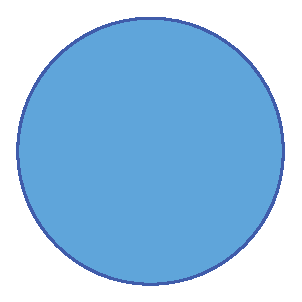
\includegraphics[width=50mm]{image.eps}}
    \end{center}
    \caption{図の例}
    \label{fig:sample1}
\end{figure}

ソースでは次のように記述している。

\begin{itembox}[l]{{\tt 03.tex}}
\begin{verbatim}
図は次のように出力される(図\ref{fig:sample1})。

\begin{figure}[htbp]
    \begin{center}
       \fbox{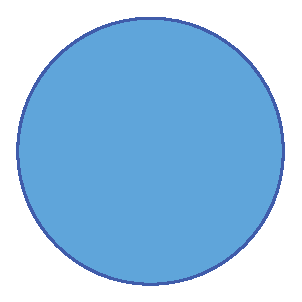
\includegraphics[width=40mm]{image.eps}}
    \end{center}
    \caption{図の例}
    \label{fig:sample1}
\end{figure}
\end{verbatim}
\end{itembox}

\verb|\begin{figure}[htbp]|  の{\tt htbp}は、表示位置の優先順位の設定。基本的に\LaTeX では、図の挿入位置は強制的には指定できない。いくつか候補を指定しておくと、候補のなかの優先度の高い順に、図を入れられるスペースがあるかどうかを調べて、入れられればそこに、入れられなければ次の候補のスペースを調べる、という処理が行われる。{\tt h}はこのコマンドを書いたその場所に、{\tt t}はページの一番上に、{\tt b}はページの一番下に、{\tt p}は画像だけ別ページに、それぞれ配置する。基本的には{\tt htbp}のように全部書いておけば問題ない。

\verb|\includegraphics| コマンドで、図のサイズと挿入するファイルを指定する。上の例ではサイズは {\tt width=50mm} として幅を指定したけれど、ここは他にも {\tt height=30mm} として高さを指定してもよいし、{\tt scale=0.5} として拡大率を指定してもよい。画像は最近の \LaTeX 環境であれば{\tt *.eps}以外でも使える。ただし、{\tt bb} (Bounding Box) として画像の大きさを指定する必要があることも多い。
以下はJPEG画像を使用する例。

\begin{itembox}[l]{{\tt 03.tex}}
\begin{verbatim}
\begin{figure}[htbp]
    \begin{center}
       \fbox{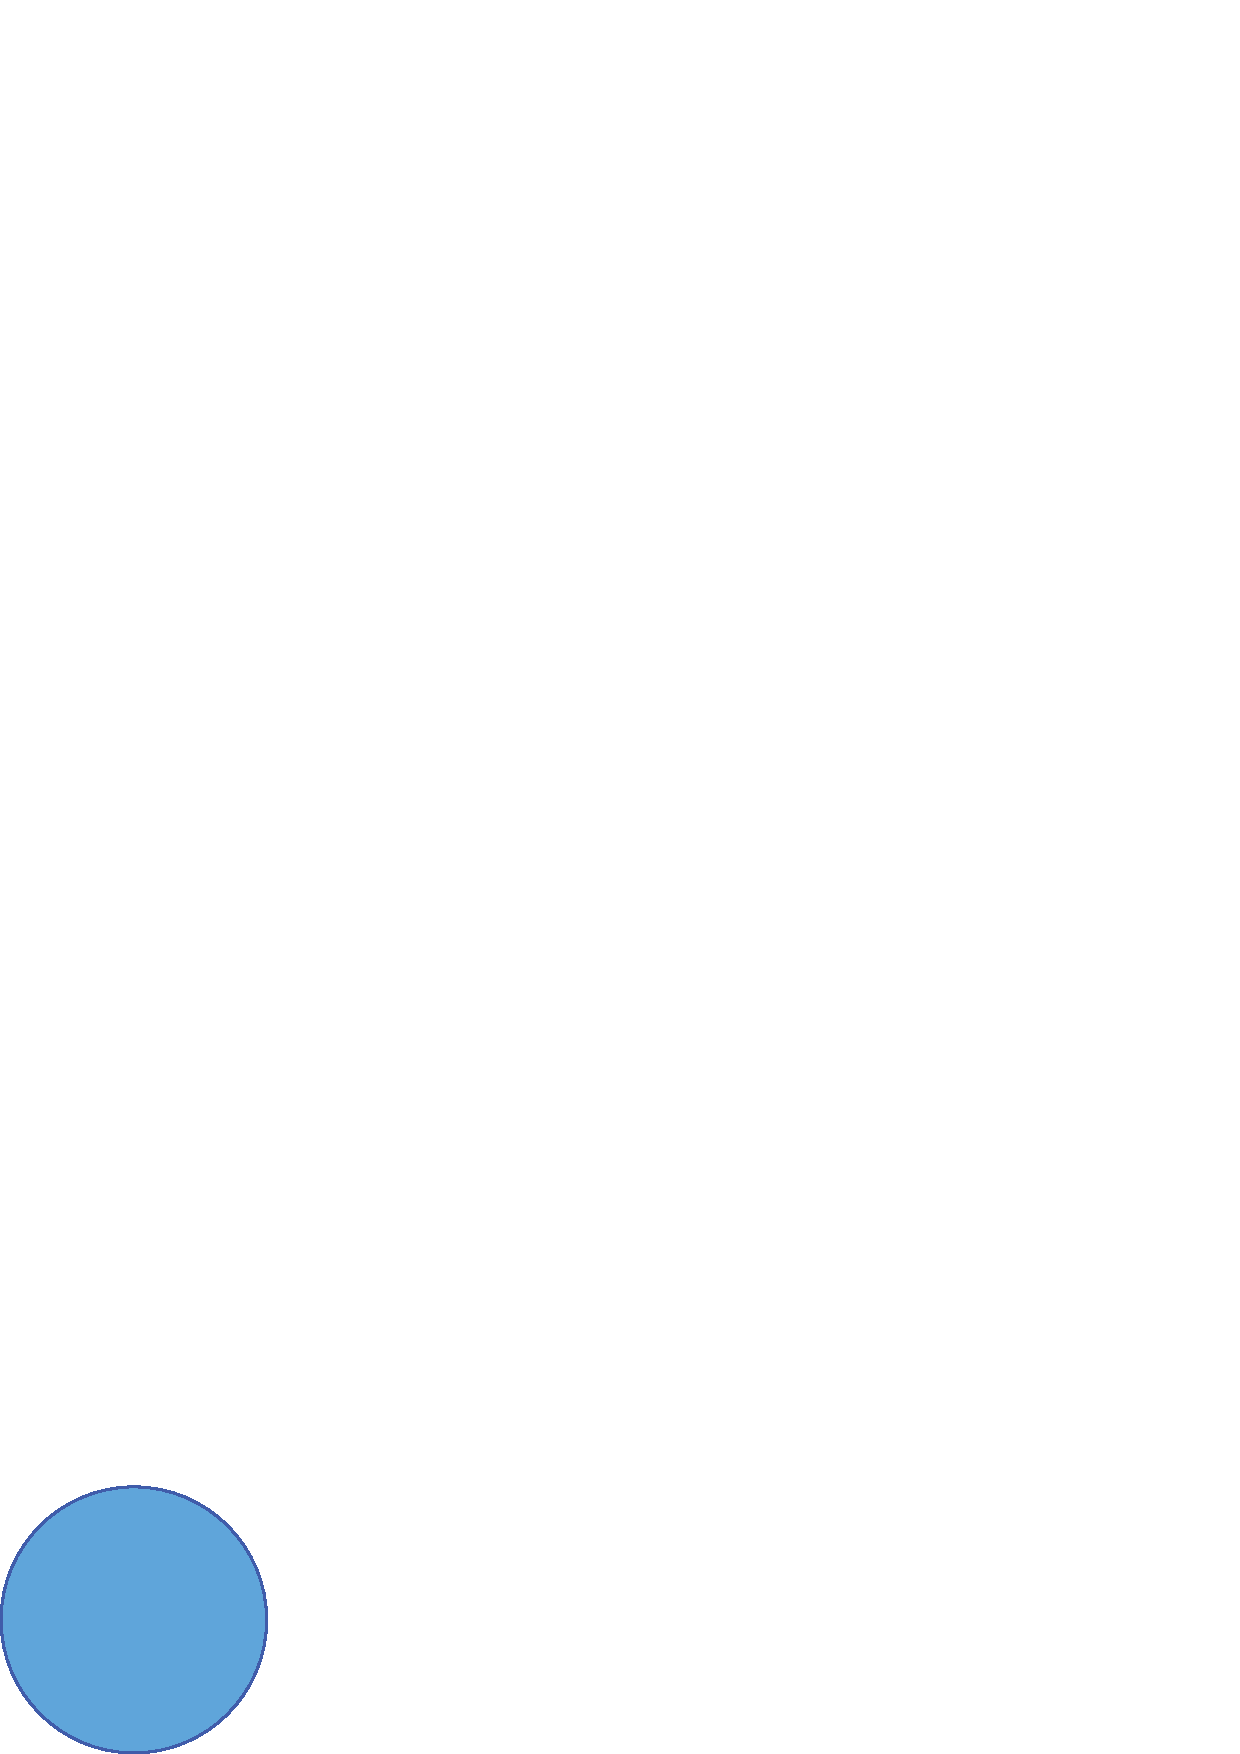
\includegraphics[width=40mm,bb=0 0 640 480]{image.jpg}}
    \end{center}
    \caption{図の例}
    \label{fig:sample1}
\end{figure}
\end{verbatim}
\end{itembox}

bbの指定は、上記のように{\tt *.tex} ファイルの中で指定してもいいが、
{\tt *.bb}ファイルを作っておく方法もある。
ターミナルで{\tt ebb}コマンドを使用すると{\tt *.bb}ファイルを簡単に作れる。


\begin{itembox}[l]{ebbコマンドの例}
\begin{verbatim}
% ebb image.jpg
\end{verbatim}
\end{itembox}


\verb|\includegraphics| を \verb|\fbox| に入れると、画像に枠を付けられる。

\verb|\caption| コマンドで図の見出しを指定できる。図の見出しは、図の下に表記するので注意。ここで指定した見出しが、図の目次に表示される。

\verb|\label| コマンドでは図の参照用ラベルを設定できる。本文中、\verb|\ref| コマンドで参照用ラベルを指定すると、対応した図の番号が自動的に挿入される。これも目次や参考文献と同様、最低二回のコンパイルが必要なので注意。

図を二つ横に並べたい場合は、次のように書く(図\ref{fig:sample2}、図\ref{fig:sample3})。

\begin{figure}[htbp]
  \begin{minipage}{0.5\hsize}
    \begin{center}
       \fbox{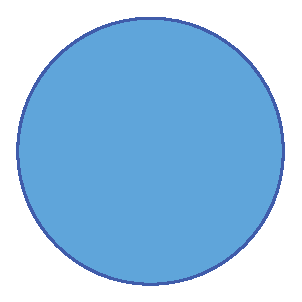
\includegraphics[width=40mm]{image.eps}}
    \end{center}
    \caption{図を並べる例1}
    \label{fig:sample2}
  \end{minipage}
  \begin{minipage}{0.5\hsize}
    \begin{center}
       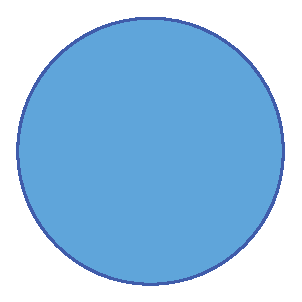
\includegraphics[width=40mm]{image.eps}
    \end{center}
    \caption{図を並べる例2、枠なし}
    \label{fig:sample3}
  \end{minipage}
\end{figure}

\begin{itembox}[l]{{\tt 03.tex}}
\begin{verbatim}
図を二つ横に並べたい場合は、次のように書く(図\ref{fig:sample2}、図\ref{fig:sample3})。

\begin{figure}[htbp]
  \begin{minipage}{0.5\hsize}
    \begin{center}
       \fbox{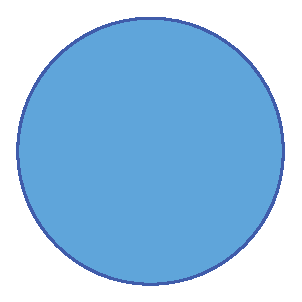
\includegraphics[width=40mm]{image.eps}}
    \end{center}
    \caption{図を並べる例1}
    \label{fig:sample2}
  \end{minipage}
  \begin{minipage}{0.5\hsize}
    \begin{center}
       \fbox{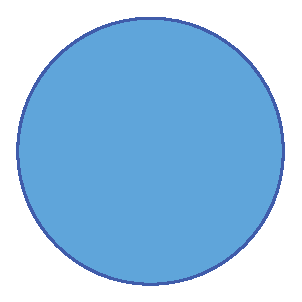
\includegraphics[width=40mm]{image.eps}}
    \end{center}
    \caption{図を並べる例2}
    \label{fig:sample3}
  \end{minipage}
\end{figure}
\end{verbatim}
\end{itembox}


\subsection{表}

表は次のように出力される(表\ref{tb:sample1})。

\begin{table}[htbp]
  \caption{表の例}
  \label{tb:sample1}
  \begin{center}
  \begin{tabular}{l|c|r}
    \hline
    種類	&味&評価\\\hline\hline
    ドラ焼き&甘い&好き\\\hline
    メロンパン&カリもふ&好き\\\hline
    クリームパン&神&すごく好き\\\hline
  \end{tabular}\end{center}
\end{table}

ソースでは次のようになっている。

\begin{itembox}[l]{{\tt 03.tex}}
\begin{verbatim}
表は次のように出力される(表\ref{tb:sample1})。

\begin{table}[htbp]
  \caption{表の例}
  \label{tb:sample1}
  \begin{center}
  \begin{tabular}{l|c|r}
    \hline
    種類	&味&評価\\\hline\hline
    ドラ焼き&甘い&好き\\\hline
    メロンパン&カリもふ&好き\\\hline
    クリームパン&神&すごく好き\\\hline
  \end{tabular}\end{center}
\end{table}
\end{verbatim}
\end{itembox}

{\tt htbp}や \verb|\caption| と \verb|\label| は図と同様。ただし表のタイトルは表の上に書く。

\verb|\begin{tabular}{l|{\tt \textbar}{\tt c}{\tt \textbar}\verb|r}|で横方向のセルを指定する。{\tt c}は中央揃え、{\tt l}は左揃え、{\tt r}は右揃えのセルを作る。{\tt \textbar}は垂直方向の罫線を表す。{\tt c}か{\tt l}か{\tt r}を必要なセルの数だけ並べて、セルの間に罫線が必要なら{\tt \textbar}を入れればよい。

セルの中の文字は、{\tt \&}で区切って並べる。行と行は \verb|\\| で区切る。水平方向の罫線が必要なら、\verb|\hline| を書く。

水平方向や垂直方向のセルの結合もできる。例を示すので、くわしくはぐぐろう。説明がめんどう。\verb|\multirow|、\verb|\multicolumn|、\verb|\cline| を使うとできる。

\begin{table}[htbp]
  \caption{セルを結合した例}
  \label{tb:sample2}
  \begin{center}
  \begin{tabular}{c|c|c}
    \hline
    ほげ&ふー&ばー\\\hline\hline
    \multirow{2}{*}{ほげほげ}&\multicolumn{2}{c}{ふーふー} \\\cline{2-3}
    &ふーふーふー&ばーばーばー\\\hline
  \end{tabular}
  \end{center}
\end{table}

\begin{itembox}[l]{{\tt 03.tex}}
\begin{verbatim}
\begin{table}[htbp]
  \caption{セルを結合した例}
  \label{tb:sample2}
  \begin{center}
  \begin{tabular}{c|c|c}
    \hline
    ほげ&ふー&ばー\\\hline\hline
    \multirow{2}{*}{ほげほげ}&\multicolumn{2}{c}{ふーふー} \\\cline{2-3}
    &ふーふーふー&ばーばーばー\\\hline
  \end{tabular}
  \end{center}
\end{table}
\end{verbatim}
\end{itembox}


\subsection{脚注}

脚注は \verb|\footnote| コマンドを使う。例えばこんな感じ\footnote{ページの下に小さく説明を出せる}。

\begin{itembox}[l]{{\tt 03.tex}}
\begin{verbatim}
例えばこんな感じ\footnote{ページの下に小さく説明を出せる}。
\end{verbatim}
\end{itembox}

\section{その他のコマンド}

ぐぐる\footnote{http://www.google.co.jp/}。

特殊なことは何もしていないテンプレートなので、ぐぐって出たことはだいたいそのまま何でも使える。

あるいは、このファイル自体も\LaTeX で書かれているわけだから、これの{\tt *.tex}を見るのもよいかもしれない。


	% 本文3
\chapter{結論}
\label{chap:conclusion}

この章では、結論らしいことをかく。

\section{まとめ}

\LaTeX の環境さえあればスタンダードな体裁の論文がたぶんだれでも作れる程度のテンプレートにはなっているはず。がんばって卒業しよう。


\section{大事なこと}

箇条書きで列挙する。

\begin{itemize}
 \item ぐぐる。これは単なる\LaTeX だし、\LaTeX はもう枯れた技術だから、調べれば文献はいくらでもある。
 \item 先生を頼る。
 \item 単位をきちんとる。
 \item 卒業する。
\end{itemize}


	% 本文4
\end{verbatim}
\end{itembox}

目次に続いて、論文のメイン、本文を記述する。アブストラクトと同様で、{\tt main.tex}に直接書くか、\verb|\include| コマンドを利用して別に用意したファイルを{\tt include}する。

本文の書き方は、第\ref{chap:latex}章で詳しく説明する。


\subsection{謝辞の出力}

\begin{itembox}[l]{{\tt main.tex}}
\begin{verbatim}
\begin{acknowledgment}
謝辞!!!\\
感謝の言葉を述べる方々はたくさんいらっしゃる...\\
アブストラクトを書いて, 本当の締めで書く.\\
RGの先生方, 仁さん, 大越さん, 陳さん, 柘植さん, 友隆さんを始めとする中澤研究室のファカルティーの方々\\
kgの垣根を超えた大学院の先輩方\\
wataruさん, isokichiさん, drgnmanさん, iphooさんの博士の先輩方,\\
eigenさん,quantan,mokkyさん, ozaさんの修士の先輩方.\\
そしてなにより親のshinsan.\\
兄妹のyuniを始めとする,kg-HAISYSの同期・後輩たち, 中澤研究室の同期後輩たち\\
野中先生のお名前もいれたい, 野中研の研究室メンバーも.\\
そして両親に挨拶をして論文を終わる予定\\

\end{acknowledgment}
	% 謝辞。要独自コマンド、include先参照のこと
\end{verbatim}
\end{itembox}

本文のあとには、謝辞を出力する。\verb|begin{acknowledgment}| から \verb|end{acknowledgment}| の間に書いた文章が、謝辞として独立したページに出力される。アブストラクトや本文と同じで、{\tt main.tex}に直接書いてもよいし、\verb|\include| コマンドを利用して{\tt include}してもよい。


\subsection{参考文献の出力}

\begin{itembox}[l]{{\tt main.tex}}
\begin{verbatim}

\begin{bib}[100]
% BibTeXを使う場合
\bibliography{main}

%\begin{thebibliography}{#1}
%
%  \bibitem{参照用名称}
%    著者名: 
%    \newblock 文献名,
%    \newblock 書誌情報,出版年.
%
% \bibitem{hoge09}
%   ほげ山太郎,ほげ山次郎:
%   \newblock ほげほげ理論のHCI分野への応用,
%   \newblock ほげほげ学会論文誌,Vol.31,No.3,pp.194-201,2009.
% 
% \bibitem{hoge08}
%   Taro Hogeyama, Jiro Hogeyama:
%   \newblock The Theory of Hoge,
%   \newblock {\it The Proceedings of The Hoge Society}, 2008.
%	
%\end{thebibliography}

\end{bib}
	% 参考文献。要独自コマンド、include先参照のこと
\end{verbatim}
\end{itembox}

謝辞に続いて、参考文献を出力する。

参考文献リストは、\verb|\begin{bib}| から \verb|\end{bib}| の間に、\verb|\bibitem| コマンドを使って書く。

BibTeXを使う場合は、以下のようにする。

\begin{itembox}[l]{{\tt 91\_bibliography.tex}}
\begin{verbatim}
\begin{bib}[100]
\bibliography{main}
\end{bib}
\end{verbatim}
\end{itembox}

こうすると、\verb|main.bib|から使用した参考文献のみを抽出して出力してくれる。\verb|main.bib|の中身は以下のようになっていて、気の利いた論文検索サイトであればBibTeXをコピペできるようになっているので簡単に作れるはず。


\begin{itembox}[l]{{\tt 91\_bibliography.tex}}
\begin{verbatim}
@article{hoge09,
    author  = "ほげ山太郎 and ほげ山次郎",
    yomi    = "ほげやまたろう",
    title   = "ほげほげ理論のHCI分野への応用",
    journal = "ほげほげ学会論文誌",
    volume  = "31",
    number  = "3",
    pages   = "194-201",
    year    = "2009",
}
@inproceedings{hoge08,
    author     = "Taro Hogeyama and Jiro Hogeyama",
    title      = "The Theory of Hoge",
    booktitle  = "The Proceedings of The Hoge Society",
    year       = "2008"
}
\end{verbatim}
\end{itembox}


以下は、BibTeXを使わないで手で書く例。

\begin{itembox}[l]{{\tt 91\_bibliography.tex}}
\begin{verbatim}
@article{hoge09,
    author  = "ほげ山太郎 and ほげ山次郎",
    yomi    = "ほげやまたろう",
    title   = "ほげほげ理論のHCI分野への応用",
    journal = "ほげほげ学会論文誌",
    volume  = "31",
    number  = "3",
    pages   = "194-201",
    year    = "2009",
}
@inproceedings{hoge08,
    author     = "Taro Hogeyama and Jiro Hogeyama",
    title      = "The Theory of Hoge",
    booktitle  = "The Proceedings of The Hoge Society",
    year       = "2008"
}
\end{verbatim}
\end{itembox}


英語の文献の場合、慣例的に書誌名をイタリック体にすることが多いらしい。

\begin{itembox}[l]{{\tt 91\_bibliography.tex}}
\begin{verbatim}
\begin{bib}[100]
\begin{thebibliography}{#1}
% \bibitem{参照用名称}
%   著者名:
%   \newblock 文献名,
%   \newblock 書誌情報,出版年.

\bibitem{hoge09}
  ほげ山太郎,ほげ山次郎:
  \newblock ほげほげ理論のHCI分野への応用,
  \newblock ほげほげ学会論文誌,Vol.31,No.3,pp.194-201,2009.

\bibitem{hoge08}
  Taro Hogeyama, Jiro Hogeyama:
  \newblock The Theory of Hoge,
  \newblock {\it The Proceedings of The Hoge Society}, 2008.
\end{thebibliography}
\end{bib}
\end{verbatim}
\end{itembox}

\verb|\bibitem| コマンド中、参照用名称は、本文から参考文献を参照するときに使うので、忘れずに書いておく。参照文献を本文中に参照するときには、\verb|\cite{参照用名称}| のように書けばよい。例えば、この文の末尾には \verb|\cite{hoge09}| と書いてあるので、自動で対応する番号が振られる\cite{hoge09}\cite{hoge08}。

参考文献リストの番号付けと、本文で参照したときの番号の挿入は、全部が自動で行われる。ただしこれも、第\ref{sec:toc}節で説明した目次の出力と同じで、一時ファイルを生成してからの挿入なので、正しく出力するには最低でも二回のコンパイルが必要。BibTeXを使用する場合は、\verb|platex|コマンドのあと\verb|pbibtex|コマンドを実行し、さらに2回\verb|platex|コマンドを実行するといいらしい。



\subsection{付録の出力}

\begin{itembox}[l]{{\tt main.tex}}
\begin{verbatim}
\appendix
\chapter{付録の例}

付録を無理矢理出力させるため、てきとうなことを書く。

\section{ほげ}

コマンドは本文と一緒。

\subsection{ふー}

本文と一緒。

\section{ほげほげ}

本文と一緒。

\subsection{ふーふー}

本文と一緒。
		% 付録
\end{verbatim}
\end{itembox}

必要であれば、論文の最後には付録を出力する。

\verb|\appendix| コマンド以降に書いたものは、すべて付録として扱われる。付録部分の書き方は通常の本文とまったく同じで、\verb|\appendix| コマンド以降に書くだけで勝手に付録用の体裁で出力される。
  % 本文2
%\chapter{\LaTeX の書き方}
\label{chap:latex}

この章では、よく使う\LaTeX のコマンドを説明する。足りない部分はぐぐればだいたいわかると思う。最初に書いておくと、数式を書く方法は、ぼく自身使わなかったので書いていない。ぼくのいた研究室でごりごり数式をたくさん書く必要のあるひとは、研究の種類からするとあまり居ない気がする。

\section{主なコマンド}

\subsection{章と節}

文書構造を明確にする大事なもの。目次はこれらのコマンドをもとに作られる。例えば、この第\ref{chap:latex}章の冒頭部分はこのようなソースで書かれている。

\begin{itembox}[l]{{\tt 03.tex}}
\begin{verbatim}
\chapter{\LaTeX の書き方}
\label{chap:latex}

この章では、よく使う\LaTeX のコマンドを説明する。(略)

\section{主なコマンド}

\subsection{章と節}

文書構造を明確にする大事なもの。目次はこれらのコマンドをもとに作られる。例えば、この第\ref{chap:latex}章の冒頭部分はこのようなソースで書かれている。
\end{verbatim}
\end{itembox}

章は \verb|\chapter{見出し}|、節は \verb|\section{見出し}|、小節は \verb|\subsection{見出し}|、小々節は \verb|\subsubsection{見出し}| を使う。表\ref{tb:chap}に一覧する。

\begin{table}[htbp]
  \caption{章と節のコマンド}
  \label{tb:chap}
  \begin{center}\begin{tabular}{c|c}
    \hline
    コマンド&用途\\\hline\hline
    \verb|\chapter{見出し}|&章\\\hline
    \verb|\section{見出し}|&節\\\hline
    \verb|\subsection{見出し}|&小節\\\hline
    \verb|\subsubsection{見出し}|&小々節\\\hline
    \end{tabular}\end{center}
\end{table}

\subsubsection{小々節見出しサンプルその1}

小々節は上のように \verb|\subsubsection{タイトル}| で書けるけれど、あまり文書の階層構造が深いことは望ましくないので、多用しなければならないようなら文書構造を見直したほうがよいと思う。

\subsubsection{小々節見出しサンプルその2}

小々節は、章や節、小節のように {\tt N.N.N} といった番号ではなくて、括弧付きの番号で出力される。かつ、目次には出力されない。

\subsection{図}

図は次のように出力される(図\ref{fig:sample1})。

\begin{figure}[htbp]
    \begin{center}
       \fbox{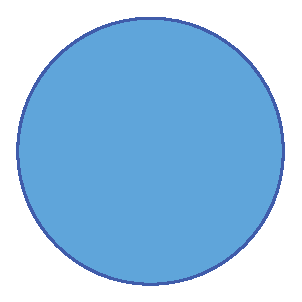
\includegraphics[width=50mm]{image.eps}}
    \end{center}
    \caption{図の例}
    \label{fig:sample1}
\end{figure}

ソースでは次のように記述している。

\begin{itembox}[l]{{\tt 03.tex}}
\begin{verbatim}
図は次のように出力される(図\ref{fig:sample1})。

\begin{figure}[htbp]
    \begin{center}
       \fbox{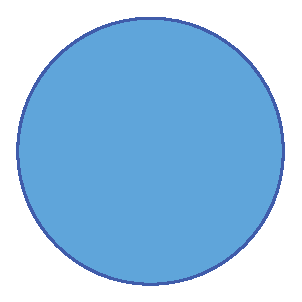
\includegraphics[width=40mm]{image.eps}}
    \end{center}
    \caption{図の例}
    \label{fig:sample1}
\end{figure}
\end{verbatim}
\end{itembox}

\verb|\begin{figure}[htbp]|  の{\tt htbp}は、表示位置の優先順位の設定。基本的に\LaTeX では、図の挿入位置は強制的には指定できない。いくつか候補を指定しておくと、候補のなかの優先度の高い順に、図を入れられるスペースがあるかどうかを調べて、入れられればそこに、入れられなければ次の候補のスペースを調べる、という処理が行われる。{\tt h}はこのコマンドを書いたその場所に、{\tt t}はページの一番上に、{\tt b}はページの一番下に、{\tt p}は画像だけ別ページに、それぞれ配置する。基本的には{\tt htbp}のように全部書いておけば問題ない。

\verb|\includegraphics| コマンドで、図のサイズと挿入するファイルを指定する。上の例ではサイズは {\tt width=50mm} として幅を指定したけれど、ここは他にも {\tt height=30mm} として高さを指定してもよいし、{\tt scale=0.5} として拡大率を指定してもよい。画像は最近の \LaTeX 環境であれば{\tt *.eps}以外でも使える。ただし、{\tt bb} (Bounding Box) として画像の大きさを指定する必要があることも多い。
以下はJPEG画像を使用する例。

\begin{itembox}[l]{{\tt 03.tex}}
\begin{verbatim}
\begin{figure}[htbp]
    \begin{center}
       \fbox{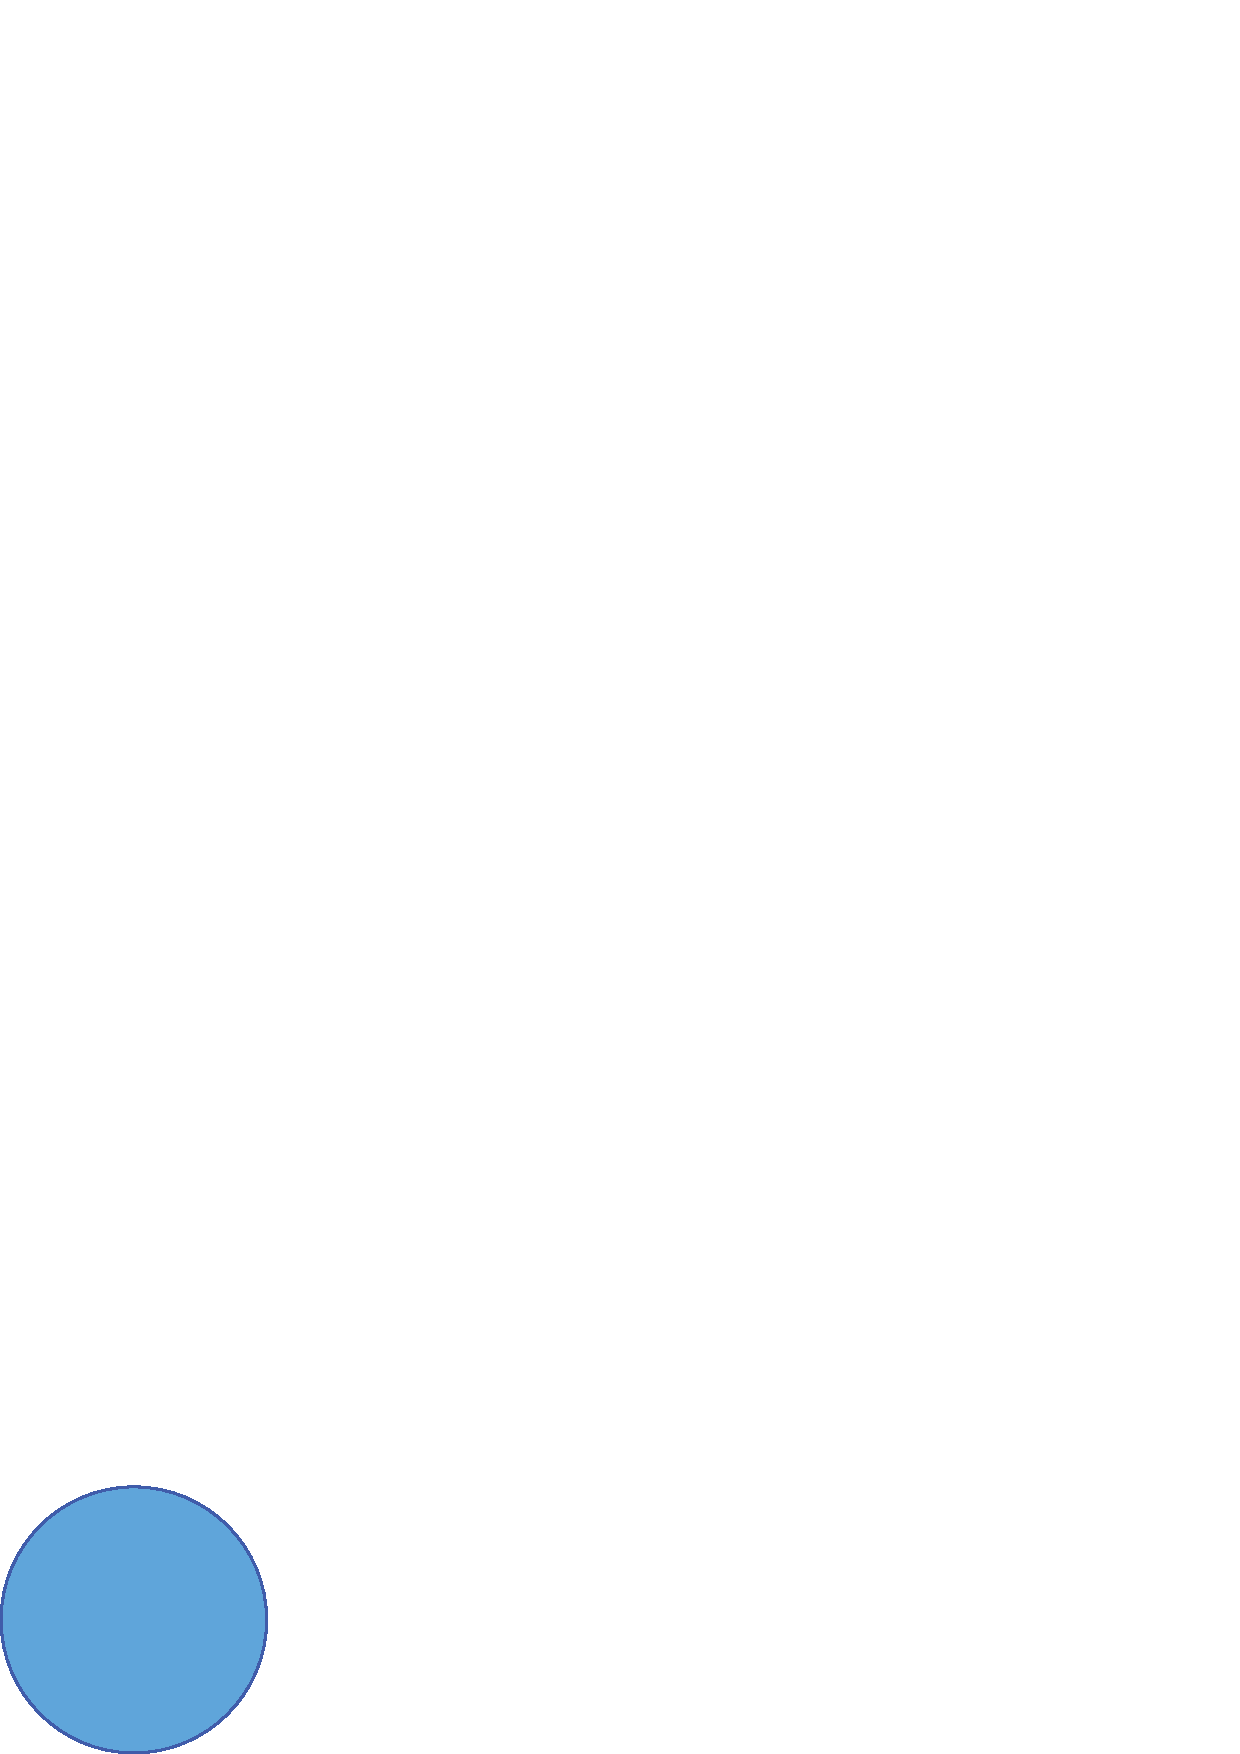
\includegraphics[width=40mm,bb=0 0 640 480]{image.jpg}}
    \end{center}
    \caption{図の例}
    \label{fig:sample1}
\end{figure}
\end{verbatim}
\end{itembox}

bbの指定は、上記のように{\tt *.tex} ファイルの中で指定してもいいが、
{\tt *.bb}ファイルを作っておく方法もある。
ターミナルで{\tt ebb}コマンドを使用すると{\tt *.bb}ファイルを簡単に作れる。


\begin{itembox}[l]{ebbコマンドの例}
\begin{verbatim}
% ebb image.jpg
\end{verbatim}
\end{itembox}


\verb|\includegraphics| を \verb|\fbox| に入れると、画像に枠を付けられる。

\verb|\caption| コマンドで図の見出しを指定できる。図の見出しは、図の下に表記するので注意。ここで指定した見出しが、図の目次に表示される。

\verb|\label| コマンドでは図の参照用ラベルを設定できる。本文中、\verb|\ref| コマンドで参照用ラベルを指定すると、対応した図の番号が自動的に挿入される。これも目次や参考文献と同様、最低二回のコンパイルが必要なので注意。

図を二つ横に並べたい場合は、次のように書く(図\ref{fig:sample2}、図\ref{fig:sample3})。

\begin{figure}[htbp]
  \begin{minipage}{0.5\hsize}
    \begin{center}
       \fbox{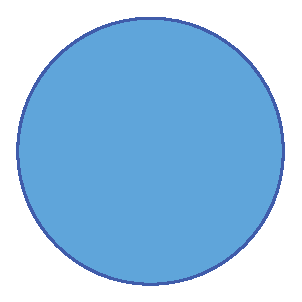
\includegraphics[width=40mm]{image.eps}}
    \end{center}
    \caption{図を並べる例1}
    \label{fig:sample2}
  \end{minipage}
  \begin{minipage}{0.5\hsize}
    \begin{center}
       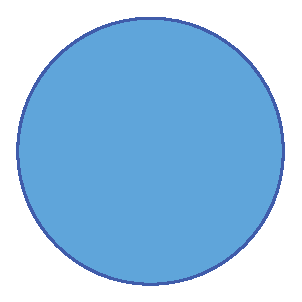
\includegraphics[width=40mm]{image.eps}
    \end{center}
    \caption{図を並べる例2、枠なし}
    \label{fig:sample3}
  \end{minipage}
\end{figure}

\begin{itembox}[l]{{\tt 03.tex}}
\begin{verbatim}
図を二つ横に並べたい場合は、次のように書く(図\ref{fig:sample2}、図\ref{fig:sample3})。

\begin{figure}[htbp]
  \begin{minipage}{0.5\hsize}
    \begin{center}
       \fbox{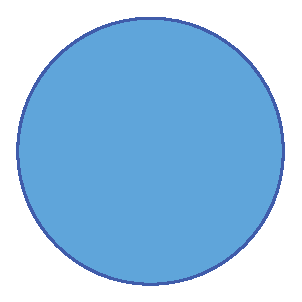
\includegraphics[width=40mm]{image.eps}}
    \end{center}
    \caption{図を並べる例1}
    \label{fig:sample2}
  \end{minipage}
  \begin{minipage}{0.5\hsize}
    \begin{center}
       \fbox{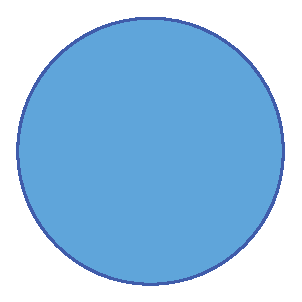
\includegraphics[width=40mm]{image.eps}}
    \end{center}
    \caption{図を並べる例2}
    \label{fig:sample3}
  \end{minipage}
\end{figure}
\end{verbatim}
\end{itembox}


\subsection{表}

表は次のように出力される(表\ref{tb:sample1})。

\begin{table}[htbp]
  \caption{表の例}
  \label{tb:sample1}
  \begin{center}
  \begin{tabular}{l|c|r}
    \hline
    種類	&味&評価\\\hline\hline
    ドラ焼き&甘い&好き\\\hline
    メロンパン&カリもふ&好き\\\hline
    クリームパン&神&すごく好き\\\hline
  \end{tabular}\end{center}
\end{table}

ソースでは次のようになっている。

\begin{itembox}[l]{{\tt 03.tex}}
\begin{verbatim}
表は次のように出力される(表\ref{tb:sample1})。

\begin{table}[htbp]
  \caption{表の例}
  \label{tb:sample1}
  \begin{center}
  \begin{tabular}{l|c|r}
    \hline
    種類	&味&評価\\\hline\hline
    ドラ焼き&甘い&好き\\\hline
    メロンパン&カリもふ&好き\\\hline
    クリームパン&神&すごく好き\\\hline
  \end{tabular}\end{center}
\end{table}
\end{verbatim}
\end{itembox}

{\tt htbp}や \verb|\caption| と \verb|\label| は図と同様。ただし表のタイトルは表の上に書く。

\verb|\begin{tabular}{l|{\tt \textbar}{\tt c}{\tt \textbar}\verb|r}|で横方向のセルを指定する。{\tt c}は中央揃え、{\tt l}は左揃え、{\tt r}は右揃えのセルを作る。{\tt \textbar}は垂直方向の罫線を表す。{\tt c}か{\tt l}か{\tt r}を必要なセルの数だけ並べて、セルの間に罫線が必要なら{\tt \textbar}を入れればよい。

セルの中の文字は、{\tt \&}で区切って並べる。行と行は \verb|\\| で区切る。水平方向の罫線が必要なら、\verb|\hline| を書く。

水平方向や垂直方向のセルの結合もできる。例を示すので、くわしくはぐぐろう。説明がめんどう。\verb|\multirow|、\verb|\multicolumn|、\verb|\cline| を使うとできる。

\begin{table}[htbp]
  \caption{セルを結合した例}
  \label{tb:sample2}
  \begin{center}
  \begin{tabular}{c|c|c}
    \hline
    ほげ&ふー&ばー\\\hline\hline
    \multirow{2}{*}{ほげほげ}&\multicolumn{2}{c}{ふーふー} \\\cline{2-3}
    &ふーふーふー&ばーばーばー\\\hline
  \end{tabular}
  \end{center}
\end{table}

\begin{itembox}[l]{{\tt 03.tex}}
\begin{verbatim}
\begin{table}[htbp]
  \caption{セルを結合した例}
  \label{tb:sample2}
  \begin{center}
  \begin{tabular}{c|c|c}
    \hline
    ほげ&ふー&ばー\\\hline\hline
    \multirow{2}{*}{ほげほげ}&\multicolumn{2}{c}{ふーふー} \\\cline{2-3}
    &ふーふーふー&ばーばーばー\\\hline
  \end{tabular}
  \end{center}
\end{table}
\end{verbatim}
\end{itembox}


\subsection{脚注}

脚注は \verb|\footnote| コマンドを使う。例えばこんな感じ\footnote{ページの下に小さく説明を出せる}。

\begin{itembox}[l]{{\tt 03.tex}}
\begin{verbatim}
例えばこんな感じ\footnote{ページの下に小さく説明を出せる}。
\end{verbatim}
\end{itembox}

\section{その他のコマンド}

ぐぐる\footnote{http://www.google.co.jp/}。

特殊なことは何もしていないテンプレートなので、ぐぐって出たことはだいたいそのまま何でも使える。

あるいは、このファイル自体も\LaTeX で書かれているわけだから、これの{\tt *.tex}を見るのもよいかもしれない。


  % 本文3
%\chapter{結論}
\label{chap:conclusion}

この章では、結論らしいことをかく。

\section{まとめ}

\LaTeX の環境さえあればスタンダードな体裁の論文がたぶんだれでも作れる程度のテンプレートにはなっているはず。がんばって卒業しよう。


\section{大事なこと}

箇条書きで列挙する。

\begin{itemize}
 \item ぐぐる。これは単なる\LaTeX だし、\LaTeX はもう枯れた技術だから、調べれば文献はいくらでもある。
 \item 先生を頼る。
 \item 単位をきちんとる。
 \item 卒業する。
\end{itemize}


  % 本文4
\chapter{関連研究}
\label{chap:smile}

本章では, はじめに人の表情についての関連研究ついてまとめる.
ついで, 情報学の分野における表情, 特に笑顔に関する先行研究の例を取り上げる.
最後に, 本研究において取り扱う笑顔について定義する.

\section{人と表情に関する研究}
本セクションでは, 人の表情についての関連研究および表情と人間関係の関連性の2つについてまとめる.
\subsection{人の表情について}
Ekmanは感情を表す普遍的な基本表情があるという理論を提唱した.
その表情は7つに分類され, 怒り,嫌悪,恐怖,驚き,悲しみ,幸福に中立な表情を加えたものである.\cite{ekman}
\begin{figure}[htbp]
    \begin{center}
       \fbox{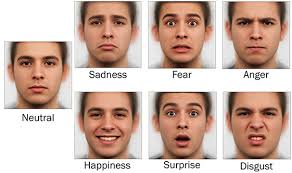
\includegraphics[width=120mm,bb=0 0 292 173]{universal_facial_expressipn.jpeg}}
    \end{center}
    \caption{普遍7表情}
    \label{fig:universal_facial_expression}
\end{figure}
佐藤らが日本人に対して, Ekmanの基本表情が適用されるのかを実験した際には,
部分的にしか日本人には適応されないことがわかったが, 驚きと幸福に関する基本表情は日本人にも
適合することが証明されている.\cite{JapaneseFacialExpression}
\begin{figure}[htbp]
    \begin{center}
       \fbox{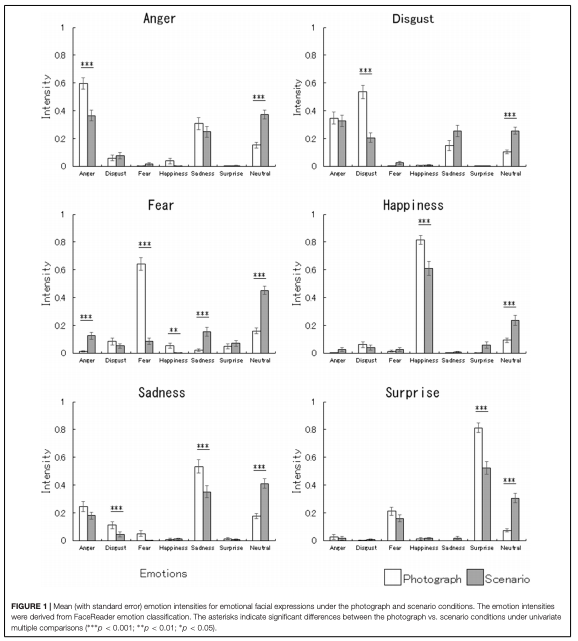
\includegraphics[width=80mm,bb=0 0 578 641]{emotion_graph.jpg}}
    \end{center}
    \caption{日本人の表情判断グラフ}
    \label{fig:JapaneseFacialExpression}
\end{figure}

\subsection{人間関係と表情について}
顔には年齢, 性別, 人種などの生物学的属性に加え, 口の動きからの発話情報, その人物の人となり, 感情, 意図, 関心などを読み取ることが可能である.\cite{role_facialexpression_in_communication}
人はコミュニケーションをとる際に, 会話の内容などの言語コミュニケーションに加え, 表情などの非言語コミュニケーションが行われる.
非言語コミュニケーションとは, 言葉を使わないコミュニケーションのことを指し, メラビアンによればコミュニケーションにおいて,
非言語コミュニケーションは印象情報の93\% を占める.\cite {rule_of_Mehrabian}
ゆえに, コミュニケーションにおいて会話内容よりも, 人の見た目や表情に意識がむく.
表情, 特に笑顔はコミュニケーションをとる際に重要な役割を担っている.



\section{情報技術と笑顔に関する研究}
近年, 情報処理技術を用いて人の表情分析の研究が進められている.
SONYが開発し, デジタルカメラ Cyber shotに組み込まれているスマイルシャッターなどは笑顔検出技術を用いて,
システム搭載されている例である.実用化が進んでいるが, より笑顔を検出する精度や速さが求められている.
\begin{figure}[htbp]
    \begin{center}
       \fbox{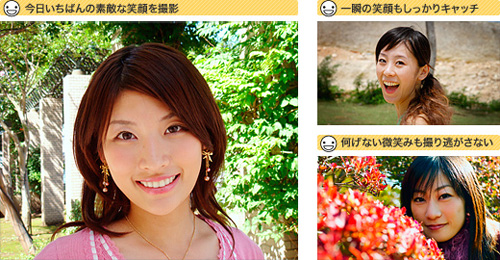
\includegraphics[width=100mm,bb=0 0 500 260]{sony_smile_shutter.jpg}}
    \end{center}
    \caption{SONYスマイルシャッター}
    \label{fig:sony_smile_shutter}
\end{figure}

Eduardらは口角をベースとした笑顔検出器を作成し, 既存の検知方法よりも速く笑顔の検出を可能にする手法の提案をしている.\cite{EduardRoyce}
人の笑顔を顔のパーツ, 特に目や口元, 頬の動きを判断材料として, 画像処理技術および機械学習を用いて自動的に笑顔を検出するような研究が数多く行われている.
他にも表情に現れる感情と, 実際に抱いている感情との違いを検出するような研究も行われている.
実際に人同士でも相手の内面状態を知ることは非常に難しい. 不快感を抱いていたとしても 相手に悟られないように笑顔を作るなど表情と感情が一致しないケースも数多くある.
I Gede Aris Gunadiらは,画像から機械学習を用いた作り笑顔を検出する研究\cite{IGedeArisGunadi}, Neeleshらは動画を用いて作り笑顔の検出\cite{NeeleshBhakt}を行うなど人の表情と内面状態との乖離を解消するような研究も進んでいる.

\section{本研究において取り扱う笑顔}
本研究では, 笑顔を内面の感情ではなく表情のみを取り扱う. %この理由を述べる(修正)
笑顔の作り方を分析し, 表出表現による自分の表情と相手の表情への嗜好判断を行う.
笑顔の分析オープンソースであるOpenFaceの中に含まれる, Facial Action Unitを用いて行う.
OpenFaceとはTadasらCambridge University, MultiCamp Labが作成した表情分析を行うためのツールである.
Facial Action Unit(以下FAUとする)は,Paul Ekman,Wallace Friesenらによって1978年に開発された分析ツールかつ表情理論に基づいたFacial Action Coding System
を使って,客観的に顔の動きをデータとして取得することのできる基本動作を定義したものである.
\begin{figure}[htbp]
    \begin{center}
       \fbox{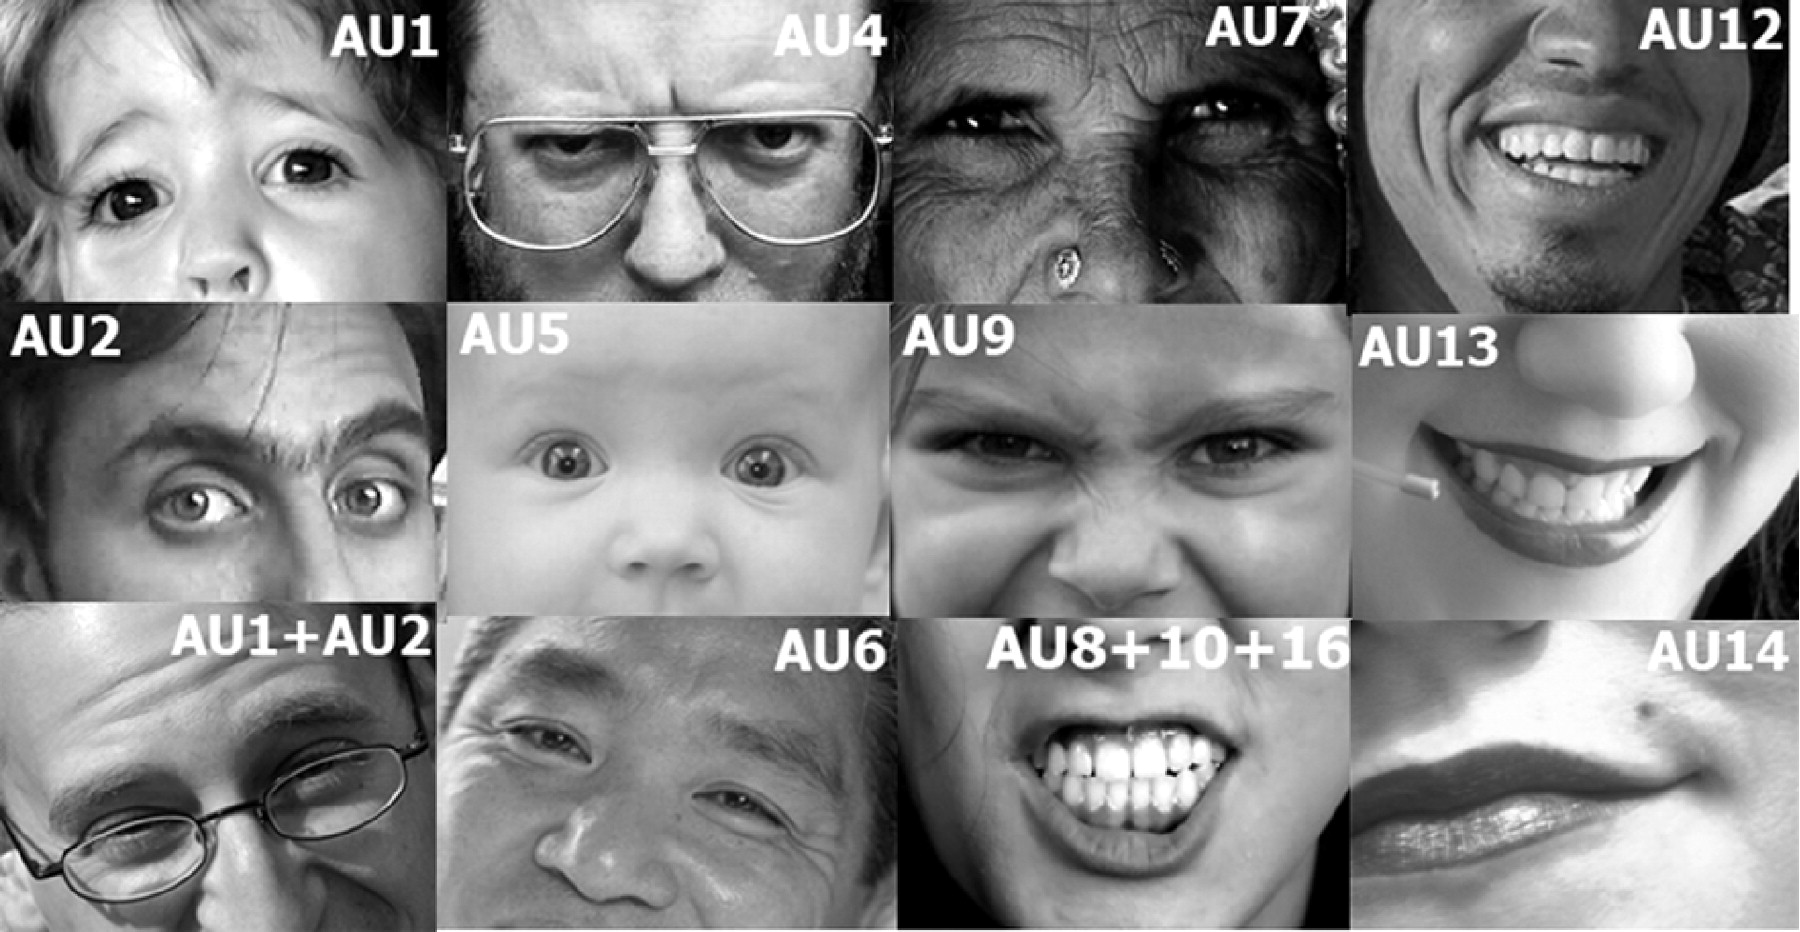
\includegraphics[width=120mm,bb=0 0 1800 932]{faus.jpg}}
    \end{center}
    \caption{Facial Action Unit}
    \label{fig:faus}
    \end{figure}

    \begin{figure}[htbp]
        \begin{center}
           \fbox{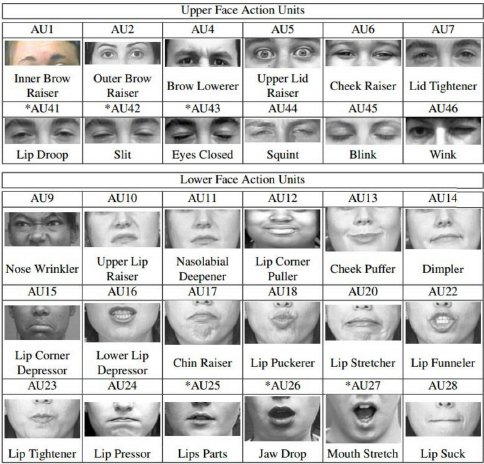
\includegraphics[width=120mm,bb=0 0 484 464]{faus2.jpg}}
        \end{center}
        \caption{Facial Action Unit 種類}
        \label{fig:faus2}
        \end{figure}
  FAUにおいて,笑顔のunit番号は6(眼窩部眼輪筋),7(眼瞼部眼輪筋),12(大頬骨筋),25(翼突筋+顎二腹筋)である.
  この4つのUnitを使用して笑顔の分析を本研究では行う.
\section{まとめ}
本章では, 現在行われている人の表情, 特に笑顔についての先行研究について整理した.
ついで, 本研究で扱うFacial Action Unit を用いて判断する笑顔について定義した.
次章では本研究において使用する, Delta Smile Facial Survey Analyzer のシステムの概要および特徴について述べる.
  % 先行研究まとめ
\chapter{DSFSA(Delta Smile Facial Survey Analyzer)システム}
\label{chap:aboutDSFSA}

本章では, 本研究の目的である笑顔からお互いを分析し, 人と人との繋がり作成を助長するシステムを作成するための,
データ収集およびデータ分析をするためのツールDelta Smile Facial Survey Analyzer(以下DSFSA)について述べる.
初めにシステムの大まかな流れを述べた後, 本システムの特徴および使用方法について述べる.


\section{DSFSAシステムの概要}
本システムは表情分析をするためのデータを収集するためのツールである.
ユーザーの顔を検出し,トラッキングをする.
ユーザーが中立の表情から笑顔になったタイミングでトラッキングを終了し,
各フレームごとに画像処理をして表情の分析を行い動画としてデータベースへ保存する.
Open FaceのFacial Action Unit を使用して特徴量を算出した後,
データベースの中にある決まったフォーマットの笑顔の作り方ので動画を5種類選択し,ユーザーに表示する.
その際には, 顔の特徴点のみを描画した動画を表示することで表情の動き以外のバイアスを軽減する.
選択した動画を2つずつ表示し, ユーザーに好みを選んでもらうことで動画データに順位づけを行う.
ユーザーの表情データ, 選ばれたデータベース内の動画を分析した表情データ, および順位づけデータを使用して,
ユーザーの表情と, ユーザーの嗜好表情との関連性を分析する.

\section{DSFSAの特徴}
本システムの特徴は, 中立と笑顔の表情を部分的に切り取った断片的な画像データではなく,
動画の形を採用することで表情の遷移を時系列データで, 笑顔の作り方を記録し,分析することが可能である.
SONYが開発したスマイルシャッタ-のように笑顔になったタイミングをキャプチャーするシステムなど[sonyのやつ]
笑顔のタイミングのみにフォーカスをあてた研究やサービス,笑顔のタイミングのみを切り取って表情分析をする研究は盛んに行われているが,
動画など時系列データを使用した表情分析系の研究はまだ少ない.
Bruce \& Youngらは表情表出の時間的特性が感情の認知に影響を及ぼす結果を得ており,
感情の認識においては動画像解析による動的な特徴を抽出することが望ましいと述べている.\cite{KOkata} \cite{yukiTakahasshi}
本システムにおいては, 中立表情から笑顔になるまでの表情の遷移を記録し,
顔のパーツの動き, 筋肉の動きを数値化することが可能である.
数値化可能な値は, 顔のパーツの位置, 動きがあるかないかの2極値, そして動きの強度である.

\section{DSFSAの使用方法}
2つのモードを使いわけて, 笑顔の作り方を記録した動画データを作成することおよび顔パーツの動きを
数値化することが可能である.
また, 中立の表情から笑顔になるタイミングを記録した動画データのことを以下では笑顔動画データとする.
\subsection{動画から笑顔動画データ作成および数値化}
人が映った既存の動画データから, 笑顔動画データを作成することが可能である.
ユーザーに表示するための笑顔動画データを作成, 収集するために使用するモードである.
\subsection{ユーザー表情の笑顔動画データ作成および数値化}
実際にユーザーの表情の動きをトラッキングして, 笑顔動画データを作成することが可能である.
表情と嗜好の関係性をするためのデータを収集およびユーザーの笑顔動画データをデータベースに
保存するためのモードである.

\section{まとめ}
本章では, 笑顔動画データ作成および収集, 数値化を行う本システムの概要について述べた.
ついで, 本システムの特徴および使用方法について説明をした.
次章では, Delta Smile Facial Survey Analyzer システムの設計について述べる.
  % システムについて
\chapter{設計}
\label{chap:function}

この章ではDESFAの設計について述べる.

\section{本システムの設計概要}
\section{顔検出モジュール}
\section{笑顔検出モジュール}
\section{画像処理モジュール}
\section{動画作成モジュール}
\section{表示データ作成モジュール}
\section{ランキングデータ取得モジュール}
\section{データ保存モジュール}
\section{笑顔トリミングモジュール}
\section{csvモジュール}
\section{データプロットモジュール}
\section{まとめ}
  % 機能要件
\chapter{実装}
\label{chap:developing}
本章では, Delta Smile Facial Survey Analyzer の実装部分について説明する.
まずユーザーインターフェースの実装について説明し, システム全体の画面遷移の流れを最初に示す.
次にデータ収集機能の各モジュールの実装について整理し, データ分析機能の各モジュールの実装について
説明し,まとめる.

\section{ユーザーインターフェースの実装}
本システムではおよそ3分程度で一連のデータ収集機能のシステム処理を行う.
開発言語はpythonを使用し, バージョンは3.6.1 を使用した.
実行コマンドは以下のように行う. mode\_num は0を引数に指定するとユーザーからのデータを収集し,
1を指定すると既存の動画に対して処理を行いデータ形成を行うことできる.

\begin{itemize}
\item 実行コマンド
\begin{lstlisting}
$ python dsfsa.py mode_num
\end{lstlisting}
%複数の時は以下のように
%\item 実行コマンド
%\begin{lstlisting}
%$ python dsfsa.py mode_num
%\end{lstlisting}
\end{itemize}

ユーザーに見せるシーンとして全部で8種類のシーンが存在する.
各シーンは全てオープンソースのOpenCVを使用して, ディスプレイeizo sx2761wに表示をしている.
それぞれの表示内容, 役割について以下に述べる.

\subsection{ユーザーインターフェースシーン1}
図\ref{fig:seen1}のシーン1はシステムを起動した最初のシーンである.
実験の際に, 個人情報である表情のデータを使うため, ユーザーの同意が必要である.
パソコンのReturnキーを一回入力することで実験, データ提供への同意を得るように実装を行った.

\subsection{ユーザーインターフェースシーン2}
図\ref{fig:seen2}のシーン2はユーザーの基本情報を収集するためのシーンである.
基本情報として, 性別と年齢を何十歳の形で入力をする.
入力したデータは.txtファイルとしてユーザーごとのフォルダーに保存するようにした.

\subsection{ユーザーインターフェースシーン3}
図\ref{fig:seen2}のシーン2にて,基本情報を入力したのちに, 図\ref{fig:seen3}のシーン3へ自動で遷移する.
このシーンでは実際にユーザーの映像がwebカメラ,Logicool C920r の映像が映し出される.
遷移と同時にカメラに映る一番大きな顔をユーザーの顔として認識をしトラッキングを行っている.

\subsection{ユーザーインターフェースシーン4}
図\ref{fig:seen4}のシーン4では, 図\ref{fig:seen3}のシーン3にて, 笑顔が検出された場合にはユーザーの笑顔が検出されていることを知らせる
小さいウィンドウが表示され, 検出した口元に緑色の長方形が描画されるようになっている.

\subsection{ユーザーインターフェースシーン5}
図\ref{fig:seen4}のシーン4にて, 笑顔が一定フレーム以上検出された後, 図\ref{fig:seen5} のシーン5へ移動する.
シーン5が表示されている間にフレーム分析処理, 動画作成処理, データ選択処理が行われており,
およそ20秒ほど処理を待機する時間が発生する.

\subsection{ユーザーインターフェースシーン6}
図\ref{fig:seen6}のシーン6はユーザーから入力を受け付けるシーンである.
点描画によって映し出されている笑顔動画データに対して順位づけを行う.
計5つ, 4回のキーボード入力を行い, 各笑顔動画データに対して順位づけデータを与える.

\subsection{ユーザーインターフェースシーン7}
図\ref{fig:seen7}のシーン7は結果表示画面であり, ユーザーの笑顔動画データを左側, 右側にユーザーが1番高く
順位づけした笑顔動画データを並列で表示する.

\subsection{ユーザーインターフェースシーン8}
図\ref{fig:seen8}のシーン8はシステム終了前のシーンである.
笑顔動画データベースおよび収集した笑顔動画データの中に含まれる全ての笑顔フレームを表示する.

\begin{figure}[htbp]
    \begin{center}
       \fbox{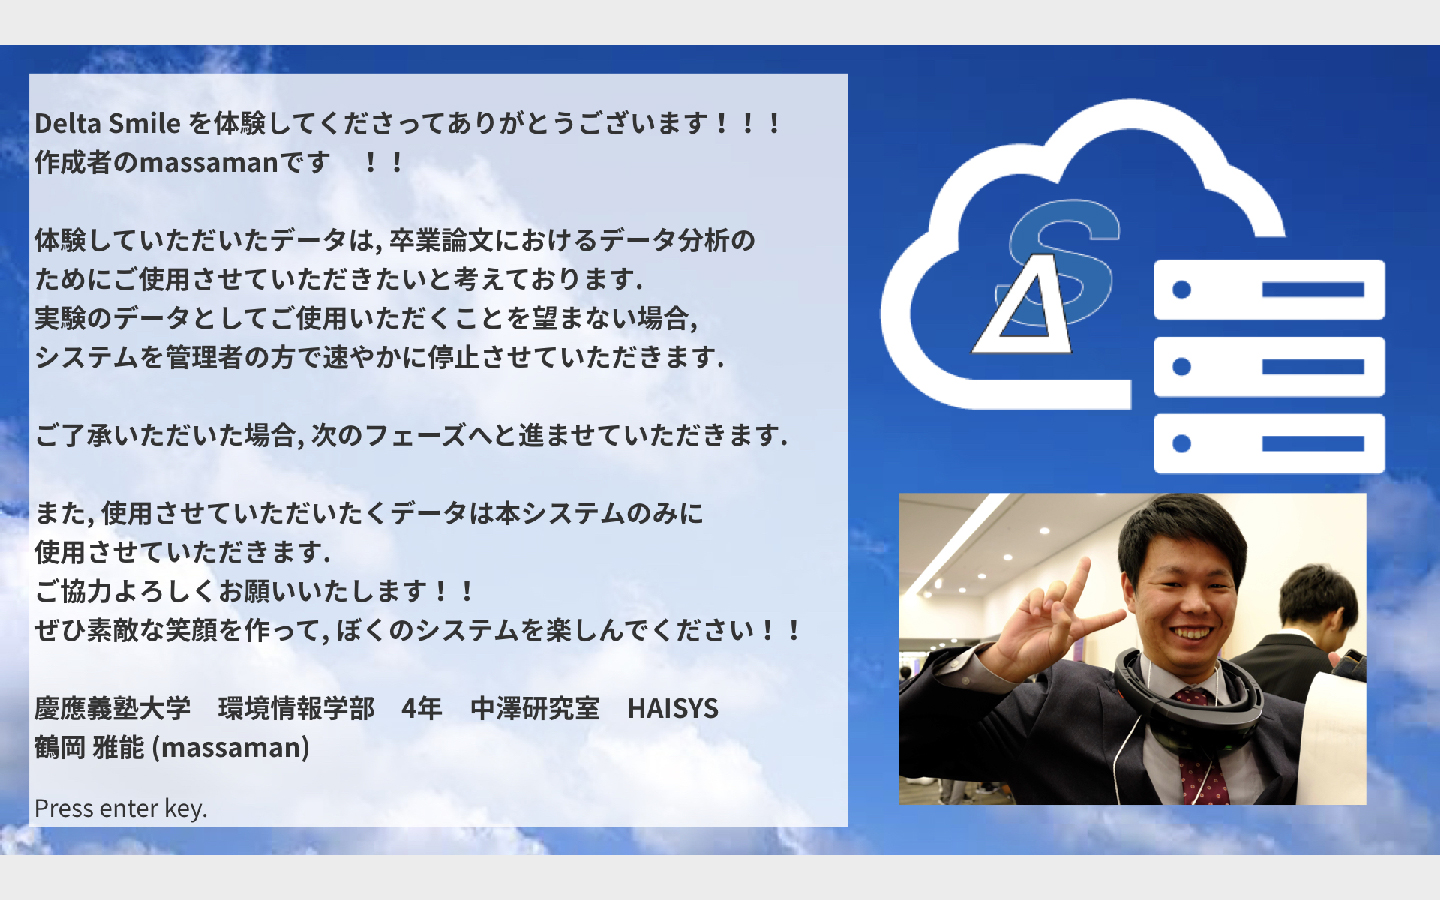
\includegraphics[width=140mm,bb=0 0 1440 900]{seen1.jpg}}
    \end{center}
    \caption{ユーザーインターフェースシーン1}
    \label{fig:seen1}
\end{figure}

\begin{figure}[htbp]
    \begin{center}
       \fbox{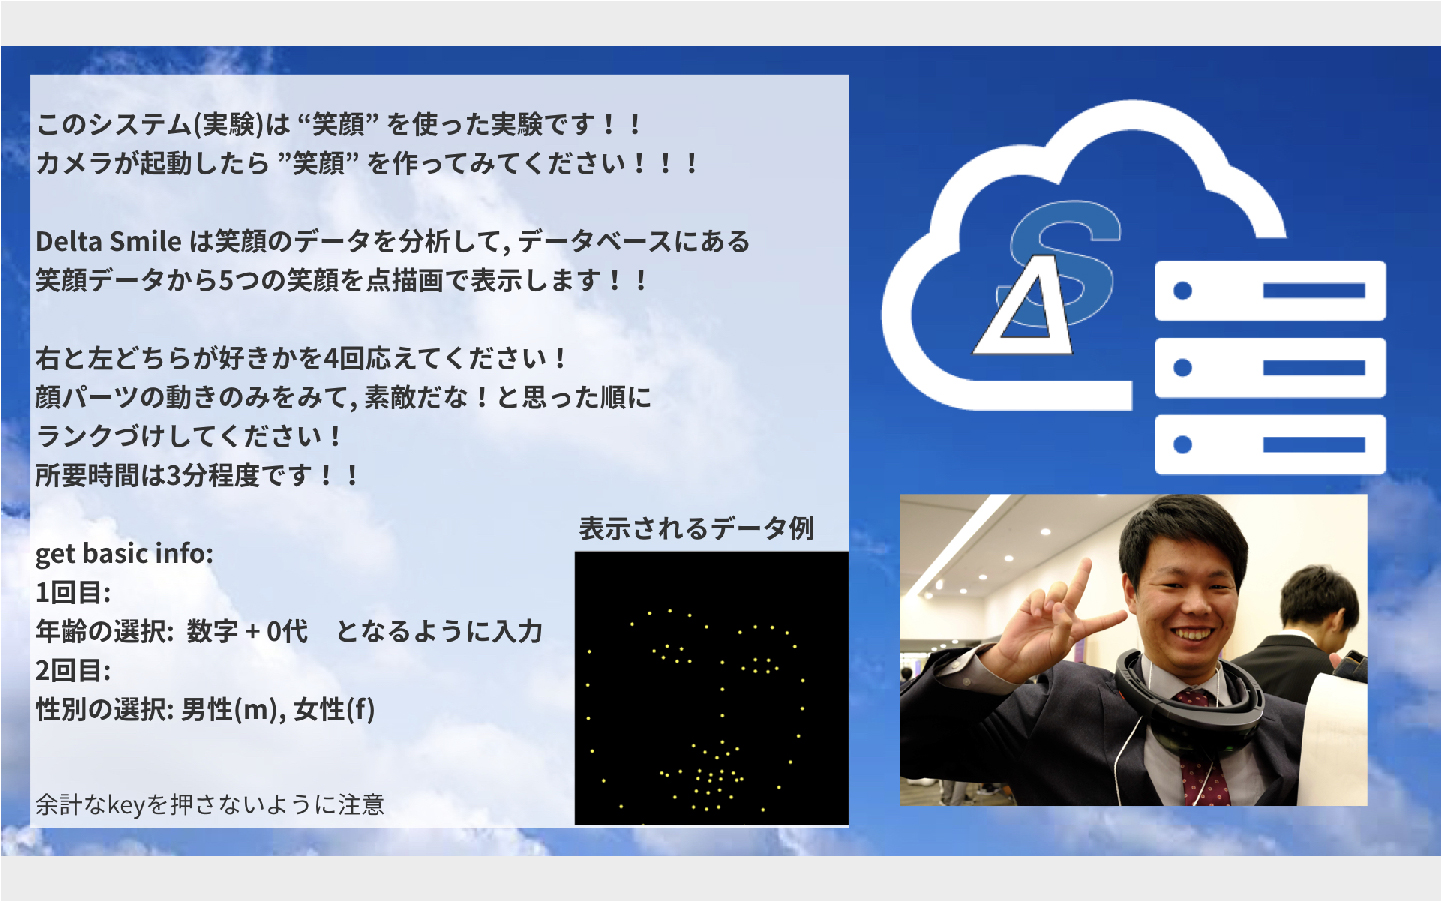
\includegraphics[width=140mm,bb=0 0 1440 900]{seen2.jpg}}
    \end{center}
    \caption{ユーザーインターフェースシーン2}
    \label{fig:seen2}
\end{figure}

\begin{figure}[htbp]
    \begin{center}
       \fbox{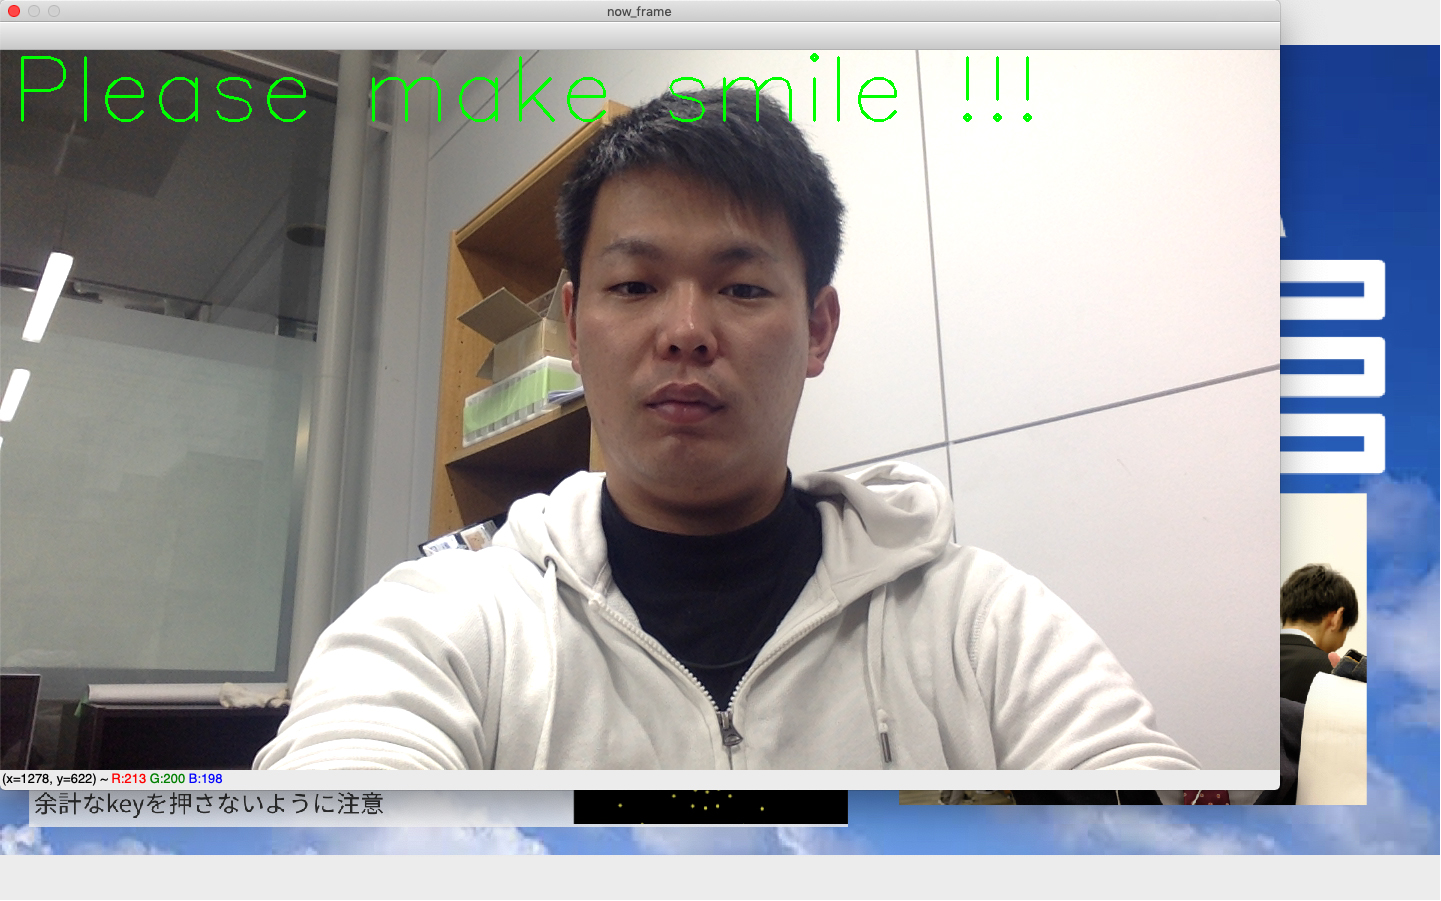
\includegraphics[width=140mm,bb=0 0 1440 900]{seen3.jpg}}
    \end{center}
    \caption{ユーザーインターフェースシーン3}
    \label{fig:seen3}
\end{figure}

\begin{figure}[htbp]
    \begin{center}
       \fbox{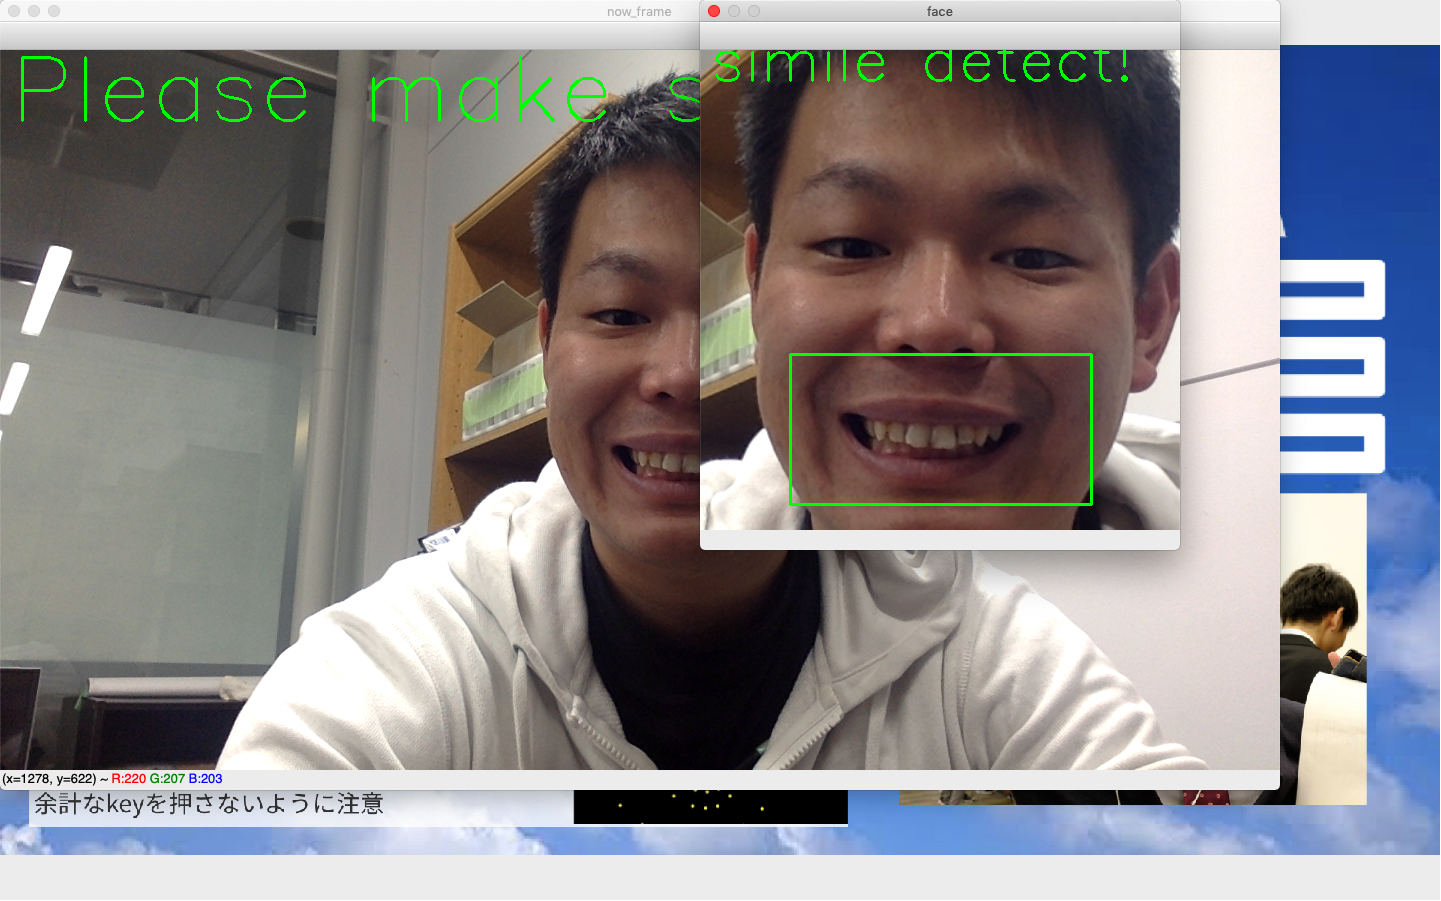
\includegraphics[width=140mm,bb=0 0 1440 900]{seen4.jpg}}
    \end{center}
    \caption{ユーザーインターフェースシーン4}
    \label{fig:seen4}
\end{figure}

\begin{figure}[htbp]
    \begin{center}
       \fbox{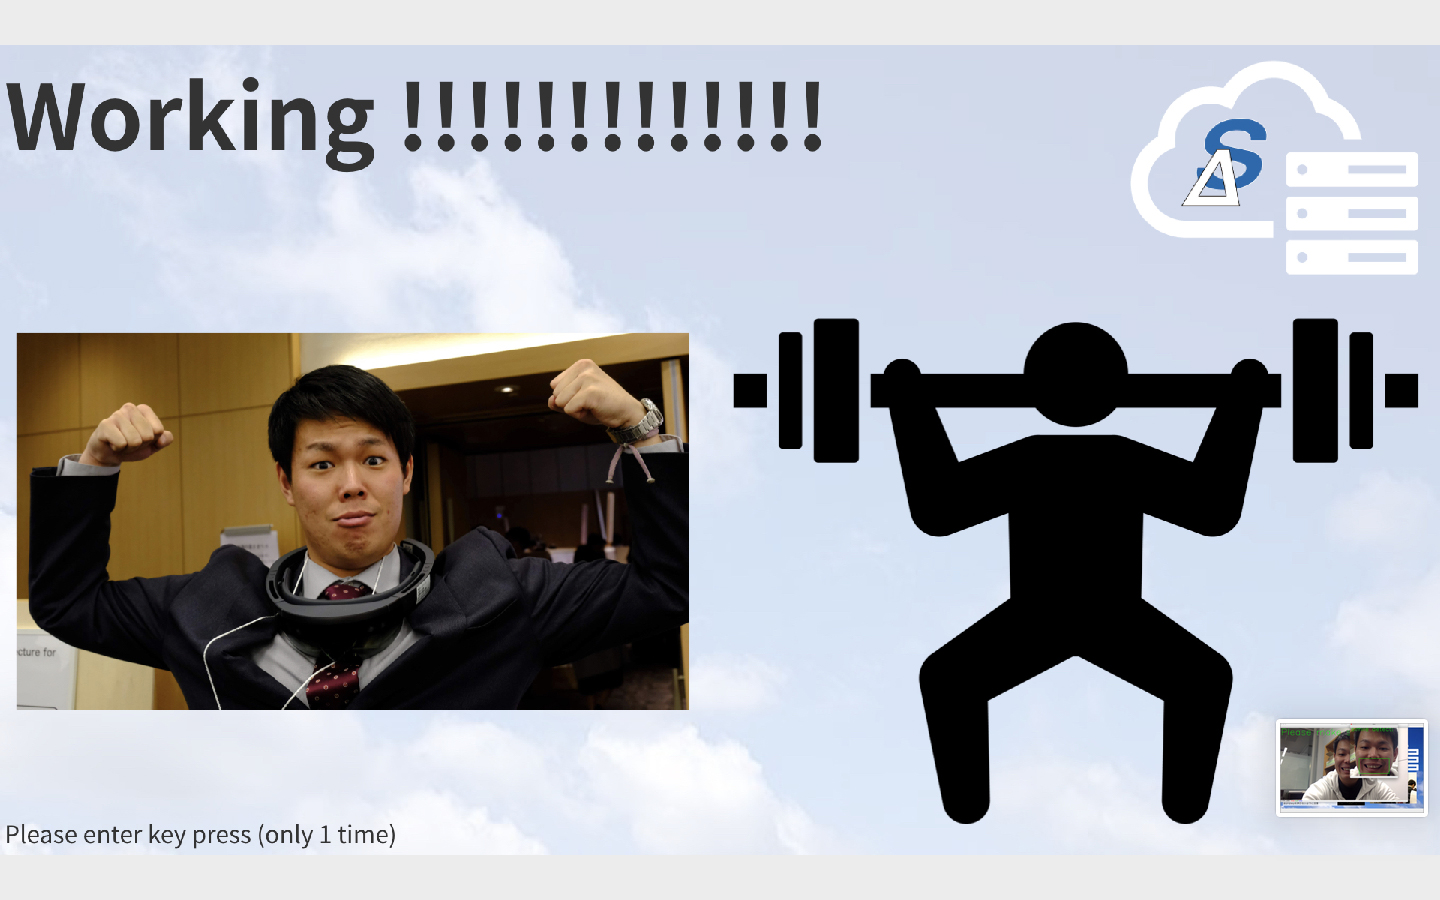
\includegraphics[width=140mm,bb=0 0 1440 900]{seen5.jpg}}
    \end{center}
    \caption{ユーザーインターフェースシーン5}
    \label{fig:seen5}
\end{figure}

\begin{figure}[htbp]
    \begin{center}
       \fbox{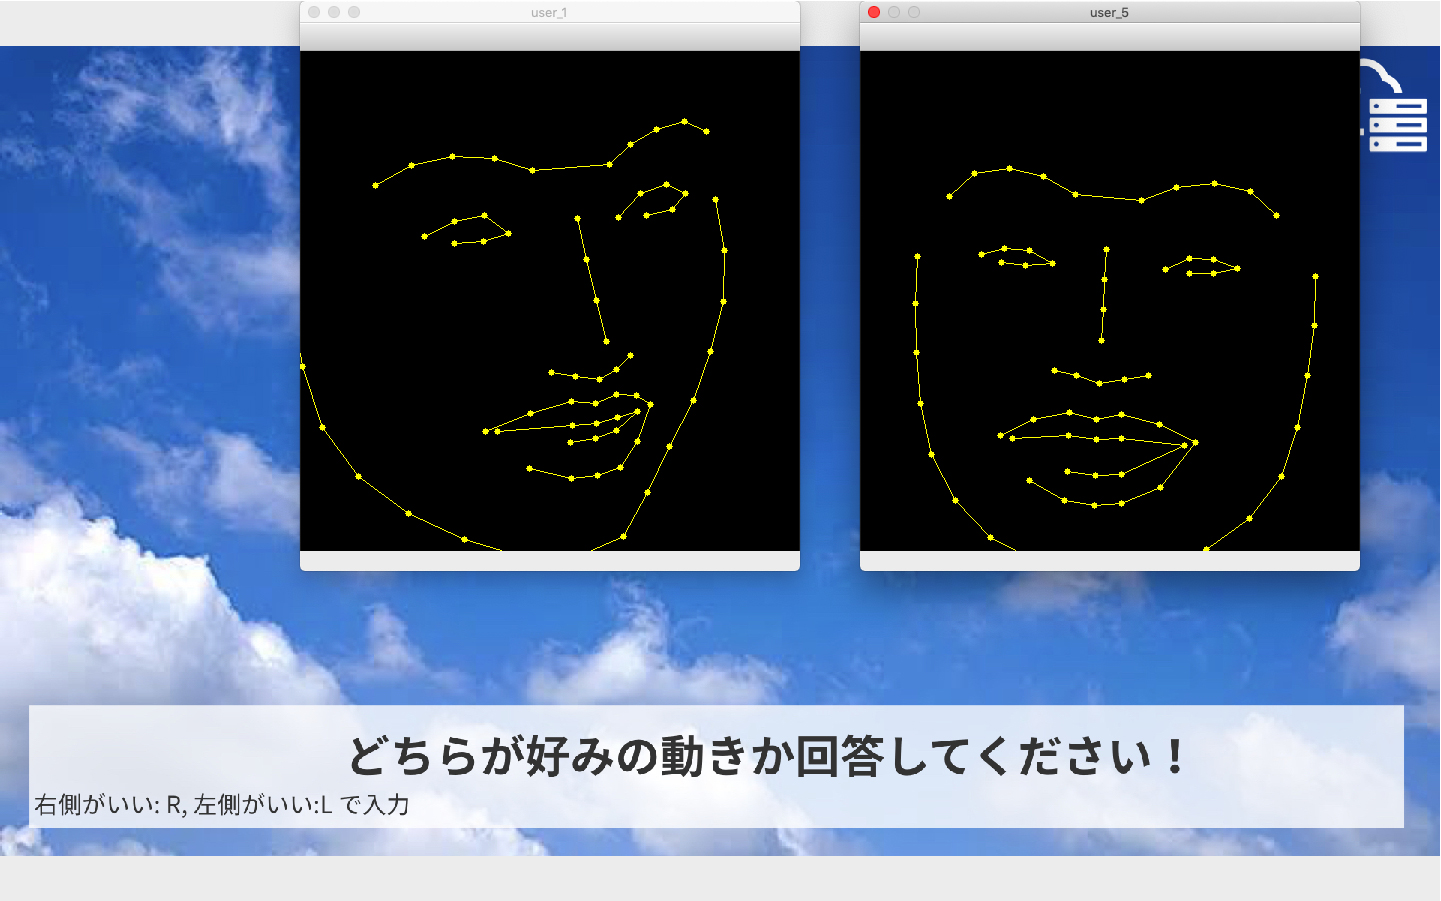
\includegraphics[width=140mm,bb=0 0 1440 900]{seen6.jpg}}
    \end{center}
    \caption{ユーザーインターフェースシーン6}
    \label{fig:seen6}
\end{figure}

\begin{figure}[htbp]
    \begin{center}
       \fbox{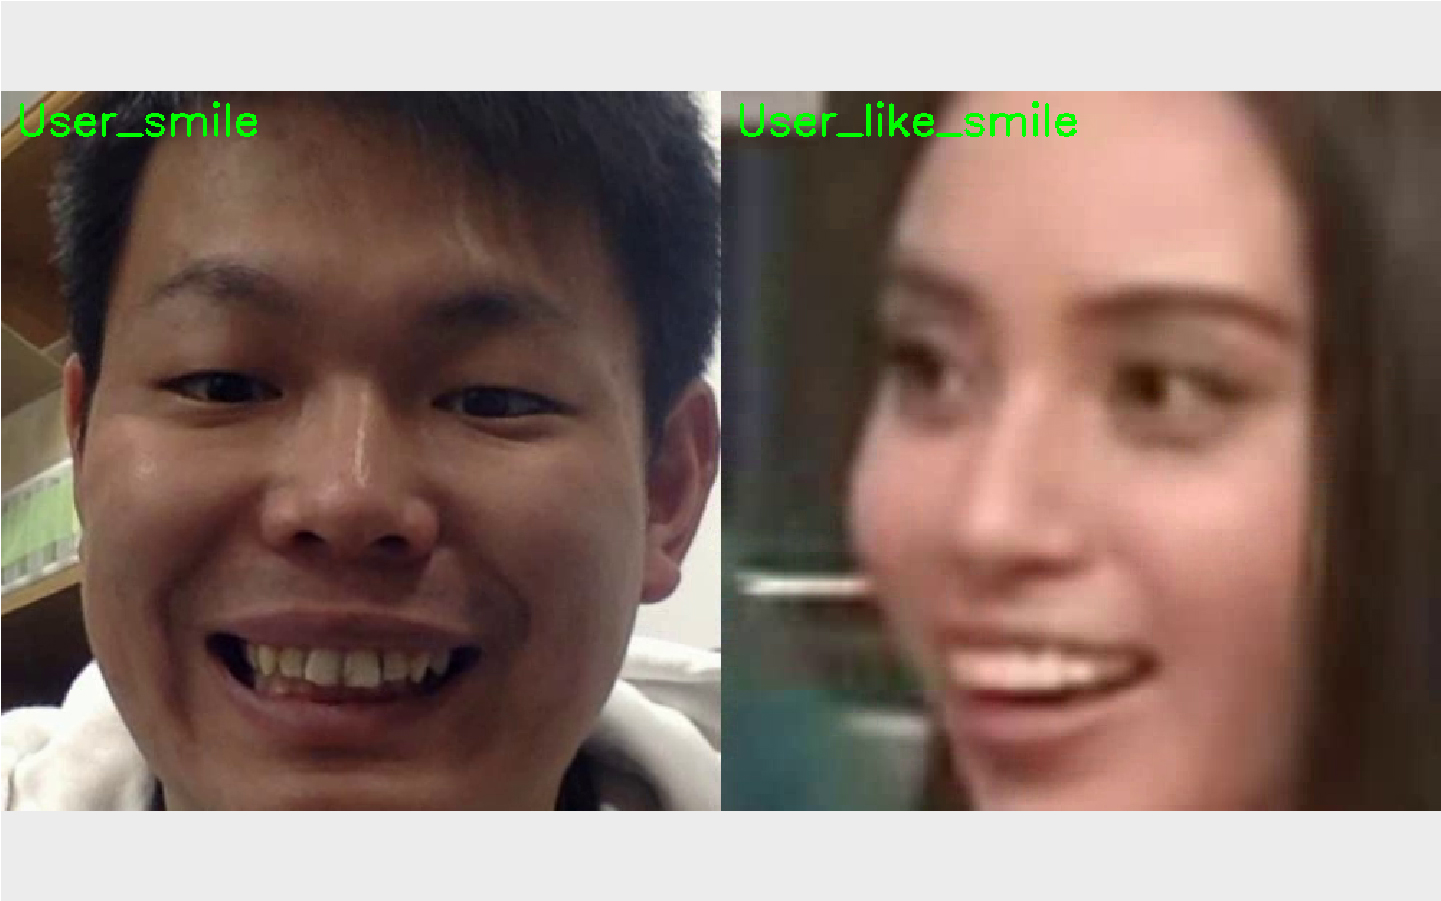
\includegraphics[width=140mm,bb=0 0 1440 900]{seen7.jpg}}
    \end{center}
    \caption{ユーザーインターフェースシーン7}
    \label{fig:seen7}
\end{figure}

\begin{figure}[htbp]
    \begin{center}
       \fbox{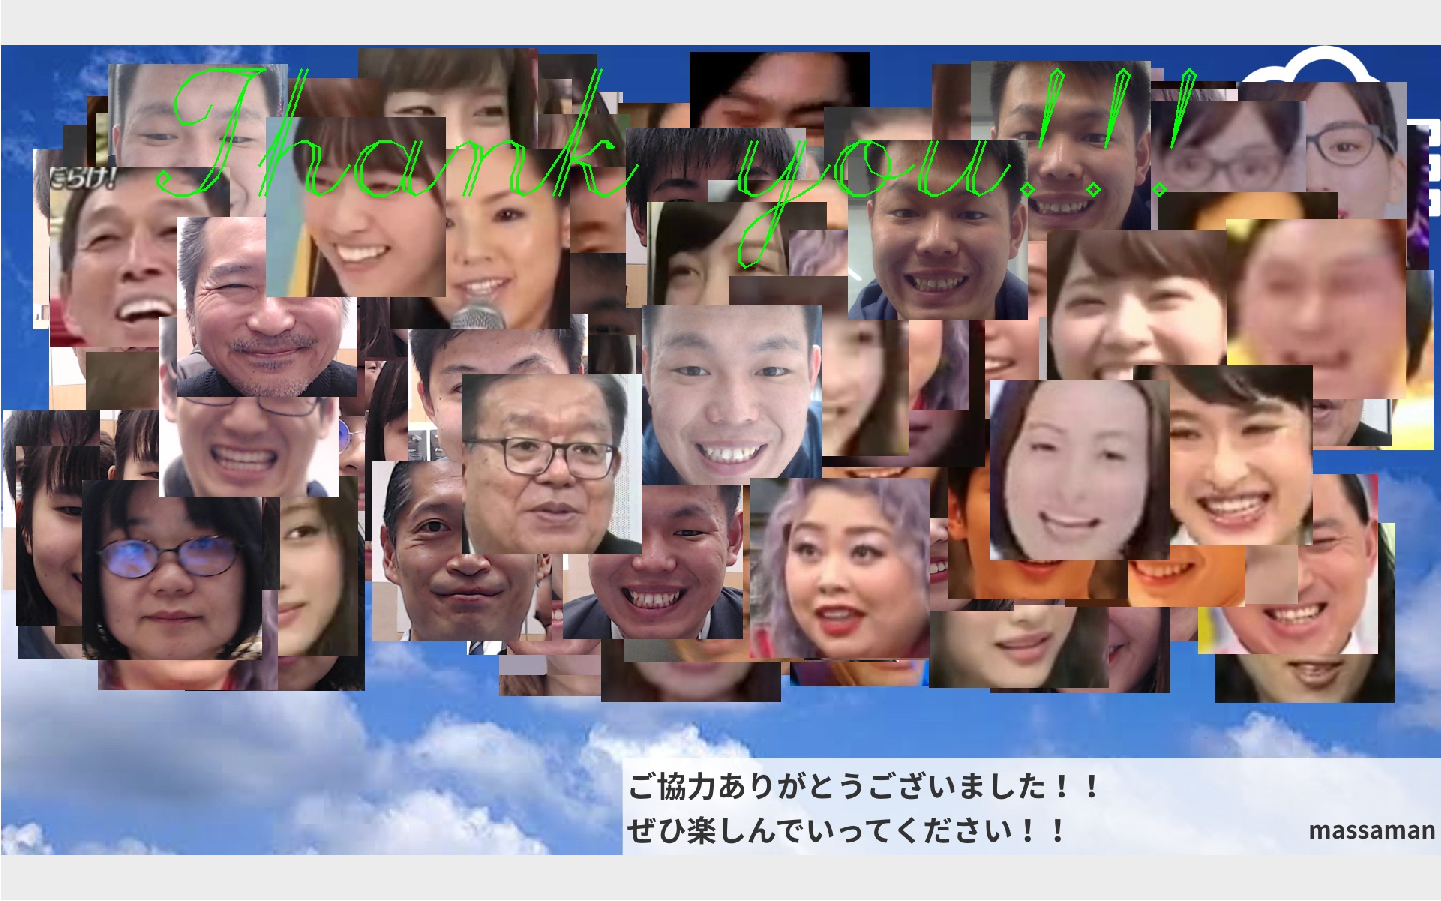
\includegraphics[width=140mm,bb=0 0 1440 900]{seen8.jpg}}
    \end{center}
    \caption{ユーザーインターフェースシーン8}
    \label{fig:seen8}
\end{figure}


\section{データ収集機能の実装}
このセクションでは, 各モジュールの実装の詳細について述べる.

\subsection{顔検出モジュールの実装}
顔検出はオープンソースであるOpenCVの中に含まれるカスケードである,
haarcascade\_frontalface\_default.xmlをOpenCVで読み込み使用する.
読み込んだ全ての動画フレームに対して顔検出の処理を行う.
\begin{itemize}
\item 顔検出検出パラメーター
\begin{lstlisting}
face_list =face_detect_cascade.detectMultiScale(
  gray,scaleFactor = 1.21,
  minNeighbors = 15,
  minSize=(300,300)
  )
\end{lstlisting}
\end{itemize}
検出した全ての動画フレームに対して表示処理を行う場合, システムのラグが発生するため,表示は偶数フレームのみとした.
返り値の画像に含まれる顔の左上のx座標およびy座標, 横幅と高さの値を次の関数へと引き継ぐ.

\subsection{笑顔検出モジュールの実装}
顔検出モジュールで得た返り値の値を参照し,顔のある領域のみに対して笑顔の検出処理を全てのフレームに対して行う.
笑顔の判別はOpenCVの中に含まれるhaarcascade\_smile.xmlを読み込み使用する.
このカスケードは顔の口の領域に対して処理を行い笑顔の検出を行う.
webカメラから取得した画像全ておよび, 全ての領域に対して笑顔検出の処理を行うことも可能であるが,
実装のテスト段階で誤検出が多かったため, 顔を検出しその中でも誤検出が一番少ないパラメータ調整を行った.

\begin{itemize}
\item 笑顔検出パラメーター
\begin{lstlisting}
smile_detector =smile_cascade.detectMultiScale(
  face_gray,scaleFactor= 1.7,
  minNeighbors=20,
  minSize=(120, 120)
  )
\end{lstlisting}
\end{itemize}

顔を検出したフレームが20フレーム以上,および笑顔を検出したフレームが5フレーム以上になった場合に
検出を終了する.

\subsection{画像処理モジュールの実装}
顔検出および笑顔検出モジュールで取得したフレームに対して, 画像処理を行う.
検出したフレームをコンパイルしたOpenFaceのFaceLandmarkImg関数を使用して, 全てのフレームから
顔のパーツの動きを表したFacial Action Unitの値をcsvファイルに算出する.
各フレームごとに生成されるため, ユーザーごとに1つのファイルにマージする処理をここで行う.

\begin{itemize}
\item OpenFace算出パラメータ例:
\begin{lstlisting}
frame, timestamp, confidence, success,
gaze_0_x, gaze_0_y, gaze_0_z, gaze_1_x, gaze_1_y, gaze_1_z,
pose_Tx, pose_Ty, pose_Tz, pose_Rx, pose_Ry, pose_Rz,
x_0, x_1, ... x_67, y_0, y_1, ..., y_67,
X_0, X_1,..., X_67, Y_0, Y_1,..., Y_67, Z_0, Z_1, ... Z_67,
p_scale, p_rx, p_ry, p_rz, p_tx, p_ty, p_0, p_1, ..., p_33,
AU01_r, AU02_r, AU04_r, AU05_r, AU06_r, AU09_r, AU10_r,
AU12_r, AU14_r, AU15_r, AU17_r, AU20_r, AU25_r, AU26_r,
AU04_c, AU12_c, AU15_c, AU23_c, AU28_c, AU45_c
\end{lstlisting}
\end{itemize}

\subsection{動画作成モジュールの実装}
フレームごとに処理をした後, 全てのフレームを時系列順に結合して笑顔動画データの作成を行う.
フレームには保存時にファイル名で時系列順に番号を振っており, 配列にデータを格納しソートすることで
時系列順に処理を行うことが可能である.
本システムにおいて,fps(Frame per Seconds) は20であったため1秒間の動画が生成される.

\subsection{データ作成モジュールの実装}
一番初めに入力したユーザーの基本データ, 画像処理モジュールで生成したCSVファイルおよび動画作成モジュール
で作成したユーザーの笑顔動画データをユーザーごとにファイリングしてデータフォーマットとする.
作成したデータは各ユーザーごと, 各データの種類ごとの2通りの方法でデータを保存する.

\begin{itemize}
\item ユーザーごとのデータツリー構造:
\dirtree{%
 .1 user\_dirname.
 .2 FAU\_data.csv(FAUから取得したデータ).
 .2 FAU\_data\_plot.png(FAUの値を簡易プロットしたグラフ画像).
 .2 user\_info.txt(ユーザーの基本情報).
 .2 rankingdata.csv(ユーザー順位づけデータ).
 .2 output.mp4(ユーザーと選んだ笑顔動画データを並べて表示).
 .2 user\_smile\_video.mp4(ユーザー単体の笑顔動画データ).
}
\end{itemize}

\subsection{笑顔動画データ選択モジュールの実装}
画像処理モジュールで生成したデータの中にあるパラメータp\_scale を使用する.
各フレームのp\_scaleを{\sl pscale\_i}とし, フレームの総数を{\sl n}とすると,
笑顔データ選択の際に使用するユーザーごとの指標user\_pcaleを以下のように定義する.
\begin{equation}
\label{pscalesum}
pscale\_sum = \sum_{i=1}^ n pscale\_i
\end{equation}

\begin{equation}
\label{userpscale}
user\_pscale= \frac{pscale\_sum}{n}
\end{equation}

p\_scaleは第\ref{chap:function}章で示した, 図\ref{fig:face_balance}の様に,
差分λで出力されるため, 各笑顔動画データのλ同士を以下のように比較演算を行う.
ユーザーの指標user\_pcale, データベースの中にある笑顔動画データそれぞれのp\_scaleの値を,
each\_pscaleとし, 差分differenceを以下のように定義する.

\begin{equation}
\label{difference}
difference =
\left(
user\_pcale - each\_pscale
\right)
^2
\end{equation}

数式\ref{difference}を各データごとにもとめ, 配列格納し昇順にソートする.
配列に格納されたデータを$x_i$と表し, 5つのデータを算出し,それぞれのデータのindexを取得する.
以下にデータを選出する際の計算式を記述する.
\begin{equation}
\label{data1}
data_1  = x_1
\end{equation}

\begin{equation}
\label{data2}
data_2 = \left\{ \begin{array}{ll}
\frac{x_{\frac{n}{2}} + x_{\frac{n+1}{2}} }{2} & (データ数が2nの場合,nは自然数) \\
x_{\frac{n}{2}} & (データ数が2n-1の場合,nは自然数)
\end{array} \right.\end{equation}

\begin{equation}
  \label{data3}
  data_3 = \left\{ \begin{array}{ll}
  \frac{x_n + x_{n+1} }{2} & (データ数が2nの場合,nは自然数) \\
  x_n & (データ数が2n-1の場合,nは自然数)
  \end{array} \right.\end{equation}

\begin{equation}
  \label{data4}
  data_4 = \left\{ \begin{array}{ll}
  \frac{x_{\frac{3n}{2}} + x_{\frac{3n+1}{2}} }{2} & (データ数が2nの場合,nは自然数) \\
  x_{\frac{3n}{2}} & (データ数が2n-1の場合,nは自然数)
  \end{array} \right.\end{equation}


\begin{equation}
  \label{data5}
  data_5  = \left\{ \begin{array}{ll}
  x_{2n} & (データ数が2nの場合,nは自然数) \\
  x_{2n-1} & (データ数が2n-1の場合,nは自然数)
  \end{array} \right.\end{equation}

数式\ref{data1}は差分の最小値,つまりユーザーの値をもつ笑顔動画データを示す.
数式\ref{data2}は,第1四分位数,数式\ref{data3}は中央値,
数式\ref{data4}は第3四分位数,数式\ref{data5}は差分の最大値をもつ笑顔動画データをそれぞれ示す.
上記の値によって取得したindexを用いて, 笑顔動画データを5種類選出する.

\subsection{表示データ作成モジュールの実装}
取得した5種類の笑顔動画データを点描画にするための処理を行う.
python のライブラリdlibを使用して顔器官検出を行う.
モデルはshape\_predictor\_68\_face\_landmarks.datを使用し, 顔の特徴点のみを表示する.

\begin{figure}[htbp]
    \begin{center}
       \fbox{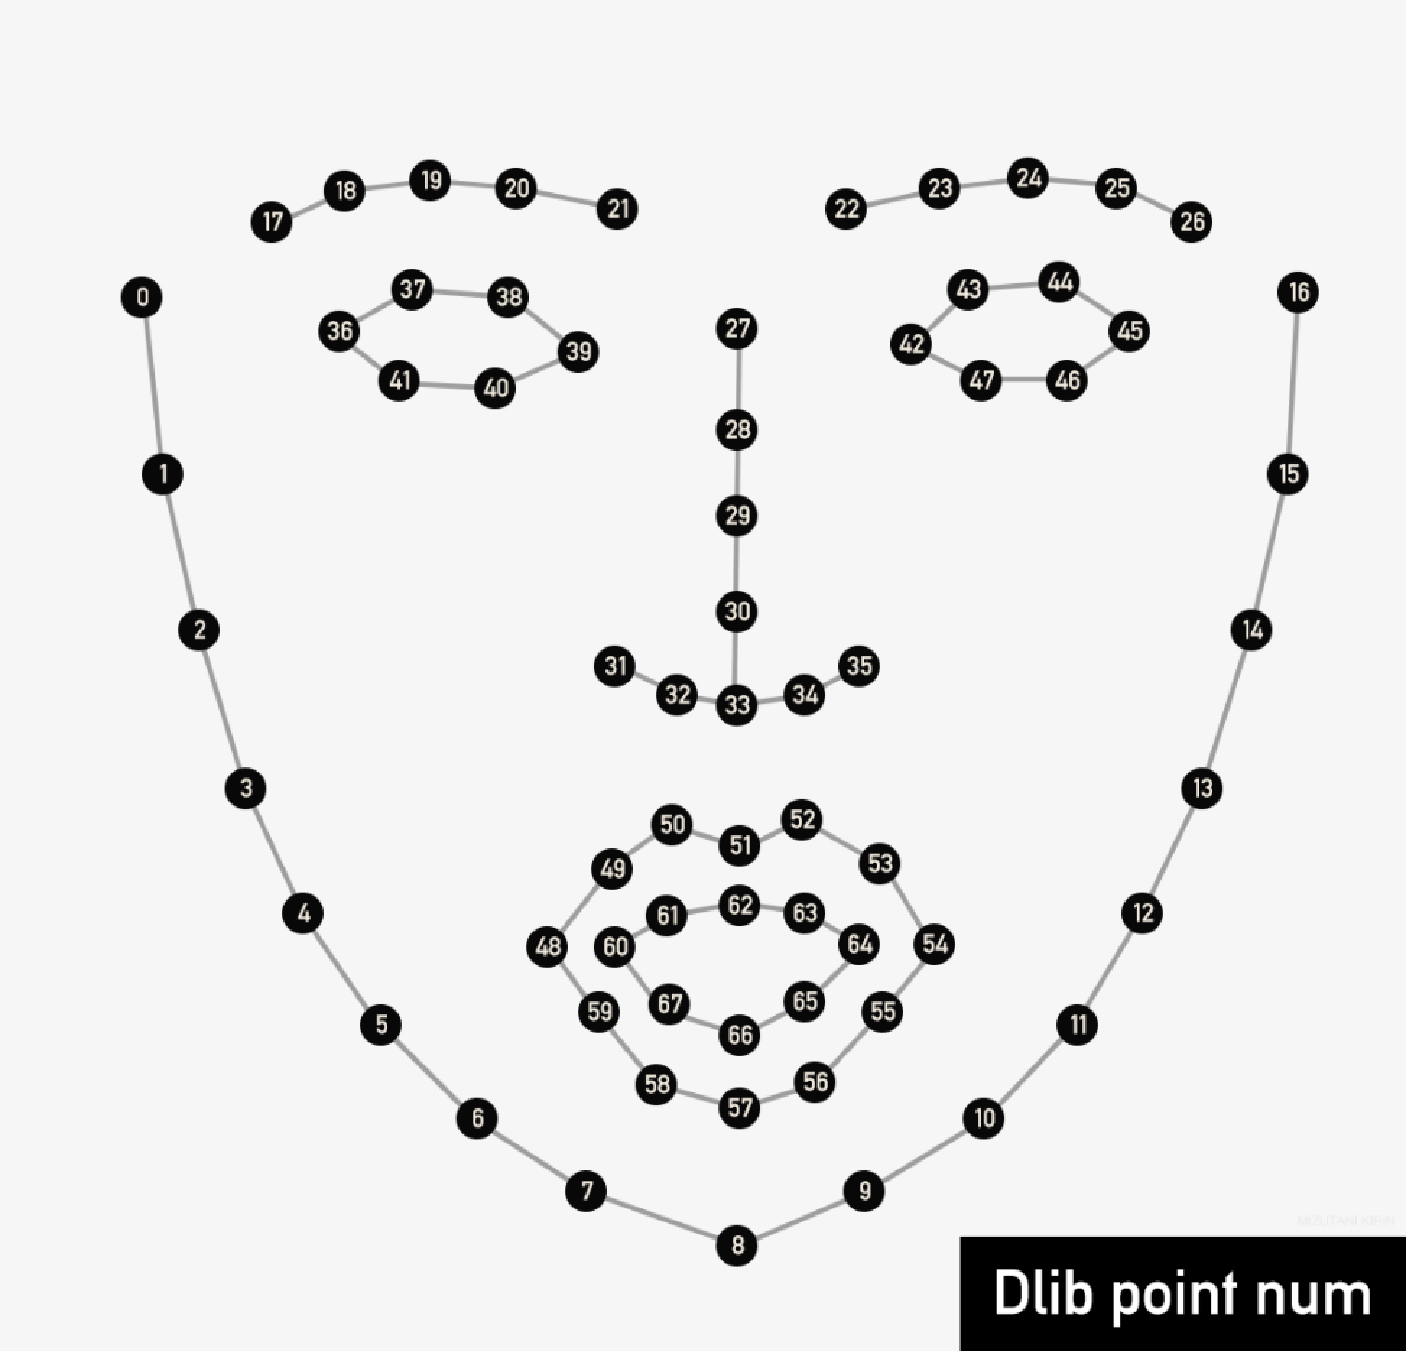
\includegraphics[width=80mm,bb=0 0 1406 1352]{dlibfacepoits.jpg}}
    \end{center}
    \caption{dlibを用いてた特徴点検出}
    \label{fig:dlibfacepoits}
\end{figure}

\begin{figure}[htbp]
    \begin{center}
       \fbox{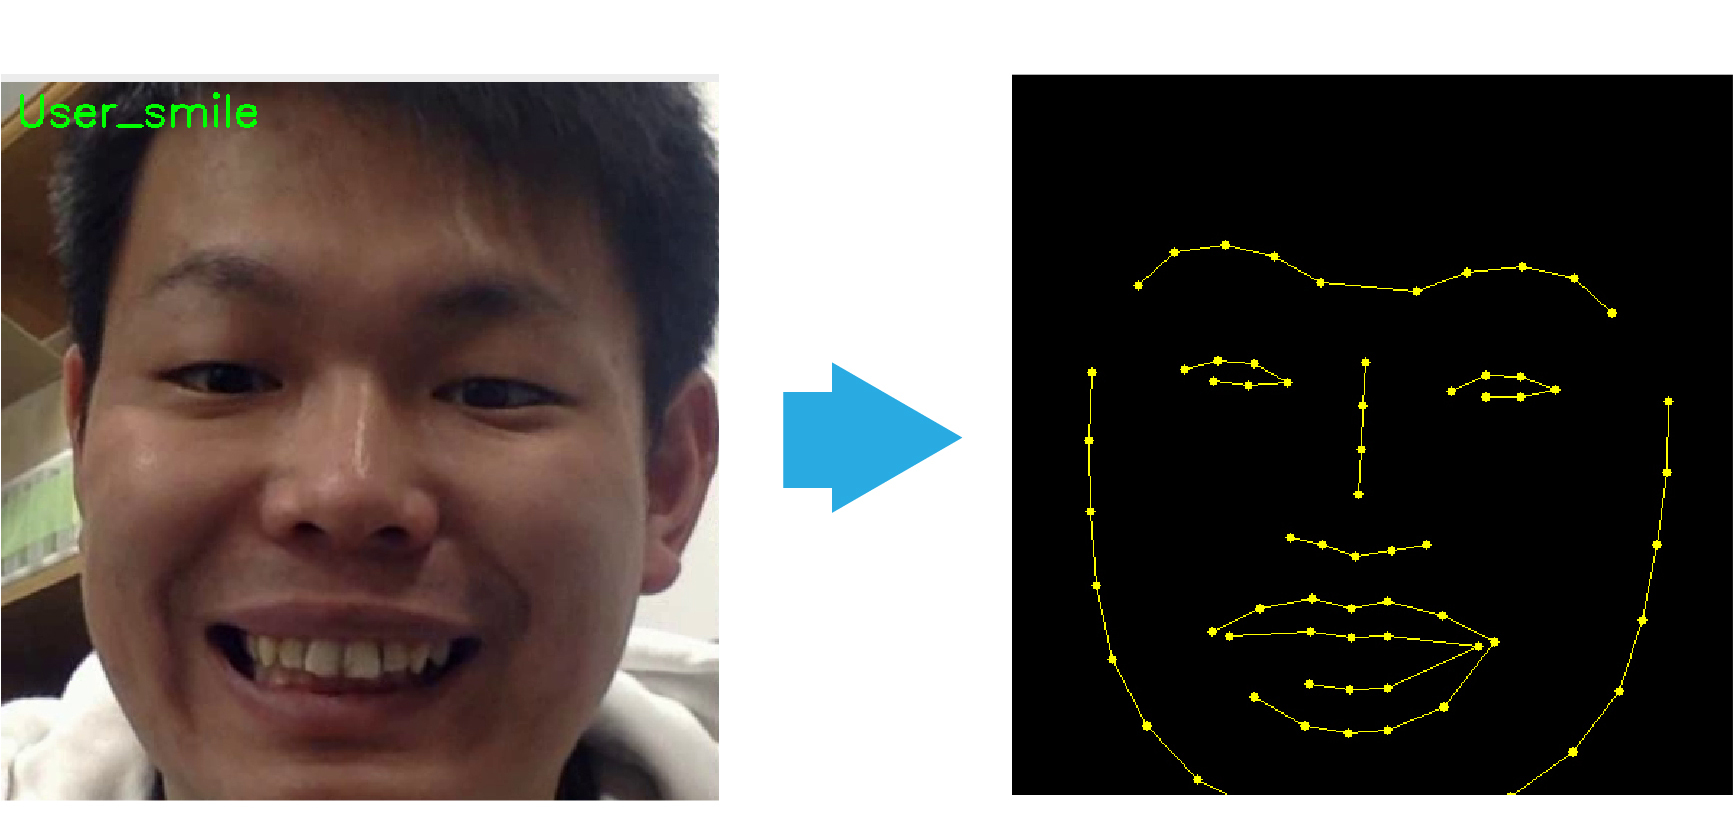
\includegraphics[width=140mm,bb=0 0 1733 827]{face_convert.jpg}}
    \end{center}
    \caption{変換後の動画例}
    \label{fig:face_convert}
\end{figure}

\subsection{順位づけモジュールの実装}
表示データモジュールで作成した動画データを2つずつユーザーに表示し, どちらのほうが好みかを答えてもらい
順位づけを行う. 右側を選んだ場合はR, 左を選んだ場合はLをキーボードから入力し,
選ばれなかった方の動画のpathを記録し, 次の動画を表示する.
4回比較を行い, ユーザーが最後に選んだものから逆順に1番から5番までの順位づけを行い,
それぞれの動画のpathと結びつけた状態で順位づけデータとして記録する.

\subsection{データ保存モジュールの実装}
順位づけデータを取得したのち, データベースから記録された動画pathを使用してユーザーフォルダーに
ユーザー自身のデータを除く4データを保存する. また笑顔動画を解析した結果が記録されているCSVファイルも
同時に保存し, 分析に使うデータの整理を行う.

\begin{itemize}
\item データ整理後のユーザーごとのツリー構造:
\dirtree{%
 .1 user\_dirname.
 .2 FAU\_data.csv(FAUから取得したデータ).
 .2 FAU\_data\_plot.png(FAUの値を簡易プロットしたグラフ画像).
 .2 user\_info.txt(ユーザーの基本情報).
 .2 rankingdata.csv(ユーザー順位づけデータ).
 .2 output.mp4(ユーザーと選んだ笑顔動画データを並べて表示).
 .2 user\_smile\_video.mp4(ユーザー単体の笑顔動画データ).
 .2 userFAUcsv.
 .3 AU06\_c.csv.
 .3 AU06\_r.csv.
 .3 AU07\_c.csv.
 .3 AU07\_r.csv.
 .3 AU12\_c.csv.
 .3 AU12\_r.csv.
 .3 AU25\_c.csv.
 .3 AU25\_r.csv.
 .3 merge.csv.
 .2 csvdir.
 .3 no1.csv.
 .3 no2.csv.
 .3 no3.csv.
 .3 no4.csv.
 .3 no5.csv.
 .2 videodir.
 .3 no1.mp4.
 .3 no2.mp4.
 .3 no3.mp4.
 .3 no4.mp4.
 .3 no5.mp4.
}
\end{itemize}

\subsection{選択データ表示モジュールの実装}
最後にユーザーの順位づけデータを基に, 順位づけが一番高かった笑顔動画データをユーザーの笑顔動画データ
と並べて表示する. output.mp4の動画形式で保存しユーザーが点描画で選んだ笑顔動画データの基になっている
オリジナルの動画データを表示することで, ユーザーへのフィードバックを行う.
また, 現時点では個人が特定できるような名前や年齢などパーソナルな情報は公開せずに, 笑顔動画データのみを
相手に表示する形を取っている.

\section{データ分析機能の実装}
作成中...
\subsection{FAU値計算モジュールの実装}
\subsection{データプロットモジュールの実装}
\section{まとめ}
本章では, 本システムにおけるユーザーインターフェースの実装および, データ収集機能の各モジュールの実装,
データ分析機能の各モジュールの実装についてまとめた.
次章では本研究における予備実験について述べる.
  % 実装
\chapter{予備実験}
\label{chap:pre_experiment}

この章では本研究で行った予備実験について述べる.
本予備実験の目的は, 本実験の際に本システムの処理が妥当であることを証明するためのものとした.
まず笑顔データを作成する際のフレーム数および秒数の指定についてシステムの予備実験を行い,
次に笑顔の動画データを収集する際に使用する採用モデルの評価を行なった.
\section{表情を作るのかかる時間}
本システムはユーザーの顔を認識し, その表情の変化を記録し表情分析を行う.
ユーザーへ笑顔動画データをフィードバックをする際には, 人間が表情の変化を認識することができるフレーム数を
確保しなければならない.
織田らの瞬間的に変化する表情を人がどの程度正確に認知をすることができるのかを検証した研究では,
笑顔と怒りの場合は, 200m\/s まで高い認知をすることが可能であると述べている.\cite{織田朝美2005表情の瞬間的変化の認知}

\subsection{実験}
本システムを起動し, 自身のラップトップPCがどれだけのフレームレート(fps)でユーザーの記録を行うことができるのかを検証する.
取得したfpsの値を用いて, 織田らが明示した1フレーム辺りの表示時間が200ms  以上,
つまりミリフレームレート(fpms)が200以下であることを確認する.

\subsection{結果}
\begin{itemize}
\item 実行結果
\setlength{\parskip}{20pt}
\begin{lstlisting}
start_from_webcam
FPSの設定値、video.get(cv2.CAP_PROP_FPS) : 20.0
\end{lstlisting}
%複数の時は以下のように
%\item 実行コマンド
%\begin{lstlisting}
%$ python dsfsa.py mode_num
%\end{lstlisting}
\end{itemize}
本システムにおけるfpsは20であったため, 1秒間に20フレームを取得することができている.
よって,これをミリフレームレート(fpms)に変換すると,
\begin{equation}
\label{fpms}
 fpms = \frac{1000.0}{20.0} = 50.0
\end{equation}
となる.
よって, 人が認知に必要な200ms以上フレームを取得し, 表示することができているためこのシステムは
人の表情の変化を知覚する条件を満たしていることが証明できた.


\section{OpenCVを使った笑顔検出の妥当性}
本システムでは収集した笑顔動画データを解析する際には, Cambridge大学が開発したオープンソースの
OpenFace を使用している. 顔パーツの位置や, Facial Action Units (以下FAU)によって表情を
判断するパーツの動きの強度を取得することが可能である.
しかし, 開発途中のオープンソースおよび有用なデータを1フレームに対して, 711個データを取得するため
処理時間が長くなってしまう.

pythonの中に含まれる, cProfileを使用して静止画,
1フレームの時間を取得すると, 平均約4secの処理時間がかかることが判明し, さらに本研究で採用している20フレーム分の処理を行なった場合,
20秒の処理時間を要することが判明した.
以上のことより, 笑顔動画データを作成するためのフレーム取得にはより処理速度の速いOpenCVの中に含まれる
haarcascades\/ haarcascade\_ smile.xmlの笑顔判定モデルを使用した.

 \begin{itemize}
   \setlength{\parskip}{20pt}      %4. 段落間余白
 \item 処理時間時間計測
 \begin{lstlisting}
 $ python -m cProfile -s tottime dsfsa.py
 \end{lstlisting}
 \end{itemize}

\subsection{実験}
OpenCvの笑顔判定モデルを使用して, 人が映っている動画データに対して笑顔検出を行う.
笑顔のフレームを一番最後に5フレーム含み, 全体20秒の笑顔動画データを作成する.
作成した笑顔動画データに対してOpenFaceの処理を行い, 最後のフレームに対して笑顔のFAUである
FAU06(眼窩部眼輪筋)とFAU12(大頬骨筋)の判定値が検出できるかどうかを判定する.
実験はテストデータ3つに対して行った.

\subsection{結果}
OpenCVの笑顔認識モデルを使用して作成した笑顔動画データに対して, OpenFaceの処理を行なった結果を
図\ref{fig:preex1},\ref{fig:preex2},\ref{fig:preex3} に出力した.
各データともに, FAU06およびFAU12(大頬骨筋)の値を検出することができた.
よってデータ収集の際に, OpenCVの笑顔判別器を使用してデータ収集をすることは可能であることがわかった.

\begin{figure}[htbp]
  \setlength\intextsep{0pt}
    \begin{center}
       \fbox{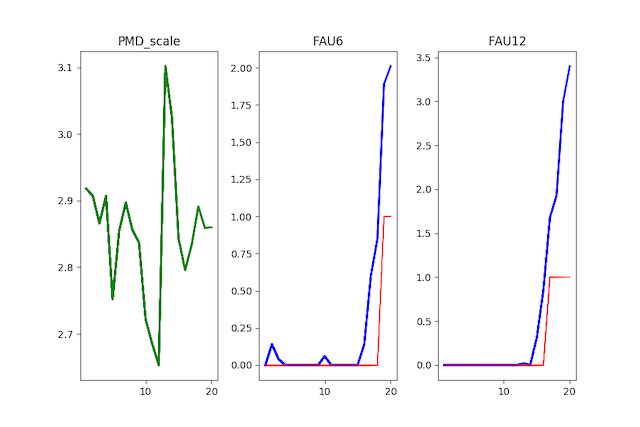
\includegraphics[width=150mm,bb=0 0 600 427]{preex1.jpg}}
    \end{center}
    \caption{笑顔動画データ1}
    \label{fig:preex1}
\end{figure}

\begin{figure}[htbp]
  \setlength\intextsep{0pt}
    \begin{center}
       \fbox{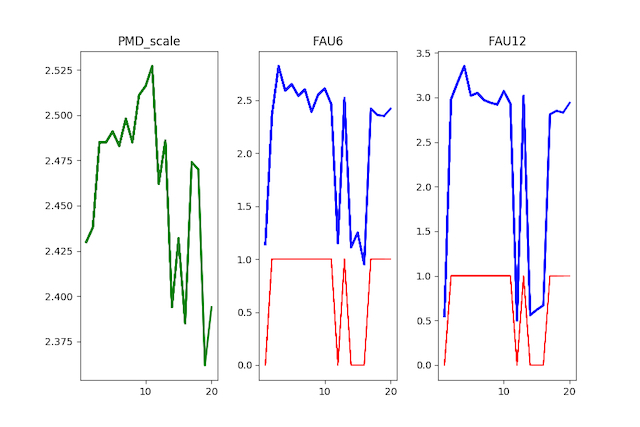
\includegraphics[width=150mm,bb=0 0 640 427]{preex2.jpg}}
    \end{center}
    \caption{笑顔動画データ2}
    \label{fig:preex2}
\end{figure}
\begin{figure}[htbp]
  \setlength\intextsep{0pt}
    \begin{center}
       \fbox{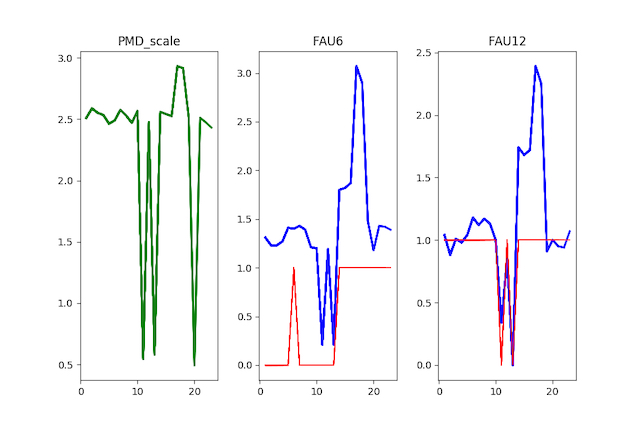
\includegraphics[width=150mm,bb=0 0 640 427]{preex3.jpg}}
    \end{center}
    \caption{笑顔動画データ3}
    \label{fig:preex3}
\end{figure}

\section{実験の結果・まとめ}
本章では, 本システムが実験をする際の条件を満たしているかの予備実験を行なった.
次章では本システムを用いた評価実験について述べる.
  % 予備実験
\chapter{評価実験}
\label{chap:main_experiment}

この章では本研究で行った評価実験について述べる.

\section{評価実験の概要}
\section{評価実験の目的}
\section{ORF(Open Research Forum)におけるデータ収集}
\section{ユーザーの嗜好分析}

\section{地震の表情の作り方と好感をもつ笑顔との相関性}
\section{結果}
\section{まとめ}
  % 本実験
\chapter{結論}
\label{chap:conclusion}

この章では本研究における結論について述べる.
まず今後の展望について述べ, 次に具体的なデータの収集・活用方法について述べる,
最後に本研究のまとめを行い,卒業論文とする.

\section{今後の展望}
第\ref{chap:main_experiment}章の評価実験において, 人は一度顔の筋肉を弛緩してから笑顔になるユーザーに対して嗜好傾向がある可能性を示した.
しかし, 本研究では被験者41人, 有効データ36個と非常に傾向分析には少ないデータとなってしまっている.
さらに, データの大半は20代および男性のデータが約68\%と偏りのあるデータとなってしまっている.
今後, 追加データを取得する際には設置場所を考慮し,バランスのとれたデータを取得する必要がある.
また, 本研究は表情ベースでの判断のみになってしまっており, ここの内面状態やどのような基準で
順位づけを行っているのかを考慮することができていない.
Open Research Forum においてユーザー1人,1人へインタビュー調査を行うことは叶わなかったため,
今後は表情ベースの判断に加え, 内面的状態を考慮してデータを提案することが可能なシステム
構成を考える必要がある.

\subsection{TEAM Smileとの連携}
私は慶應義塾大学湘南藤沢キャンパス中澤仁研究室が関与している健康情報コンソーシアムの中にある
Team SMILEに参加し, SmileMeterの開発に携わっている.\cite{teamSMILE}SmileMeterとは自分の笑顔状態を把握し,
自分で安全に保存・蓄積できる、素敵なキオスクデバイスである.
今までに玉川高島屋や, イオンモール幕張新都心, 地域のイベントなどに出展をし,
笑顔と健康の大切さを伝える活動を行っている.
今後,TeamSmileの活動が発展していく上でより多く, 精度の高いデータを集取し活動に活かすために
本システムで作成したOpenFaceを使用した表情解析モジュールをSmileMeterに組み込む予定である.
実証実験の場が今後増えていき, より多くのデータを取得することが見込まれる.
本研究では40人といった小規模実験を行ったが,  より多く幅広い年齢・性別のデータを分析することで
より人と人とを繋ぐシステムを構築するためのデータを取得する.

\begin{figure}[htbp]
    \begin{center}
       \fbox{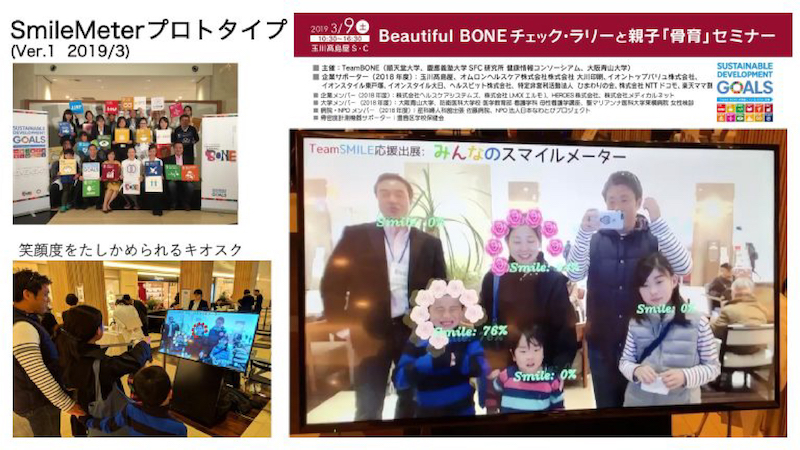
\includegraphics[width=150mm,bb=0 0 800 450]{takashimaya.jpg}}
    \end{center}
    \caption{玉川高島屋の出展}
    \label{fig:takashimaya}
\end{figure}

\begin{figure}[htbp]
    \begin{center}
       \fbox{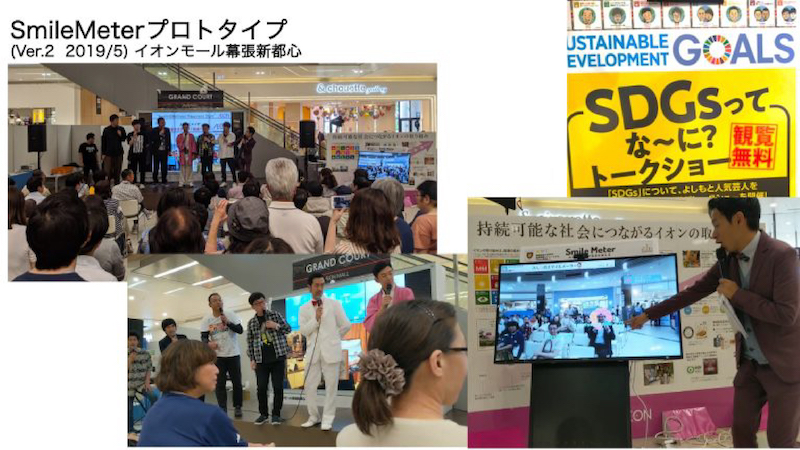
\includegraphics[width=150mm,bb=0 0 800 450]{aeon.jpg}}
    \end{center}
    \caption{イオンモール幕張新都心の出展}
    \label{fig:aeon}
\end{figure}

\begin{figure}[htbp]
    \begin{center}
       \fbox{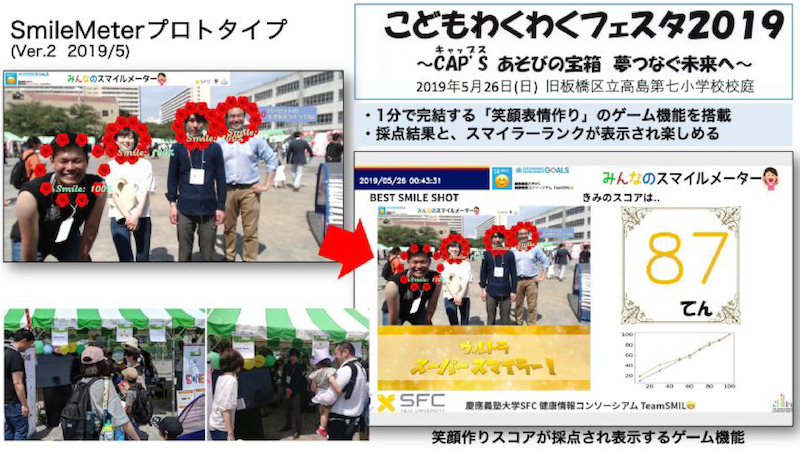
\includegraphics[width=150mm,bb=0 0 800 450]{itabashi.jpg}}
    \end{center}
    \caption{板橋区イベントの出展}
    \label{fig:itabashi}
\end{figure}

\subsection{1月下旬に行った実証実験について}
TeamSMILEの共同研究をしている福岡の株式会社LMOの九州良縁フェスティバルに2020年1月18日鹿児島,
19日熊本に参加した. 本イベントは, 20代以上の独身男女が参加する結婚活動イベントであり,
TeamSMILEはSmileMeterを展示し,来場者にむけて実証実験を行った.
将来のパートナーを決める際には, 自分の運命を大きく作用するため相手選びがより慎重になる.
重要な選択をする際に, 自身や相手の根本的な部分を表情によって分析し, 情報提供をすることができれば
より自分にも相手にとっても良好な人間関係の構築をすることが可能になる.
実際に, SmileMeterを体験したカップルには笑顔が増えシステムがお互いにコミュニケーションの
きっかけとなるような働きをしているように思われた.
今後, 本システムの表情解析モジュールを導入し, 良縁な関係を築いていくきっかけになる,
そしてユーザーごとの引き合わせをすることができるシステムの構築を将来的な展望とする.

\begin{figure}[htbp]
    \begin{center}
       \fbox{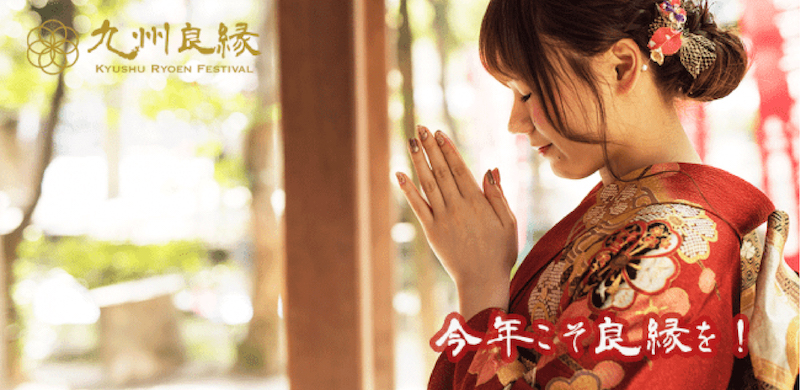
\includegraphics[width=150mm,bb=0 0 800 390]{lmo.jpg}}
    \end{center}
    \caption{株式会社LMOとの共同イベント}
    \label{fig:lmo}
\end{figure}

\begin{figure}[htbp]
    \begin{center}
       \fbox{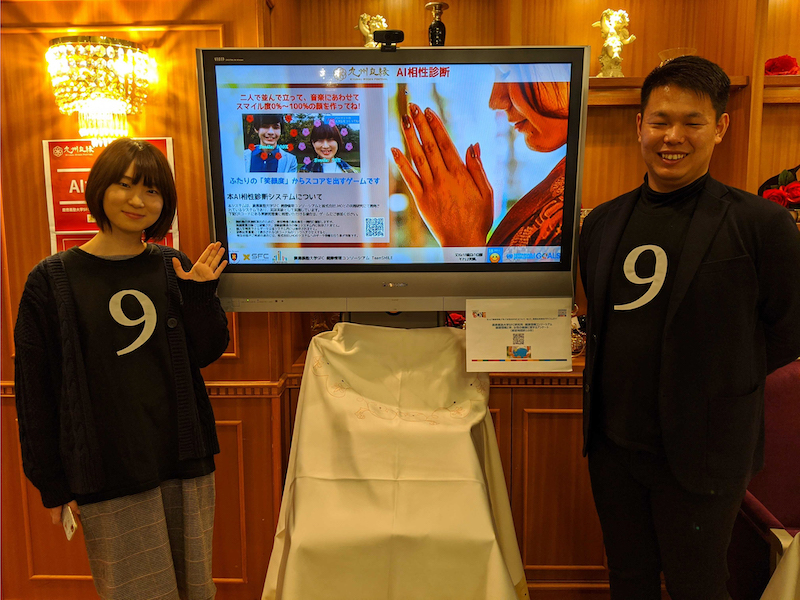
\includegraphics[width=150mm,bb=0 0 800 600]{kyushu.jpg}}
    \end{center}
    \caption{株式会社LMOとの共同イベント当日}
    \label{fig:kyushu}
\end{figure}

\section{本論文まとめ}
本研究は自身の笑顔の作り方と表情ベースによる嗜好判断分析を行った.
41人に対して, 36個の有効笑顔動画データおよびFAU値を取得することができた.
取得したデータの分析により, 人は一度表情の筋肉を弛緩してから笑顔になる笑い方に惹かれている
傾向がみられた.
今後, TeamSmileの活動等を通じて多くのデータを取得し, 本研究, 本システムが人と人とを繋ぐ役割を担うようなシステムになることを期待して卒業論文とする.
  % まとめ


\begin{acknowledgment}
謝辞!!!\\
感謝の言葉を述べる方々はたくさんいらっしゃる...\\
アブストラクトを書いて, 本当の締めで書く.\\
RGの先生方, 仁さん, 大越さん, 陳さん, 柘植さん, 友隆さんを始めとする中澤研究室のファカルティーの方々\\
kgの垣根を超えた大学院の先輩方\\
wataruさん, isokichiさん, drgnmanさん, iphooさんの博士の先輩方,\\
eigenさん,quantan,mokkyさん, ozaさんの修士の先輩方.\\
そしてなにより親のshinsan.\\
兄妹のyuniを始めとする,kg-HAISYSの同期・後輩たち, 中澤研究室の同期後輩たち\\
野中先生のお名前もいれたい, 野中研の研究室メンバーも.\\
そして両親に挨拶をして論文を終わる予定\\

\end{acknowledgment}
  % 謝辞。要独自コマンド、include先参照のこと

\begin{bib}[100]
% BibTeXを使う場合
\bibliography{main}

%\begin{thebibliography}{#1}
%
%  \bibitem{参照用名称}
%    著者名: 
%    \newblock 文献名,
%    \newblock 書誌情報,出版年.
%
% \bibitem{hoge09}
%   ほげ山太郎,ほげ山次郎:
%   \newblock ほげほげ理論のHCI分野への応用,
%   \newblock ほげほげ学会論文誌,Vol.31,No.3,pp.194-201,2009.
% 
% \bibitem{hoge08}
%   Taro Hogeyama, Jiro Hogeyama:
%   \newblock The Theory of Hoge,
%   \newblock {\it The Proceedings of The Hoge Society}, 2008.
%	
%\end{thebibliography}

\end{bib}
  % 参考文献。要独自コマンド、include先参照のこと
\appendix
\chapter{付録の例}

付録を無理矢理出力させるため、てきとうなことを書く。

\section{ほげ}

コマンドは本文と一緒。

\subsection{ふー}

本文と一緒。

\section{ほげほげ}

本文と一緒。

\subsection{ふーふー}

本文と一緒。
    % 付録

\end{document}
